\documentclass[a4paper,12pt,twoside]{book}

\sloppy
% \frenchspacing
\setlength{\unitlength}{1cm}

\usepackage{verbatim}
\usepackage{cite}
\usepackage[dvips]{color}
\usepackage{graphicx}
\usepackage{amsmath}
\usepackage{amssymb}
\usepackage{amsfonts}
\usepackage{mathrsfs}
\usepackage{a4wide}
\usepackage{fancyheadings}
\usepackage[footnotesize,bf]{caption}
\usepackage{makeidx}
%Preparations for multiple indices
\usepackage{multind}

%%%%%%%%%%%%%%%%%%%%%%%%%%%%%%%%%%%%%%%%
\usepackage{ae,aecompl} % only for Type 1 fonts for readable pdf convert

\newcommand{\capdef}{}
\newcommand{\mycaption}[2][\capdef]{\renewcommand{\capdef}{#2}%
        \caption[#1]{{ %\itshape
 {\footnotesize #2}}}}
\makeatletter
\renewcommand{\fnum@table}{\textbf{\tablename~\thetable}}
\renewcommand{\fnum@figure}{\textbf{\figurename~\thefigure}}
\makeatother

% Index: use "makeindex Manual" to create .ind file
%\makeindex

\makeindex{norm}
\makeindex{constants}
\makeindex{api}
\makeindex{aedl}

\newcommand{\bi}{\begin{itemize}}
\newcommand{\ei}{\end{itemize}}
\newcommand{\ra}{$\rightarrow$}
\newcommand{\be}{\begin{equation}}
\newcommand{\ee}{\end{equation}}
\newcommand{\bea}{\begin{eqnarray}}
\newcommand{\eea}{\end{eqnarray}}
\newcommand{\nn}{\nonumber}
\newcommand{\ldm}{\Delta m_{31}^2}
\newcommand{\sdm}{\Delta m_{21}^2}
\newcommand{\deltacp}{\delta_{\mathrm{CP}}}
\newcommand{\stheta}{\sin^2 2 \theta_{13}}

\newcommand{\ie}{{\it i.e.}}
\newcommand{\Ie}{{\it I.e.}}
\newcommand{\eg}{{\it e.g.}}
\newcommand{\Eg}{{\it E.g.}}
\newcommand{\cf}{{\it cf.}}
\newcommand{\etc}{{\it etc.}}
\newcommand{\eq}{Eq.}
\newcommand{\eqs}{Eqs.}
\newcommand{\Def}{Definition}
\newcommand{\fig}{Fig.}
\newcommand{\Fig}{Fig.}
\newcommand{\figs}{Figs.}
\newcommand{\Figs}{Figs.}
\newcommand{\Ref}{Ref.}
\newcommand{\Refs}{Refs.}
\newcommand{\Sec}{Sec.}
\newcommand{\Secs}{Secs.}
\newcommand{\Chapt}{Chapter}
\newcommand{\Chapts}{Chapters}
\newcommand{\Part}{Part}
\newcommand{\App}{Appendix}
\newcommand{\Apps}{Appendices}
\newcommand{\Tab}{Table}
\newcommand{\Tabs}{Tables}

\newcommand{\JHFSK}{{\sc JHF-SK}}
\newcommand{\NUMI }{{\sc NuMI}}
\newcommand{\ReactorI}{{\sc Reactor-I}}
\newcommand{\ReactorII}{{\sc Reactor-II}}
\newcommand{\JHFHK}{{\sc JHF-HK}}
\newcommand{\NuFactI}{{\sc NuFact-I}}
\newcommand{\NuFactII}{{\sc NuFact-II}}
\newcommand{\SPL}{{\sc SPL}}
\newcommand{\Beta}{{\sc $\beta$-Beam}}

\newcommand{\GLOBES}{{\sf GLoBES}}
\newcommand{\AEDL}{{\sf AEDL}}
\newcommand{\EDM}{{\sf EDM}}

\newcommand{\equ}[1]{\eq~(\ref{equ:#1})}
\newcommand{\figu}[1]{\fig~\ref{fig:#1}}
\newcommand{\tabl}[1]{\Tab~\ref{tab:#1}}
\newcommand{\tb}{\hspace*{3ex}}

% Set as GLoBES command and add to index:
% Always use GLB when mentioning a command in text!
\newcommand{\GLB}[1]{{\tt glb#1}\index{api}{#1@{\tt #1}}}
% Always use GLBNS when adding a command to the index without showing it!
\newcommand{\GLBNS}[1]{\index{api}{#1@{\tt \protect{#1}}}}

% Set as GLoBES command and add to index:
% Always use GLB when mentioning a command in text!
\newcommand{\GLBC}[1]{{\tt #1}\index{constants}{\protect{\tt{#1}}}}
% Always use GLBNS when adding a command to the index without showing it!
\newcommand{\GLBNSC}[1]{\index{constants}{{\protect{\tt #1}}}}
\newcommand{\gq}[1]{\begin{quote} {\tt #1} \end{quote}}
\newcommand{\go}[1]{$\rightarrow$ Output: \begin{quote} {\sf #1} \end{quote}}

\definecolor{light}{gray}{0.93}
\definecolor{heavy}{gray}{0.35}
\setlength{\fboxrule}{0.1cm}
\newcommand{\example}[2]{
\begin{table}[p]
\begin{center}
\fcolorbox{heavy}{light}{
\begin{minipage}[t][\textheight][t]{15.5cm}
{\em \underline{Example:} #1}

\vspace*{0.3cm}

#2

\end{minipage}
}
\end{center}
\end{table}
}


\newtheorem{function}{Function}[chapter]

%-- page parameters -------------------------------------------------

\pagestyle{fancyplain}

% Olddefs:

%\addtolength{\textwidth}{-1truecm}
%\addtolength{\oddsidemargin}{1.0truecm}
%\addtolength{\evensidemargin}{-0.3truecm}

% Owndefs:

%\addtolength{\textwidth}{0.0truecm}
%\addtolength{\textheight}{1.8truecm}
%\addtolength{\topmargin}{-0.6truecm}
%\addtolength{\oddsidemargin}{0.65truecm}
%\addtolength{\evensidemargin}{-1.0truecm}

% Headdefs:

\advance \headheight by 3.0truept       % for 12pt mandatory...
\lhead[\fancyplain{}{\thepage}]{\fancyplain{}{\rightmark}}
\rhead[\fancyplain{}{\leftmark}]{\fancyplain{\thepage}{\thepage}}
\cfoot{}

\renewcommand{\chaptermark}[1]{
% chapter title im Seitenkopf
\markboth{\uppercase{\chaptername}\ \thechapter.\ \ #1}
          {\uppercase{\chaptername}\ \thechapter.\ \ #1}}
% section title im Seitenkopf
\renewcommand{\sectionmark}[1]{\markright{\thesection\ \ #1}}




\begin{document} 

\pagenumbering{Roman}
\thispagestyle{empty}
{
\setlength{\parindent}{0cm}

%\begin{titlepage}

\font\fa=cmssbx14 scaled 1440
\font\fb=cmbx10 scaled 1200
\font\fc=cmb10 scaled 1200
\font\fd=cmr10 scaled 1000  

{\setlength{\baselineskip}{1.2cm}}

% This is tumlogo.tex
%
% Neues TUM-Logo in TeX
%   by G. Teege, 19.10.89
% Benutzung:
%   Am Anfang des Dokuments (TeX oder LaTeX):
%     \input tumlogo
%   Dann beliebig oft:
%     \TUM{<breite>}
%   bzw.
%     \oTUM{<breite>}
%   \TUM setzt das Logo mit der Breite <breite> und der entsprechenden Hoehe.
%   <breite> muss eine <dimen> sein. \oTUM erzeugt eine "outline"-Version
%   des Logos, d.h. weiss mit schwarzem Rand. Bei \TUM ist es ganz schwarz.
%   \oTUM entspricht damit der offiziellen Version des Logos.
%   Das Logo kann wie ein einzelnes Zeichen verwendet werden.
%   Beispiel:
%     Dies ist das TUM-Logo: \oTUM{1cm}.
%
\def\TUM#1{%
\dimen1=#1\dimen1=.1143\dimen1%
\dimen2=#1\dimen2=.419\dimen2%
\dimen3=#1\dimen3=.0857\dimen3%
\dimen4=\dimen1\advance\dimen4 by\dimen2%
\setbox0=\vbox{\hrule width\dimen3 height\dimen1 depth0pt\vskip\dimen2}%
\setbox1=\vbox{\hrule width\dimen1 height\dimen4 depth0pt}%
\setbox2=\vbox{\hrule width\dimen3 height\dimen1 depth0pt}%
\setbox3=\hbox{\copy0\copy1\copy0\copy1\box2\copy1\copy0\copy1\box0\box1}%
\leavevmode\vbox{\box3}}
%
\def\oTUM#1{%
\dimen1=#1\dimen1=.1143\dimen1%
\dimen2=#1\dimen2=.419\dimen2%
\dimen3=#1\dimen3=.0857\dimen3%
\dimen0=#1\dimen0=.018\dimen0%
\dimen4=\dimen1\advance\dimen4 by-\dimen0%
\setbox1=\vbox{\hrule width\dimen0 height\dimen4 depth0pt}%
\advance\dimen4 by\dimen2%
\setbox8=\vbox{\hrule width\dimen0 height\dimen4 depth0pt}%
\advance\dimen4 by-\dimen2\advance\dimen4 by-\dimen0%
\setbox4=\vbox{\hrule width\dimen4 height\dimen0 depth0pt}%
\advance\dimen4 by\dimen1\advance\dimen4 by\dimen3%
\setbox6=\vbox{\hrule width\dimen4 height\dimen0 depth0pt}%
\advance\dimen4 by\dimen3\advance\dimen4 by\dimen0%
\setbox9=\vbox{\hrule width\dimen4 height\dimen0 depth0pt}%
\advance\dimen4 by\dimen1%
\setbox7=\vbox{\hrule width\dimen4 height\dimen0 depth0pt}%
\dimen4=\dimen3%
\setbox5=\vbox{\hrule width\dimen4 height\dimen0 depth0pt}%
\advance\dimen4 by-\dimen0%
\setbox2=\vbox{\hrule width\dimen4 height\dimen0 depth0pt}%
\dimen4=\dimen2\advance\dimen4 by\dimen0%
\setbox3=\vbox{\hrule width\dimen0 height\dimen4 depth0pt}%
\setbox0=\vbox{\hbox{\box9\lower\dimen2\copy3\lower\dimen2\copy5%
\lower\dimen2\copy3\box7}\kern-\dimen2\nointerlineskip%
\hbox{\raise\dimen2\box1\raise\dimen2\box2\copy3\copy4\copy3%
\raise\dimen2\copy5\copy3\box6\copy3\raise\dimen2\copy5\copy3\copy4\copy3%
\raise\dimen2\box5\box3\box4\box8}}%
\leavevmode\box0}
% End of tumlogo.tex



\begin{minipage}{7cm}
\begin{center}
{\bf Technische Universit{\"a}t M{\"u}nchen} \\
Physik-Department \\
Institut f{\"u}r Theoretische Physik, T30d \\
\end{center}
\end{minipage}

\vspace{-2cm}

\hfill \oTUM{3.5cm}

\vspace{3cm}

\begin{center}
{ \Large \bf
\GLOBES\ 1.X \\
General Long Baseline Experiment Simulator \\ }
\vspace*{0.5cm}
{\large \bf User's and reference manual }

\vspace*{1.5cm}
{\large \bf !!!DRAFT IN PROGRESS!!! }
\end{center}

\vspace{1cm}

\begin{center}
{\large Patrick Huber, Manfred Lindner, Walter Winter}
\end{center}

\vspace{1cm}

\begin{center}
\colorbox{black}{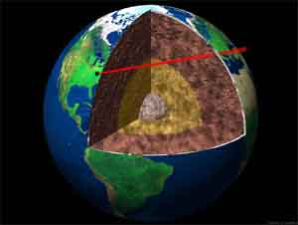
\includegraphics[width=7cm]{earthint}}

\vspace*{-1cm}

{\Huge \textcolor{yellow}{GLoBES}}
\end{center}

\vspace{1cm}

\begin{center}
Version from \today
\end{center}

%\end{titlepage}

%\title{}
%\date{}
%\author{}
%\maketitle

}

\clearpage
\thispagestyle{empty}
\bigskip
\begin{quote}
    Copyright \copyright  2004  The GLoBES Team.
    Permission is granted to copy, distribute and/or modify this document
    under the terms of the GNU Free Documentation License, Version 1.2
    or any later version published by the Free Software Foundation;
    with no Invariant Sections, no Front-Cover Texts, and no Back-Cover Texts.
    A copy of the license is included in the section entitled "GNU
    Free Documentation License".
\end{quote}
\bigskip
    


\cleardoublepage
\setcounter{page}{1}

\chapter*{What is \GLOBES ?}

\GLOBES\ (``General Long Baseline Experiment Simulator'') is a flexible
software package to simulate neutrino long baseline experiments. On the
one hand, it contains a comprehensive abstract experiment definition
language, which allows to describe most classes of long baseline experiments
at an abstract level. On the other hand, it provides a C-library to 
process the experiment information in order to obtain oscillation
probabilities, rate vectors, and $\Delta \chi^2$-values. Currently, 
\GLOBES\ is available for Linux. Since the source code is included,
the modifications to other operating systems should be doable.

\GLOBES\ allows to simulate experiments with stationary neutrino point sources, where each experiment is assumed to have only one neutrino source.
Such experiments are neutrino beam experiments and reactor experiments. 
Geometrical effects of a source distribution, such as in the sun or the 
atmosphere, can not be described. In addition, sources with a physically 
significant time dependencies  can not be studied, such as  supernov\ae. It 
is, however, possible to simulate beams with bunch structure, since the 
time dependence of the neutrino source is physically only important to suppress backgrounds. 

On the experiment definition side, either built-in neutrino fluxes
(\eg, neutrino factory) or arbitrary fluxes can be used. Similarly,
arbitrary cross sections, energy dependent efficiencies, the
energy resolution function, the considered oscillation channels, 
backgrounds, and many other features can be specified. 
For the systematics, energy
normalization and calibration errors can be simulated. Note that
the energy ranges and windows, as well as the bin widths can be
(almost) arbitrarily chosen, which means that variable bin
widths are allowed. Together with \GLOBES\ comes a number of
pre-defined experiments in order to demonstrate the capabilities
of \GLOBES\ and to provide prototypes for new experiments.

With the C-library, one can extract the $\Delta \chi^2$ for all defined 
oscillation channels for an experiment or any combination of experiments.
Of course, also low-level information, such as oscillation
probabilities or event rates, can be obtained. \GLOBES\ includes the
simulation of neutrino oscillations in matter with arbitrary matter 
density profiles, as well as it allows to simulate the matter density
uncertainty. As one of the most
advanced features of \GLOBES , it provides the technology to 
project the $\Delta \chi^2$, which is a function of all oscillation
parameters, onto any subspace of parameters by local minimization. 
This approach allows the inclusion of multi-parameter-correlations,
where external input (\eg, from solar parameters) can be imposed, too.
Applications of the projection mechanism include the projections onto the $\stheta$-axis and the $\stheta$-$\deltacp$-plane. In addition, all oscillation parameters can be kept free to precisely localize 
degenerate solutions.

\cleardoublepage
\tableofcontents

\cleardoublepage
\setcounter{page}{1}
\pagenumbering{arabic}

\chapter*{How to use this manual}
\addcontentsline{toc}{chapter}{How to use this manual}

As it is illustrated in \figu{GLOBES}, \GLOBES\ consists 
of several modules.
%
\begin{figure}[bht]
\begin{center}
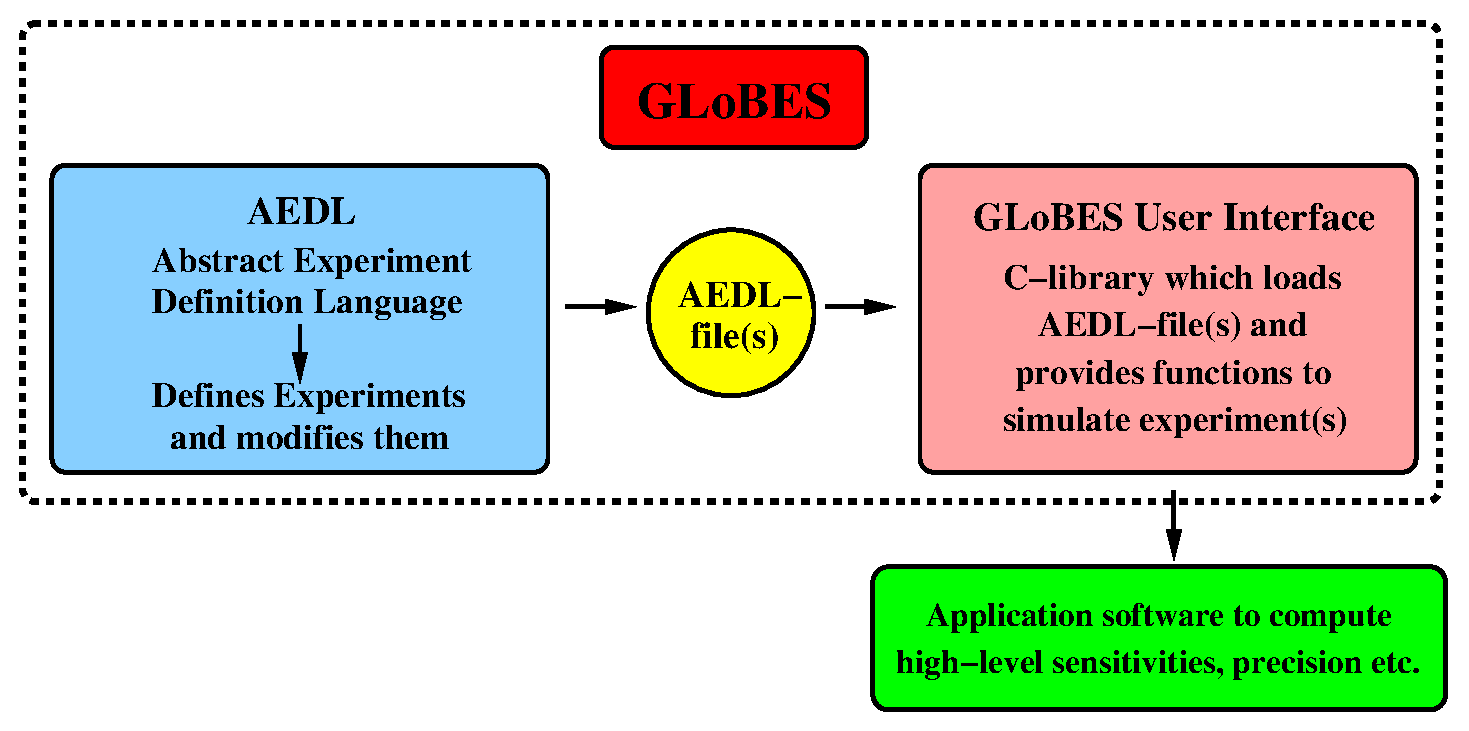
\includegraphics[width=16cm]{GLOBES}
\end{center}
\caption{\label{fig:GLOBES} Different modules in \GLOBES .}
\end{figure}
%
\AEDL (``Abstract Experiment Definition Language'') is a language
to define experiments in form of normal text files. One or more of 
the resulting \AEDL\ files can then be processed together with supporting 
flux or cross section files by the user interface. The user interface
is a C-library, which loads one or more \AEDL\ file(s)
containing the experiment definition(s). The user interface is linked 
against the application software, which calls the user interface functions
for the intended experiment simulation. 

The application 
software is, except from some example files, not part of \GLOBES , since
the evaluation of the experiment performance is often a matter of taste
and definition. In addition, the algorithms depend, especially for
high-precision instruments, very much on the oscillation parameters.
In general, it is quite simple to simulate superbeams and reactor
experiments. However, because of the more complicated topology, the
simulation of neutrino factories is much more difficult. In order
to demonstrate some of these difficulties, we show in this manual only
examples with neutrino factories. These examples can be found in
\Part~\ref{part:1} within the boxed pages. As complete files, they
are also available in the \GLOBES\ software package.

The \GLOBES\ software may have two target groups: 
Physicists, who are mainly interested in optimizing the potential
of specific experimental setups, and others, who are mainly
interested in the physics potential of different experiment types
from a theoretical point of view.
For the first group, \AEDL\ could be the most interesting aspect of
\GLOBES , where the user interface is only a tool to obtain specific
parameter sensitivities. In this case, \GLOBES\ could, serve as a
unified tool for the comparison and optimization of different experiment
 setups on equal footing, where
it is the primary objective to simulate the experiments as accurate
as possible. In addition, changes in experimental parameters, such as
efficiencies or the energy resolutions, can quickly be tested.
%
For the second user group, the pre-defined 
experiment definition files might already be sufficient to test
new conceptual approaches, and the user interface is the most interesting
aspect for sophisticated applications including correlations,
degeneracies, and multi-experiment setups. In either case, the \GLOBES\
software could serve as a platform for the exchange of experiment
definitions, and for an efficient splitting of work between
experimentalists and theorists.

The user interface functions are described in \Part~\ref{part:1} of 
this manual, which is the ``user's manual''. In there, first of all a 
short \GLOBES\ tour is given in \Chapt~\ref{chapter:tour} in order to 
have an overview over \GLOBES . 
After that, the user
interface is successively introduced from very basic to more sophisticated
function. Eventually, it is demonstrated how one can change many
experiment parameters at running time (such as baseline or target mass), and how one can obtain low-level
information. We recommend that everybody interested in \GLOBES\ should
become familiar at least with the concepts in \Chapt~\ref{chapter:tour}
 and some of the examples on the boxed pages. The examples can be 
 directly compiled 
 from the respective directory in the \GLOBES\ software package.

In \Part~\ref{part:2} of the manual, \AEDL\ is described. After an
introductory chapter, all functions are defined in greater detail.
This part might be more interesting for the experimental users who
want to modify or create \AEDL\ files. A useful tool in this context
is the software program ``globes'', which returns event rates and other
information for individual \AEDL\ files without further programming. 
For example, flux normalizations can with this tool be easily adjusted 
to reproduce the event rates of a specific experiment.

%Finally, \Part~\ref{part:3} of this manual serves as reference manual,
%and the appendix contains further supplementary information.

%%%%%%%%%%%%%%%%%%%%%%%%%%%%%%%%%%%
% PART I: User's manual
%%%%%%%%%%%%%%%%%%%%%%%%%%%%%%%%%%%

%%%%%%%%%%%%%%%%%%%%%%%%%%%%%%%%%%%
% PART I: User's manual
%%%%%%%%%%%%%%%%%%%%%%%%%%%%%%%%%%%

\part{User's manual}
\label{part:1}

\chapter{A short \GLOBES\ tour}
\label{chapter:tour}

To be written later: Short introduction such as ``With the following lines we obtain ...''
without detailed description of parameters. Should contain all most important functions of \GLOBES\ --
overview of main functions in \tabl{stdfunctions}.
Maybe: in form of long example which involves everything (for example: our famous bar plot, which involves
systematics, correlations, degeneracies and thus the full set of \GLOBES\ functions without being too
complicated in the application software part).

\begin{table}[t]
\begin{center}
\begin{tabular}{p{1.8cm}p{4.5cm}p{8.6cm}}
\hline
Function & Purpose & Parameters \ra\ Result \\
\hline
{\tt Chi} & $\chi^2$ with systematics only \newline (all initialized exps.) & ($\{ \theta_{12}, \theta_{13}, \theta_{23}, \deltacp , \sdm , \ldm, \hat{\rho_1},... , \hat{\rho_n} \}$)  \newline \ra\  $\chi^2$ \\[0.1cm]
{\tt SingleChi} & $\chi^2$ with systematics only \newline (only one experiment) & $(\{ \theta_{12}, \theta_{13}, \theta_{23}, \deltacp , \sdm , \ldm, \hat{\rho}_{N_{\mathrm{exp}}} \}, \, N_{\mathrm{exp}} )$   \newline \ra\ $\chi^2$ \\[0.1cm]
{\tt ChiTheta} & $\chi^2$ with systematics and correlations: Projection onto $\theta_{13}$-axis (all exps.) &  ($ \theta_{13}, \, \{ \theta_{12}, \theta_{23}, \deltacp , \sdm , \ldm, \hat{\rho_1}, ... , \hat{\rho_n} \}$) \newline \ra\  $\{ \chi^2, \theta_{12}, \theta_{23}, \deltacp , \sdm , \ldm, \hat{\rho_1}, ... , \hat{\rho_n} , N_{\mathrm{Iter}} \}$ \\[0.1cm]
{\tt Single-} \newline {\tt ChiTheta} & $\chi^2$ with systematics and correlations: Projection onto $\theta_{13}$-axis (one exp.) &  ($ \theta_{13}, \, \{ \theta_{12}, \theta_{23}, \deltacp , \sdm , \ldm,  \hat{\rho}_{N_{\mathrm{exp}}} \}, \, N_{\mathrm{exp}}$) \newline \ra\  $\{ \chi^2, \theta_{12}, \theta_{23}, \deltacp , \sdm , \ldm, \hat{\rho}_{N_{\mathrm{exp}}} , N_{\mathrm{Iter}} \}$ \\[0.1cm]
{\tt ChiDelta} & $\chi^2$ with systematics and correlations: Projection onto $\deltacp$-axis (all exps.) &  ($\deltacp, \, \{ \theta_{12}, \theta_{13}, \theta_{23},  \sdm , \ldm, \hat{\rho_1}, ... , \hat{\rho_n} \}$) \newline \ra\  $\{ \chi^2, \theta_{12}, \theta_{13}, \theta_{23}, \sdm , \ldm, \hat{\rho_1}, ... , \hat{\rho_n} , N_{\mathrm{Iter}} \}$ \\[0.1cm]
{\tt Single-} \newline {\tt ChiDelta} & $\chi^2$ with systematics and correlations: Projection onto $\deltacp$-axis (one exp.) &  ($ \deltacp, \, \{ \theta_{12}, \theta_{13}, \theta_{23}, \sdm , \ldm,  \hat{\rho}_{N_{\mathrm{exp}}}  \}, \, N_{\mathrm{exp}}$) \newline \ra\  $\{ \chi^2, \theta_{12}, \theta_{13}, \theta_{23},  \sdm , \ldm, \hat{\rho}_{N_{\mathrm{exp}}} , N_{\mathrm{Iter}} \}$ \\[0.1cm]
{\tt ChiTheta-} {\tt Delta} & $\chi^2$ with systematics and correlations: Projection onto $\deltacp$-$\theta_{13}$-plane (all exps.) &  ($\theta_{13}, \, \deltacp, \, \{ \theta_{12}, \theta_{23},  \sdm , \ldm,  \hat{\rho_1}, ... , \hat{\rho_n} \}$) \newline \ra\  $\{ \chi^2, \theta_{12}, \theta_{23}, \sdm , \ldm,  \hat{\rho_1}, ... , \hat{\rho_n} , N_{\mathrm{Iter}} \}$ \\[0.1cm]
{\tt SingleChi-} {\tt Theta- } {\tt Delta} & $\chi^2$ with systematics and correlations: Projection onto $\deltacp$-$\theta_{13}$-plane (one exp.) &  ($ \theta_{13}, \, \deltacp, \, \{ \theta_{12}, \theta_{23}, \sdm , \ldm,  \hat{\rho}_{N_{\mathrm{exp}}} \}, \, N_{\mathrm{exp}}$) \newline \ra\  $\{ \chi^2, \theta_{12},  \theta_{23},  \sdm , \ldm, \hat{\rho}_{N_{\mathrm{exp}}} , N_{\mathrm{Iter}} \}$ \\[0.1cm]
{\tt ChiNP} & $\chi^2$ with systematics and correlations: Projection onto $N$-parameter hyper-plane (one exp.) & ??? to be defined \\[0.1cm]
{\tt Single-} {\tt ChiNP} & $\chi^2$ with systematics and correlations: Projection onto $N$-parameter hyper-plane (one exp.) & ??? to be defined \\[0.1cm]
{\tt ChiAll} & Lokal minimum of $\chi^2$ with respect to all parameters (all exps.) &
($ \{ \theta_{13}, \theta_{12}, \theta_{23}, \deltacp , \sdm , \ldm,  \hat{\rho_1}, ... , \hat{\rho_n} \}$) \newline \ra\  $\{ \chi^2, \theta_{13}, \theta_{12}, \theta_{23},$ \newline \hspace*{1.4cm} $ \deltacp , \sdm , \ldm,  \hat{\rho_1}, ... , \hat{\rho_n} , N_{\mathrm{Iter}} \}$ 
\\[0.1cm]
{\tt Single-} {\tt ChiAll} & Lokal minimum of $\chi^2$ with respect to all parameters (one exp.) &  ($ \{ \theta_{13}, \theta_{12}, \theta_{23}, \deltacp , \sdm , \ldm,  \hat{\rho}_{N_{\mathrm{exp}}} \}, \, N_{\mathrm{exp}}$) \newline \ra\  $\{ \chi^2, \theta_{13}, \theta_{12}, \theta_{23}, \deltacp , \sdm , \ldm, \hat{\rho}_{N_{\mathrm{exp}}} , N_{\mathrm{Iter}} \}$ \\[0.1cm]
\hline
\end{tabular}
\end{center}
\caption{\label{tab:stdfunctions} \index{Standard functions (table)} The \GLOBES\ standard function to obtain a $\chi^2$-value for all or one of the initialized experiments. The curly brackets refer to the parameters to be transferred in form of a list. The parameter $\hat{\rho}_i \equiv \rho_i/\bar{\rho}_i$ refers to the matter density scaling factor, which is $1.0$ for leaving the matter density profile unchanged. Note that all functions but {\tt Chi} and {\tt SingleChi} are using minimizers which have to be initialized with {\tt SetInputErrors} and {\tt SetStartingValues} first.}
\end{table}

\chapter{Getting started with \GLOBES }

In this first chapter of the user's manual, we assume that the \GLOBES\ software is readily installed on your computer system. We demonstrate how to load pre-defined experiments and re-obtain information about them. However, we only secondarily discuss the usage of \GLOBES\ in your specific programming language, such as C, Mathematica, or others. Thus, you should be familiar of how to load \GLOBES\ on your computer system before reading this chapter. An example of how to use \GLOBES\ with C can be found on page~\pageref{ex:c}. 

\example{Using \GLOBES\ with C}{\label{ex:c}
\index{C-Code}

Here comes some complete C-code with a very simple example of how to use \GLOBES .
 
}

\begin{table}[t]
\begin{center}
\begin{tabular}{lll}
\hline
Quantities & Examples & Units \\
\hline
Angles & $\theta_{13}$, $\theta_{12}$, $\theta_{23}$, $\deltacp$ & Radians  \\
Mass squared differences & $\sdm$, $\ldm$ & $\mathrm{eV}^2$ \\
Matter densitities & $\rho_i$ & $\mathrm{g}/\mathrm{cm}^3$ \\
Baseline lengths & $L_i$ & $\mathrm{km}$ \\
Energies & $E_\nu$ & $\mathrm{GeV}$ \\  
Fiducial masses & $m_{\mathrm{Det}}$ & $\mathrm{kt}$ \\
Time intervals & $t_{\mathrm{run}}$ & $\mathrm{yr}$ \\
Source powers & $P_{\mathrm{Source}}$ & ??? \\
% Integrated luminosities & $m_{\mathrm{Det}} \, t_{\mathrm{run}}$ & $\mathrm{kt \cdot yr}$ \\
Cross sections & $\sigma_{\mathrm{CC}}$ &  ???? \\
\hline
\end{tabular}
\mycaption{\label{tab:units} \index{Units in \GLOBES } Quantities used in \GLOBES , examples of these quantities, and their standard units in the application software.}
\end{center}
\end{table}

Throughout the programming interface of \GLOBES , the software needs to transfer parameters to and from the software core. Unless the Experiment Definition Module \EDM , the programming interface only uses one set of units for each type of quantity in order to avoid confusion about the definition of individual parameters. \tabl{units} summarizes the units of the most important quantities used in \GLOBES .

\begin{table}[t]
\begin{center}
\begin{tabular}{llp{7cm}c}
\hline
Experiment & Filename & Short description & Refs. \\
\hline 
\multicolumn{3}{l}{\underline{Conventional beams:}} \\
??? & & \\[0.1cm]

\multicolumn{3}{l}{\underline{First-generation superbeams:}} \\
\JHFSK\ ($\nu$) & {\tt JHFSK.exp} & JHF (J-PARC) to Super-Kamiokande, neutrino running &  \cite{Huber:2002mx,Huber:2002rs} \\
\JHFSK\ ($\bar\nu$)& {\tt JHFSKanti.exp} & JHF (J-PARC) to Super-Kamiokande, antineutrino running &  \cite{Huber:2002rs} \\
\NUMI\  ($\nu$), OA $9 \, \mathrm{km}$ & {\tt NUMI9.exp} & NuMI with off-axis angle of $9 \, \mathrm{km}$ for $L=712 \, \mathrm{km}$, neutrino running & \cite{Huber:2002rs} \\
\NUMI\  ($\bar{\nu}$), OA $9 \, \mathrm{km}$ & {\tt NUMI9anti.exp} & NuMI with off-axis angle of $9 \, \mathrm{km}$ for $L=712 \, \mathrm{km}$, antineutrino running & \cite{Huber:2002rs} \\
\NUMI\  ($\nu$), OA $12 \, \mathrm{km}$ & {\tt NUMI12.exp} & NuMI with off-axis angle of $12 \, \mathrm{km}$ for $L=712 \, \mathrm{km}$, neutrino running & \cite{Huber:2002rs} \\
\NUMI\  ($\bar{\nu}$), OA $12 \, \mathrm{km}$ & {\tt NUMI12anti.exp} & NuMI with off-axis angle of $12 \, \mathrm{km}$ for $L=712 \, \mathrm{km}$, antineutrino running & \cite{Huber:2002rs} \\
\SPL\  ($\nu$) & {\tt SPL.exp} & SPL (CERN), neutrino running &  ??? \\
\SPL\  ($\bar\nu$) & {\tt SPLanti.exp} & SPL (CERN), antineutrino running & ??? \\[0.1cm]
 
\multicolumn{3}{l}{\underline{Superbeam upgrades:}} \\
\JHFHK\ ($\nu$) & {\tt JHFHK.exp} & JHF (J-PARC) to Hyper-Kamiokande superbeam upgrade, neutrino running &  \cite{Huber:2002mx,Huber:2002rs} \\
\JHFHK\ ($\bar\nu$)& {\tt JHFHKanti.exp} & JHF (J-PARC) to Hyper-Kamiokande superbeam upgrade, antineutrino running &  \cite{Huber:2002mx,Huber:2002rs} \\[0.1cm]

\multicolumn{3}{l}{\underline{Neutrino factories:}} \\
\NuFactI\ & {\tt NuFact.exp} & Initial stage neutrino factory, symmetric operation in both polarities & \cite{Huber:2002mx} \\
\NuFactII\  & {\tt NuFact2.exp} & Advanced stage neutrino factory, symmetric operation in both polarities & \cite{Huber:2002mx,Huber:2003ak} \\[0.1cm]

\multicolumn{3}{l}{\underline{Reactor experiments:}} \\
\ReactorI\ & {\tt Reactor.exp} & Small reactor experiment with identical near and far detectors & \cite{Huber:2003pm} \\
\ReactorII\ & {\tt Reactor2.exp} & Large reactor experiment with identical near and far detectors & \cite{Huber:2003pm} \\[0.1cm]

\multicolumn{3}{l}{\underline{$\beta$-Beams:}} \\
\Beta\ ($\nu$) & {\tt BETA.exp} & $\beta$-Beam, neutrino running & ??? \\
\Beta\ ($\bar\nu$) & {\tt BETAanti.exp} & $\beta$-Beam, antineutrino running & ??? \\
\hline
\end{tabular}
\end{center}
\mycaption{\label{tab:experiments} \index{Experiment data files (table)} Different pre-defined experiments, their filenames (to be used in {\tt LoadExperiment}), their short description, and the references in which they are defined. Note that all experiments use in their standard configurations one year of running time. Details about the experiment parameters can be obtained with {\tt InfoExperiment}(Experiment number) after they have been loaded.}
\end{table}

In principle, \GLOBES\ can handle any number of different long-baseline experiments simultaneously. This means that their $\chi^2$-values are added {\em after} the minimization over the independent systematics parameters and {\em before} any minimization over the oscillation parameters. Though the simplest case of only one experiment may be most often used, more experiments are useful in many cases. For example, running a superbeam some years in the neutrino mode and some years in the antineutrino mode can be, to a first approximation, simulated by the combination of two such experiments.\footnote{Note that in this case the systematics parameters are minimized over independently, which means that this approach does not allow correlations among the systematics parameters. Therefore, the neutrino factory with the symmetric operation of both polarities is encapsulated into a single experiment.} Another example is the test of synergetic effects among different experiment types. Thus, \GLOBES\ has an internal (initially empty) list of currently initialized experiments. To add a pre-defined experiment to this list, one can use the function {\tt LoadExperiment}:
\begin{function}
\index{{\tt LoadExperiment}}
\index{Experiment initialization}
{\tt LoadExperiment}$($``filename'' $)$ adds a single experiment to the list of currently loaded experiments. All currently loaded experiments are evaluated simultaneously (if not explicitely stated otherwise), \ie , their $\chi^2$-values are added.
\end{function}
A list of pre-defined experiment types, their filenames, their short descriptions, and the references of their definitions can be found in \tabl{experiments}. To remove all experiments from the evaluation list, one uses {\tt ClearExp}:
\begin{function}
\index{{\tt ClearExp}}
{\tt ClearExp}$()$ removes all experiments from the evaluation list.   
\end{function}
Both functions do not return anything. Thus, one can either add an experiment to the internal evaluation list, or remove all experiments from this list. After adding an experiment, it gets an internal experiment number $N_{\mathrm{exp}}$ assigned in the order of the addition, which is starting from zero and running to the number of experiments minus one. Therefore, one will be able to access the individual experiment by its number later.

Since the pre-defined experiments in \tabl{experiments} are given for one year running time, specific target masses, and specific source powers, it is useful to change these parameters of the individual experiments:
\begin{function}
\index{{\tt SetRunningTime}}
{\tt SetRunningTime}$(N_{\mathrm{exp}},t_{\mathrm{run}})$ sets the running time of experiment number $N_{\mathrm{exp}}$ to $t_{\mathrm{run}}$ years.
\end{function}
 \begin{function}
\index{{\tt SetTargetMass}}
{\tt SetTargetMass}$(N_{\mathrm{exp}},m_{\mathrm{Det}})$ sets the fiducial mass of experiment number $N_{\mathrm{exp}}$ to $m_{\mathrm{Det}}$ kilotons.
\end{function}
\begin{function}
\index{{\tt SetSourcePower}}
{\tt SetSourcePower}$(N_{\mathrm{exp}},P_{\mathrm{Source}})$ sets the source power of experiment number $N_{\mathrm{exp}}$ to $P_{\mathrm{source}}$. The definition of the source power depends on the experiment type: ... (MISSING).
\end{function}
Thus, these functions also demonstrate how to use the assigned experiment number.

A useful function to re-obtain the information about the initialized experiments is the function {\tt InfoExperiment}:
\begin{function}
\index{{\tt InfoExperiment}}
{\tt InfoExperiment}$()$ prints a list of the initialized functions with their experiment numbers and their most important parameters to the standard output.
\end{function} 
Especially, after changing individual parameters, such as baseline or target mass, this information can be useful to check the changes. Another useful function is {\tt ShowChannels}, which prints the initialized oscillation channels for a specified experiment:
\begin{function}
\index{{\tt ShowCannels}}
{\tt ShowChannels}$(N_{\mathrm{exp}})$ prints the information about the oscillation channels of the experiment with the number $N_{\mathrm{exp}}$ to the standard output.
\end{function}

Compared to an existing experiment, which uses real data, a future experiment uses simulated data. Thus, the {\em true parameter values} and their results in form of the reference rate vectors are simulated. After setting the true parameter values, the {\em fit parameter values} can be varied in order to obtain information on the measurement performance for the given set of true parameter values. Therefore, it is often useful to show the results of a future measurement as function of the true parameter values for which the reference rate vectors are computed -- at least within the currently allowed ranges. The true parameter values for the vacuum neutrino oscillation parameters have to be set by the functions {\tt SetVacuumParameters} and {\tt SetRates} {\em before} any evaluation function is used and {\em after} the experiments have been initialized and the experiment parameters have been adjusted which could change the rates (such as baseline or target mass). Any matter effects are then included automatically depending on the experiment definitions.
\begin{function}
\index{{\tt SetVacuumParameters}}
{\tt SetVacuumParameters}$(\{\theta_{12}, \theta_{13}, \theta_{23}, \deltacp , \sdm , \ldm \})$ sets the neutrino oscillation parameters to be used to compute the reference rate vector in vacuum.
\end{function}
\begin{function}
\index{{\tt SetRates}}
{\tt SetRates}$( )$ computes the reference rate vector for the neutrino oscillation parameters set with {\tt SetVacuumParameters}. 
\end{function}
Finally, an initialization sequence for \GLOBES\ could look like this:
\begin{quote}
{\tt
ClearExp(); \\
InitExperiment("JHFHK.exp"); \\
SetRunningTime(0, 2.0); \\
InitExperiment("JHFHKanti.exp"); \\
SetRunningTime(1, 6.0);\\
MInfoExperiment(); \\
SetVacuumParameters(\{0.55, 0.16, 3.14/4, 3.14/2, 7e-5, 2e-3\}); \\
SetRates();
} 
\end{quote}
This piece of code initializes the JHF (J-PARC) to Hyper-Kamiokande superbeam upgrade with two years of neutrino running and six years of antineutrino running, \ie, an overall running time of eight years. The final configuration is then printed to the standard output and the reference rate vector is set to the chosen parameter values.

\chapter[Calculating $\chi^2$ with systematics only]{Calculating $\boldsymbol{\chi^2}$ with systematics only}

\index{Systematics}
Calculating a $\chi^2$-value with or without systematics, but no correlations and degeneracies, is the simplest and fastest possibility to obtain high-level information on an experiment. I general, \GLOBES\ uses the six independent oscillation parameters $\theta_{12}$, $\theta_{13}$, $\theta_{23}$, $\deltacp$, $\sdm$, $\ldm$, as well as the matter density of each experiment. Thus, there are six plus the number of experiments parameters determining the rate vectors. Using the matter densities in addition to the oscillation parameters will allow the simulation of matter density uncertainties: In this approach, the matter densities can be treated as parameters to be measured by the experiments within certain limits, where the limits are given by the observed precision of the matter density profile. Defining a independent matter density for each experiment is necessary if the baselines are completely uncorrelated. For correlated or even identical baselines, one may rather want to encapsulate the experiments into a single experiment definition. 

\example{Correlation between $\stheta$ and $\deltacp$}{
\label{ex:corrth13dcp}

\index{Two-parameter correlation}
A typical application for {\tt Chi} and {\tt SingleChi} is the visualization of two-parameter correlations. For example, to show the correlation between $\stheta$ and $\deltacp$ at a large neutrino factory with four years of running time for each polarity, one can use the following code:
\begin{quote}
{\tt
/\% Experiment initialization: \%/ \\
ClearExp(); \\
 InitExperiment("{\tt NuFact2.exp}"); \\
 SetRunningTime(0,4.0); \\
 MInfoExperiment(); \\
\\
/\% Set reference rate vector: \%/ \\
th12=arcsin(sqrt(0.8))/2; sdm=7e-5; \\
th23=3.14/4; ldm=2e-3; \\
th13=arcsin(sqrt(0.001))/2; dcp=3.14/2; \\
\mbox{SetVacuumParameters(\{th12, \, th13, \, th23, \, dcp, \, sdm, \, ldm\}); }\\
 SetRates(); \\
\\
/\% Compute chi-square matrix: \%/ \\
for (float x=-4; x<-2; x=x+2/50) \\
\hspace*{0.5cm} for (float y=0; y<200; y=y+200/50) \{ \\
\hspace*{1cm} theth13 = arcsin(sqrt(10$\hat{\, \, \,}$x))/2; \\
\mbox{\hspace*{1cm} Print(\{x,y,Chi(\{th12, theth13,  th23,  y, sdm, ldm, 1.0\}) \}) \};}
}
\end{quote}

The resulting matrix can then be plotted as a contour plot (2 d.o.f.):
\begin{center}
\colorbox{white}{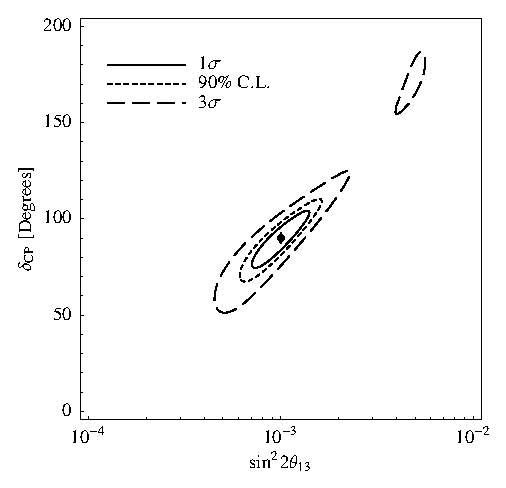
\includegraphics[width=8cm]{correx}}
\end{center}

}

Keeping all oscillation parameters and matter densities fixed, one can use the following functions to obtain the total $\chi^2$ of all specified oscillation channels including systematics:
\begin{function} 
\index{{\tt Chi}}
{\tt Chi}$(\{ \theta_{12}, \theta_{13}, \theta_{23}, \deltacp , \sdm , \ldm, \hat{\rho_1}, \hdots , \hat{\rho_n} \})$  returns the total added $\chi^2$ of all loaded experiments.
\end{function}
\begin{function}
\index{{\tt SingleChi}}
 {\tt SingleChi}$(\{ \theta_{12}, \theta_{13}, \theta_{23}, \deltacp , \sdm , \ldm, \hat{\rho}_{N_{\mathrm{exp}}} \}, \, N_{\mathrm{exp}} )$  returns the total $\chi^2$ of the experiment number $N_{\mathrm{exp}}$.
\end{function}
Note that the result of {\tt Chi} corresponds to the sum of all of the {\tt SingleChi}'s of the loaded experiment. This equality will not hold for the minimizors in the next sections anymore. In both functions, one has to give the matter density scaling factor $\hat{\rho_i}$ for each of the used experiments. The effect of this scaling factor depends on the type of the matter density profile, which is given in the  experiment definition. For a constant matter density, it is simply the ratio of the matter density and the average matter density specified in the experiment definition, \ie , $\hat{\rho_i} \equiv \rho_i/\bar{\rho}_i$.\index{Matter scaling factor} For a matter density profile, it is an overall scaling factor: The matter density in each layer is multiplied by this factor. In most cases one wants to take a scaling factor of $1.0$ here, which simply means taking the matter density profile as it is given in the experiment definition. Moreover, note that its effect is in general small for short baselines. An example of how to use  {\tt Chi} (or {\tt SingleChi}) can be found on page~\pageref{ex:corrth13dcp}.  

\index{Systematics}
The treatment of systematics is done by the usage of auxiliary systematics parameters, which are taken completely uncorrelated among different oscillation channels, and treated with simple Gaussian statistics. One such example is the signal normalization error, \ie, an error to the overall normalization of the signal. For illustration, we assume that the signal event rate in the $i$th bin $s_i^0$ of one oscillation channel is altered by the overall normalization auxiliary parameter\index{Auxiliary parameter} of this channel, \ie , 
\be
 s_i = s_i(n_s) = s_i^0 \cdot (1 + n_s),
\ee
where $n_s$ is the signal normalization parameter. The total number of events in the $i$th bin $x_i$ also includes the background event rates $b_i$, \ie, $x_i = s_i + b_i$, which may have their own systematics parameters.
In order to implement an overall signal normalization error $\sigma_{n_s}$,  the $\chi^2$, which includes all event rates $x_i$ of all bins, is minimized over the auxiliary parameter $n_s$:
\be
 \hat{\chi^2} = \underset{n_s}{\mathrm{min}} \left(  \chi^2(n_s, \hdots) + \frac{(n_s)^2}{\sigma_{n_s}^2} \right).
\ee 
This minimization is done independently for all auxiliary parameters of this oscillation channel. The total $\chi^2$ for the considered experiment is finally obtained by repreating this procedure for all oscillation channels and adding their $\chi^2$-values. In general, the situation is more complicated because of the usage of many systematical errors. More details about systematics parameters and the definition of signal, background, and oscillation channels can be found in the \EDM\ part of this book, too.

The systematics minimization of an experiment can be easily switched on and off, \ie, one can also compute the $\chi^2$ without even taking into account systematics:
\begin{function}
\index{{\tt SetSystematics}}
{\tt SetSystematics}$(N_{mathrm{exp}}, \, sys)$ switches the systematics minimization for experiment $N_{\mathrm{exp}}$ on (sys=1) or off (sys=0).
\end{function}
This function can be especially useful for the test of the impact of systematics.
??? Wie einzelne Systematik-Parameter ein und ausschalten? Sonst individuell nicht testbar! ??? Verweis auf appendix? 

\chapter[Calculating $\chi^2$-projections: how one can include correlations]{Calculating $\boldsymbol{\chi^2}$-projections: how one can include correlations}

\index{Multi-parameter correlation}
This chapter deals with the rather complicated issue of $n$-parameter correlations. Since it has before this software  not been possible to include the full $n$-parameter correlations in the high-dimensional parameter space with reasonable effort, it is the core part of this software  -- as well as its strength. Of course, calculating $\chi^2$-projections is somewhat more complicated than using systematics only. Therefore, we use a simple step by step introduction to the problem. 

\section{Introduction}

\index{Projection of manifold}
In principle, the precision of an individual parameter measurement including correlations can be obtained as the projection of the $n$-dimensional fit manifold onto the respective axis. Similarly, one can project the fit manifold onto a plane, such as the $\stheta$-$\deltacp$-plane, if one wants to explicitely show this correlation with all the other parameter correlations included. In practice, this projection is very difficult: a grid-based method would need $(N_{\mathrm{grid}})^n$ function calls of {\tt Chi} or {\tt SingleChi} to calculate the precision including the full $n$-parameter correlation, where $N_{\mathrm{grid}}$ is the number of points in each direction of the lattice. For example, taking only $N_{\mathrm{grid}}=20$ and $n=7$ (six oscillation parameters and matter density) would mean more than one billion function calls of {\tt Chi} or {\tt SingleChi}. One can easily image that this is too much for any sophisticated application.

\index{Minimizer}
The solution to this problem is using a local $n$-dimensional minimizer instead of a grid-based method. It turns out that such a minimizer can include a full $6$-parameter correlation with of the order of $1\, 000$ function calls of {\tt Chi} or {\tt ChiNew}. It is a standard method which can be found in every good book for standard numerical calculation routines. Thus, for each point on the projection axis/plane, one can obtain a result within about $10$ to $30$ seconds on a modern computer, which means that the complete measurement precision for one fixed true parameter set can be obtained in as much as $10$ to $15$ minutes. One can easily imagine that such a minimizer makes more sophisticated applications possible with the help of overnight calculations, such as showing the dependencies on the true parameter values.

This approach also has a major disadvantage: One can not simply program a robust grid-based code and let it run, since using a local minimizer always means that one may end up in an unwanted local minimum and not in the investigated one. Thus, one has to use some (analytical or numerical) knowledge on the topology of the fit manifold and start the local minimizer close enough to the investigated solution. Fortunately, this can be done quite straightfoward in most cases, since the structure of the neutrino oscillation formulas does not cause very complicated topologies of the fit manifolds. Especially, the are plenty of analytical discussions of this issue, which means that one can implicitely use this knowledge to obtain better predictions for the measurement performances. Note that, since one can easily find the global fit minimum at the best-fit values, any solution found with the local minimizer makes the measurement performance worse. Thus, one can only run the danger to obtain a too optimistic solution if one does not find the other local minima below the chosen confidence level.

\index{Priors} \index{Input errors} \index{Starting values}
In many cases, the fit manifold is restricted by the knowledge from earlier experiments. For example, the knowledge on the solar parameters will in most cases be supplied by the solar neutrino experiments. If the external precision of a parameter is at the time of the measurement better than the one of the experiment itself, one has to impose some external knowledge on this parameter. This external knowledge may reduce the $n$-dimensional fit manifold in the respective direction. In the most extreme case, keeping all parameters but the measured one fixed in the analysis means that all parameters are determined externally with infinitively high precisions. Thus, using the projection method on the axis/plane of interest is a reasonable approach. The inclusion of external input in \GLOBES\ is done by the use of Gaussian {\em priors}: We assume that an external measurement has determined the measured parameter to be at the central value (called {\em starting value}) with a $1 \sigma$ Gaussian error (called {\em input error}). The explicit definition of these priors will be shown in the next section.

\section{The treatment of external input}
\label{sec:externalinput}

\index{External input}
It is one of the strengths of the \GLOBES\ software to use external input to reduce the fit manifold with the knowledge from external (eariler) measurements. The treatment of external input is done by the addition of Gaussian {\em priors} to the final\footnote{After the systematics minimization and after all $\chi^2$'s are added for all channels} $\chi^2$-function  and the minimization over the respective parameters. For example, for the matter density, one obtains as the minimized $\chi^2_F$ after minimzation over $\rho$
\be
 \chi^2_F = \underset{\rho}{\mathrm{min}} \left( \chi^2(\rho) + \frac{(\rho - \rho^0)^2}{\sigma_\rho^2} \right).
\label{equ:priors}
\ee
In practice, this minimzation is done simultaneously over all priors and free oscillation parameters, but this example serves as a very simple illustration. In \equ{priors}, $\rho^0$ is the {\em starting value} of the prior, and $\sigma_\rho$ the $1 \sigma$ absolute {\em input error}. Thus, it is assumed that an external measurement has determined the matter density with a precision (input error) $\sigma_\rho$ at the central value $\rho^0$. Usually, the starting value corresponds to the best-fit value and the input error to the $1 \sigma$ half width of the external measurement. For the matter density, $\rho^0$ can be set to the average matter density $\bar{\rho}$ and $\sigma_\rho$ to the matter density uncertainty. Since \GLOBES\ may also use a matter density profile, it actually uses a scaling factor $\hat\rho$ instead of the average matter density (see last section), \ie, $\rho^0=1.0$ is the central value in either case. Thus, $\sigma_\rho$ directly correponds to the uncertainty of this scaling factor. For instance, using the PREM (``Preliminary Reference Earth Model'') profile, $\rho^0 = 1.0$ and $\sigma_\rho = 0.05$ is a conservative estimate of the PREM profile uncertainty.  \index{PREM profile}

In principle, one can set the priors for the matter density and all oscillation parameters. For example, if the disappearance channels of the experiment determine the leading oscillation parameters, once can set very large values for the input errors ($\sigma$'s). If, however, earlier external measurements provide better information, one can set their absolute precisions with the input errors. The starting values are usually set to the best-fit values. In some cases, it may be necessary to adjust them, such as for $\ldm$ and the negative mass hierarchy to $\rho^0_{\ldm} = - |\ldm|$ if some external precision on $| \ldm |$ is imposed and one is investigating the negative-sign solution. In other cases, minor modifications of the starting values can cause a faster convergence of the algorithm.
In either case, two function have to be called {\em before the usage of any minimizer}:
\begin{function}
\index{{\tt SetStartingValues}}
{\tt SetStartingValues}$(\{\rho^0_{\theta_{12}}, \, \rho^0_{\theta_{13}}, \, \rho^0_{\theta_{23}}, \, \rho^0_{\deltacp}, \, \rho^0_{\sdm}, \, \rho^0_{\ldm}, \, \rho^0_{\hat\rho} \})$ sets the starting values for all of the following minimizer calls.
\end{function}
\begin{function}
\index{{\tt SetInputErrors}}
{\tt SetInputErrors}$(\{\sigma_{\theta_{12}}, \, \sigma_{\theta_{13}}, \, \sigma_{\theta_{23}}, \, \sigma_{\deltacp}, \, \sigma_{\sdm}, \, \sigma_{\ldm}, \, \sigma_{\hat\rho} \})$ sets the input errors for all of the following minimizer calls.
\end{function}
Both functions may take one matter density parameter or as many as there are experiments. Since the assumptions about the matter density profile are usually similar for the loaded experiments, using only one matter density parameter is a useful tool to apply the same starting value  and input error to all loaded experiments.
Eventually, a typical initialization of the external input may look like this:
\begin{quote}
{\tt
SetStartingValues(\{th12, th13, th23, dcp, sdm, ldm, 1.0\}); \\
SetInputErrors(\{th12*0.1, 10, 10, 10, sdm*0.1, ldm, 0.05\}); 
}
\end{quote}
In this example, the starting values are set to the best-fit values. The input errors for $\theta_{13}$, $\theta_{23}$, $\deltacp$, and $\ldm$ are kept large, since the experiment measures these parameters itself. However, some precision on $\ldm$ is imposed to avoid ending up in the negative-sign solution. The solar parameters $\theta_{12}$ and $\sdm$ are assumed to be known with $10\%$ precision each.\footnote{In fact, accelerator-based long-baseline experiments are only sensitive to the product $\sin 2 \theta_{12} \cdot \sdm$, which means that these errors effectively add up to an error of this product.} Finally, the matter density uncertainties are assumed to have an amplitude of $5\% \,  \bar\rho$.
 
\example{Projection of two- and $n$-dimensional manifold onto $\stheta$-axis}{
\label{ex:corrproj}
\index{Projection of manifold}
\index{Two-parameter correlation}
\index{Multi-parameter correlation}

This example demonstrates how to use  {\tt ChiTheta} to project the fit manifold onto the $\stheta$-axis, \ie, how one can include correlations. We compute two sets of data: one for keeping all parameters but $\deltacp$ fixed (two-parameter correlations), and one for keeping all parameters free (multi-parameter correlation), but some external input for the solar parameters and $\rho$. Note that fixing all parameters but $\deltacp$ corresponds to imposing external knowledge on these parameters.

\begin{quote}
{\tt {\footnotesize
/\% Experiment initialization, set reference rate vector: \%/ \\
\mbox{ClearExp(); InitExperiment("{\tt NuFact2.exp}"); SetRunningTime(0,4.0); }\\
th12=arcsin(sqrt(0.8))/2; sdm=7e-5; th23=3.14/4; ldm=2e-3; \\
th13=arcsin(sqrt(0.001))/2; dcp=3.14/2; \\
\mbox{SetVacuumParameters(\{th12, th13, th23, dcp, sdm, ldm\}); SetRates();}\\
\\
/\%  Compute chi-square list with all but dcp fixed: \%/ \\
SetStartingValues(\{th12, th13, th23, dcp, sdm, ldm, 1.0\}); \\
\mbox{SetInputErrors(\{th12*0.001, 10, th23*0.001, 10, sdm*0.001, ldm*0.001, 0.001\});} \\
for (float x=-4; x<-2; x=x+2/20) \\
\mbox{\hspace*{0.5cm} Print(\{x,ChiDelta(x,\{th12, th13, th23, dcp, sdm, ldm, 1.0\}) \}); }\\
\\
/\% Compute chi-square list with all parameters free: \%/ \\
\mbox{/\% (but: 10\% prec. for solar params, 5\% for matter density) \%/} \\
SetStartingValues(\{th12, th13, th23, dcp, sdm, ldm, 1.0\}); \\
SetInputErrors(\{th12*0.1, 10, 10, 10, sdm*0.1, ldm, 0.05\}); \\
for (float x=-4; x<-2; x=x+2/20) \\
\mbox{\hspace*{0.5cm} Print(\{x,ChiDelta(x,\{th12, th13, th23, dcp, sdm, ldm, 1.0\}) \});}
}}
\end{quote}
The two lists of data then represent the $\stheta$ precisions with two-parameter correlations (gray-shaded) and multi-parameter correlations (arrows):
\begin{center}
\colorbox{white}{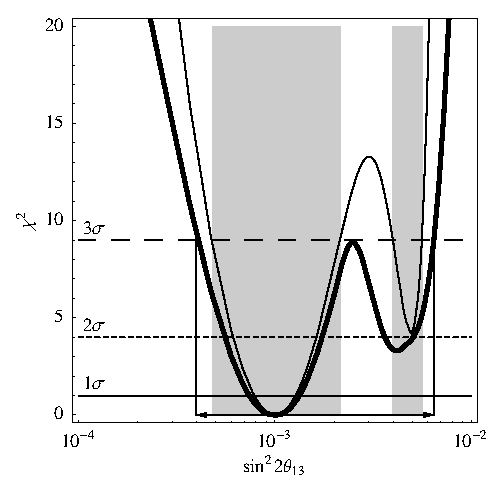
\includegraphics[width=6cm]{projallex}}

\vspace*{0.1cm}

\footnotesize{(Same parameters as on page~\pageref{ex:corrth13dcp} and in \figu{projex}, but 1 d.o.f.)}
\end{center}
}

\section[Projection onto the $\stheta$-axis or $\deltacp$-axis]{Projection onto the $\boldsymbol{\stheta}$- or $\boldsymbol{\deltacp}$-axis}
\index{Projection onto axis}

\begin{figure}[t]
\begin{center}
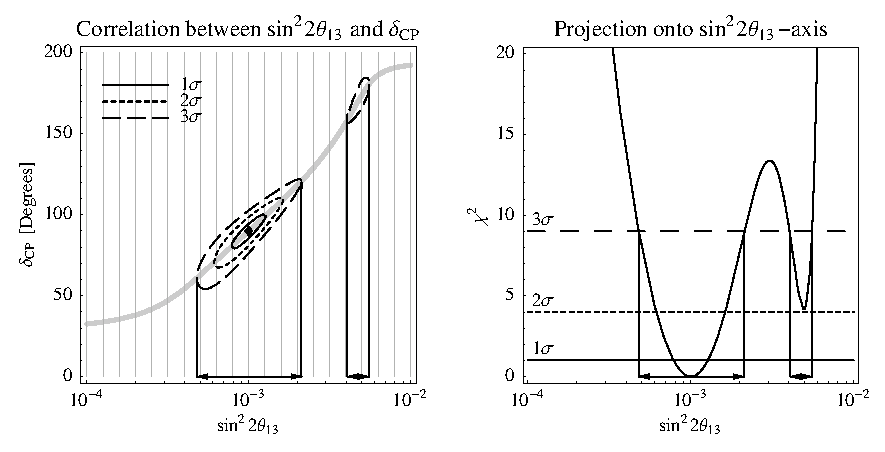
\includegraphics[width=16cm]{projex}
\end{center}
\mycaption{\label{fig:projex} Left plot: The correlation between $\stheta$ and $\deltacp$ as calculated in the example on page~\pageref{ex:corrth13dcp}, but for 1 d.o.f. only. Right plot: The $\chi^2$-value of the projection onto the $\stheta$-axis as function of $\stheta$. The projection onto the  $\stheta$-axis is obtained by finding the minimum $\chi^2$-value for each fixed value of $\stheta$ in the left-hand plot, \ie, along the gray vertical lines. The thick gray curve marks the position of these minima in the left-hand plot. The arrows mark the obtained fit ranges for $\stheta$ at the $3 \sigma$ confidence level (1 d.o.f.), \ie , the precision of $\stheta$.}
\end{figure}

The projection onto the $\stheta$- (or $\deltacp$-) axis is performed by fixing $\stheta$ (or $\deltacp$) and minimizing the $\chi^2$-function over all free fit parameters and the matter densities. We illustrate this method at the example of the projection of the two-dimensional manifold in the $\stheta$-$\deltacp$-plane onto the $\stheta$-axis in \figu{projex}. In this figure, the left-hand plot shows the correlation in the $\stheta$-$\deltacp$-plane computed with {\tt Chi} or {\tt SingleChi}. The right-hand plot shows the projection of this two-dimensional manifold onto the $\stheta$ axis by minimizing $\chi^2$ over $\deltacp$. In this simple example, the minimization is done along the vertical gray lines in the left hand plot. The obtained minima are located on the thick gray curve, which means the the right-hand plot represents the $\chi^2$-value along this curve. In fact, one can easily see that one obtains the correct projected $3 \sigma$ errors in this example (\cf, arrows). This figure illustrates the projection of a two-parameter correlation. In general, the full $n$-parameter correlation is treated similarly by the simultaneous (local) minimization over all free fit parameters. The example on page~\pageref{ex:corrproj} demonstrates how one can obtain \figu{projex} (right) with keeping all parameters but $\deltacp$ fixed, as well as how one can inlcude the full $n$-parameter correlation with external input. It also demonstrates how these two compare to each other.

One mentioned disadvantage of the local minimizer is the possibility to end up in a local minimum. Usually it works very well to start the minimizer close to the best-fit values. In the example in \figu{projex}, the minimizer is always started at $\deltacp=90^\circ$ and finds its way to the appropriate minimum. In some cases, however, the topology may be more difficult and the true minimum is not correctly found. A strong indication for such a situation are discontinuities in the projected $\chi^2$-function, where the minimizer jumps from one minimum to the other. In such a case, the starting point of the minimizer has to be adjusted to help it find the true minimum. In other cases, the convergence of the minimizer may be infinitively small. Then it usually helps to start the minimizer somewhat off the best-fit values. The following functions are the simplest minimizers provided by \GLOBES :
\begin{function}
\index{{\tt ChiTheta}}
{\tt ChiTheta}$( \theta_{13}, \, \{ \theta_{12}, \, \theta_{23}, \, \deltacp , \, \sdm , \, \ldm, \, \hat{\rho_1}, \,  \hdots ,  \,\hat{\rho_n} \})$ returns the projection onto the $\theta_{13}$-axis for all experiments. The parameters are the fixed value of $\theta_{13}$ and the starting point of the minimizer including all starting values for the matter density scaling factors (without $\theta_{13}$, which is fixed). The return value is a list $\{ \chi^2, \, \theta_{12}, \, \theta_{23}, \, \deltacp , \, \sdm , \, \ldm, \, \hat{\rho_1}, \, \hdots , \, \hat{\rho_n} , \, N_{\mathrm{Iter}} \}$ with the minimum $\chi^2$ found, the coordinates of the local minimum (without $\theta_{13}$), and the number of iterations $N_{\mathrm{Iter}}$ used by the minimizer (number of function calls of {\tt Chi}).
\end{function}
\begin{function}
\index{{\tt SingleChiTheta}}
{\tt SingleChiTheta}$( \theta_{13}, \, \{ \theta_{12}, \, \theta_{23}, \, \deltacp , \, \sdm , \, \ldm,  \, \hat{\rho}_{N_{\mathrm{exp}}} \}, \, N_{\mathrm{exp}})$ works similar to {\tt ChiTheta}, but only for one of the loaded experiments $N_{\mathrm{exp}}$. It returns the list $\{ \chi^2, \, \theta_{12}, \,  \theta_{23}, \, \deltacp , \, \sdm , \, \ldm, \, \hat{\rho}_{N_{\mathrm{exp}}} , \, N_{\mathrm{Iter}} \}$.
\end{function}
\begin{function}
\index{{\tt ChiDelta}}
{\tt ChiDelta}$( \deltacp, \, \{ \theta_{12}, \, \theta_{13}, \, \theta_{23}, \, \sdm , \, \ldm, \, \hat{\rho_1}, \,  \hdots ,  \,\hat{\rho_n} \})$ returns the projection onto the $\deltacp$-axis for all experiments. The parameters are the fixed value of $\deltacp$ and the starting point of the minimizer including all starting values for the matter density scaling factors (without $\deltacp$, which is fixed). The return value is a list $\{ \chi^2, \, \theta_{12}, \, \theta_{13}, \, \theta_{23}, \, \sdm , \, \ldm, \, \hat{\rho_1}, \, \hdots , \, \hat{\rho_n} , \, N_{\mathrm{Iter}} \}$ with the minimum $\chi^2$ found, the coordinates of the local minimum (without $\deltacp$), and the number of iterations $N_{\mathrm{Iter}}$ used by the minimizer (number of function calls of {\tt Chi}).
\end{function}
\begin{function}
\index{{\tt SingleChiDelta}}
{\tt SingleChiDelta}$( \deltacp, \, \{ \theta_{12}, \, \theta_{13}, \, \theta_{23}, \, \sdm , \, \ldm, \,  \hat{\rho}_{N_{\mathrm{exp}}} \}, \, N_{\mathrm{exp}})$ works similar to {\tt ChiDelta}, but only for one of the loaded experiments $N_{\mathrm{exp}}$. It returns the list $\{ \chi^2, \, \theta_{12}, \,  \theta_{13}, \,  \theta_{23}, \, \sdm , \, \ldm, \, \hat{\rho}_{N_{\mathrm{exp}}} , \, N_{\mathrm{Iter}} \}$.
\end{function}
All of these function have the same parameter structure: The fixed parameter is not transferred in the list, but as a the first separate parameter. The number of matter density scaling factors corresponds to the number of experiments used, since each experiment may face other matter density conditions. Note that before any of these function calls, {\tt SetStartingValues} and {\tt SetInputErrors} have to be used at least once. In addition, note that the resulting $\chi^2$ of {\tt ChiTheta} (or {\tt ChiDelta}) is not the sum of the $\chi^2$-values over all {\tt Single}-functions of all experiments anymore. This has two reasons: First, the topology of the fit manifold is altered by the addition of $\chi^2$-values of different experiments. Thus, after the minimization, the position of the minimum can be different to the ones of the individual experiments. Second, the priors for the external knowledge on the parameters are only added once -- independent of the number of experiments. A simple application of {\tt ChiTheta} can be found in the example on page~\pageref{ex:corrproj}. 

The return values of these functions do not only contain the minimum $\chi^2$-value found, but also the position of the minimum. This information can often be valuable, since one can often quickly locate irregularities: If one of the parameters is far off the best-fit value, the minimzer may have ended up in a local unwanted minimum. For instance, a negative value of $\ldm$ (with a positive best-fit value) indicates that the minimizer ended up in the opposite-sign solution. Another possibility is that the experiment may not be able to determine the measured parameter at all without external knowledge about the parameter far off its best-fit value. In both cases, an externally imposed precision on the run-off parameter can help to solve the problem. 

\section[Projection onto any hyperplane]{Projection onto any  hyperplane}
\index{Projection onto hyperplane}

In general, one can show the measurement result in any $k$-dimensional hyperplane, where $k$ is smaller than the dimension of the parameter space $n$, and thus the dimension of the fit manifold. In this case, $k$ parameters are fixed and $n-k$ parameters are minimized over. One such example is the projection of the fit manifold onto the $\stheta$-$\deltacp$-plane, \ie, $k=2$ here. This projection can be performed with the following functions:
\begin{function}
\index{{\tt ChiThetaDelta}}
{\tt ChiThetaDelta}$(\theta_{13}, \, \deltacp, \, \{ \theta_{12}, \, \theta_{23},  \, \sdm , \, \ldm, \,   \hat{\rho_1}, ... , \hat{\rho_n} \})$ returns the list  $\{ \chi^2, \, \theta_{12}, \, \theta_{23}, \, \sdm , \, \ldm,  \, \hat{\rho_1}, \, \hdots , \, \hat{\rho_n} , \, N_{\mathrm{Iter}} \}$ for the projection into the $\theta_{13}$-$\deltacp$-plane for all experiments.
\end{function}
\begin{function}
\index{{\tt SingleChiThetaDelta}}
{\tt SingleChiThetaDelta}$( \theta_{13}, \, \deltacp, \, \{ \theta_{12}, \, \theta_{23}, \, \sdm , \, \ldm, \,   \hat{\rho}_{N_{\mathrm{exp}}} \}, \, N_{\mathrm{exp}})$ returns the list $\{ \chi^2, \, \theta_{12}, \,   \theta_{23},  \, \sdm , \, \ldm, \, \hat{\rho}_{N_{\mathrm{exp}}} ,  \, N_{\mathrm{Iter}} \}$ for the projection into the $\theta_{13}$-$\deltacp$-plane for one experiment $N_{\mathrm{exp}}$.
\end{function}
These functions work analogously to the ones in the last section. They can, for example, be used to obtain a figure similar to \figu{projex}, left. However, the result would not be a two-dimensional cut through the fit-manifold, but a two-dimensional projection. Though the running time for one call of these functions is somewhat shorter than the one for the $\stheta$- or $\deltacp$-projections, one has to compute a two-dimensional array for such a figure (instead of a one-dimensional list). Therefore, the overall computational effort is much higher.

In principle, one can also use three- or more-dimensional projections. In addition, one may want to use any other set of parameters for single- or two-parameter projections. The functions {\tt ChiNP} and {\tt SingleChiNP} are designed for this purpose:

FUNCTIONS TO BE DEFINED. (WORK IN PROGRESS).

\chapter{Finding degenerate solutions}
\index{Degenerate solutions}

In the last chapter, we introduced the projection of any set of $k$ parameter onto any $n-k$ dimensional hyperplane, which was done by the minimization over the $k$ free fit parameters. Similarly, one can minimize over {\em all} $n$ parameters to find the local minimum close to any starting point. This approach is very useful for the exact numerical location of a degenerate if its approximate position is known. For the determination of the approximate positon, one can use analytical approaches, such as in \Refs~TO BE ENTERED, or an educated guess. 
Though the usage of the all-parameter minimizers is quite simple, one should keep in mind that they are local minimizers. Therefore, one may need a very sophisticated application software to actually find all degenerate solutions.

\example{Finding the $\mathrm{sgn}(\ldm)$-degeneracy}{
\label{ex:sgndeg}

In many cases, one can find the $\mathrm{sgn}(\ldm)$-degeneracy with {\tt ChiAll}: One lets the local minimizer start at the position of the suspected solution at the opposite sign of $\ldm$.  The following example corresponds to finding the degenerate solution for the example on page~\pageref{ex:corrth13dcp}.
\begin{quote}
{\tt
{\footnotesize
/\% Experiment initialization: \%/ \\
ClearExp(); InitExperiment("{\tt NuFact2.exp}"); SetRunningTime(0,4.0); \\
\\
/\% Set reference rate vector: \%/ \\
th12=arcsin(sqrt(0.8))/2; sdm=7e-5; th23=3.14/4; ldm=2e-3; \\
th13=arcsin(sqrt(0.001))/2; dcp=3.14/2; \\
\mbox{SetVacuumParameters(\{th12, \, th13, \, th23, \, dcp, \, sdm, \, ldm\});  SetRates();} \\
\\
/\% Find negative-sign solution: \%/ \\
SetStartingValues(\{th12, \, th13, \, th23, \, dcp, \, sdm, \, -ldm, \, 1.0\}); \\
SetInputErrors(\{th12*0.1, \, 10, \, 10, \, 10, \, sdm*0.1, \, ldm/3, \, 0.05\}); \\
d = ChiAll(\{th12, \, th13, \, th23, \, dcp, \, sdm, \, ldm, \, 1.0\}); \\
\\
/\% Compute chi-square matrix: \%/ \\
for (float x=-4; x<-2; x=x+2/50) \\
\hspace*{0.5cm} for (float y=0; y<200; y=y+200/50) \{ \\
\hspace*{1cm} theth13 = arcsin(sqrt(10$\hat{\, \, \,}$x))/2; \\
\mbox{\hspace*{1cm} Print(\{x,y,Chi(\{d[2], theth13,  d[4],  y, d[6], d[7], d[8]\}) \}) \};}
}
}
\end{quote}

The resulting matrix can then be plotted as a contour plot in addition to the original solution (2 d.o.f., gray contours):
\begin{center}
\colorbox{white}{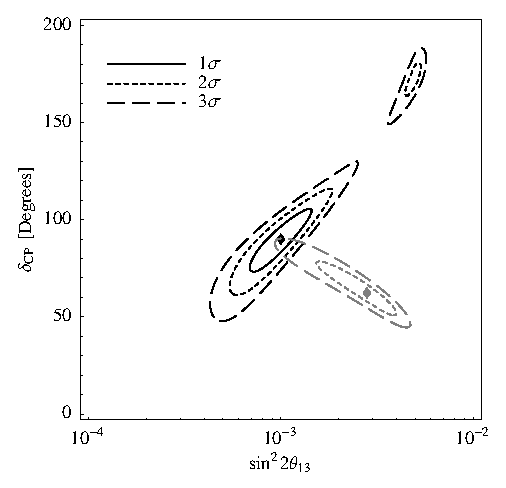
\includegraphics[width=7.5cm]{correntex}}
\end{center}

}

\index{All-parameter minimization}
The functions to perform the all-parameter minimization are {\tt ChiAll} and {\tt SingleChiAll}:
\begin{function}
\index{{\tt ChiAll}}
{\tt ChiAll}$(\{ \theta_{13}, \, \theta_{12}, \, \theta_{23}, \, \deltacp , \, \sdm , \, \ldm,  \, \hat{\rho_1}, \, \hdots , \, \hat{\rho_n} \})$ finds the local minimum close to the given starting point (list) for all initialized experiments. It returns the list  $\{ \chi^2, \, \theta_{13}, \, \theta_{12}, \, \theta_{23}, \, \deltacp , \, \sdm , \,  \ldm,  \, \hat{\rho_1}, \, \hdots , \hat{\rho_n} , \, N_{\mathrm{Iter}} \}$ with the minimum $\chi^2$-value, the actual position of the local minimum, and the number of iterations $N_{\mathrm{Iter}}$ used.
\end{function}
\begin{function}
\index{{\tt SingleChiAll}} 
{\tt SingleChiAll}$( \{ \theta_{13}, \, \theta_{12}, \, \theta_{23}, \, \deltacp , \, \sdm , \, \ldm, \,   \hat{\rho}_{N_{\mathrm{exp}}} \}, \, \, N_{\mathrm{exp}})$ finds the local minimum close to the given starting point (list) for the experiment $N_{\mathrm{exp}}$ only. It returns the list
 $\{ \chi^2, \, \theta_{13}, \, \theta_{12}, \, \theta_{23}, \, \deltacp , \, \sdm , \, \ldm, \, \hat{\rho}_{N_{\mathrm{exp}}} ,  \, N_{\mathrm{Iter}} \}$ with the minimum $\chi^2$-value, the actual position of the local minimum, and the number of iterations $N_{\mathrm{Iter}}$ used.
\end{function}
%
Both functions take the suspected position of the local minimum and return its true position. The application of  {\tt SingleChiAll} can be especially usefull for many different experiments evaluated simultaneously: It turns out to be useful to find the positions of the degeneracies for the individual experiments first, and then test all of these with the combination of all experiments in order not to miss a degenerate solution. The example on page~\pageref{ex:sgndeg} illustrates how to locate the $\mathrm{sgn}(\ldm)$-degeneracy and show the corresponding degenerate solution in the $\stheta$-$\deltacp$-plane together with the original solution.
In this case, the position of the degeneracy can be easily guessed to be at the best-fit parameter values but the $\ldm$ inverted. The minimizer then runs off the plane of the best-fit parameters into the local minimum. It is very important to take into account the position of the degeneracy off this plane, since the actual $\chi^2$ in the minimum is certainly lower than on the plane of the best-fit parameter values. Thus, the degeneracy may not even appear at the chosen confidence level on the plane, but it does appear at the true minimum. The two cuts\footnote{The discussed figure on page~\pageref{ex:sgndeg} is produced by  {\tt Chi} and thus only represents a cut through the fit manifold. For the projection including correlations, one may rather want to use {\tt ChiThetaDelta}.} through the fit manifold shown in the figure on page~\pageref{ex:sgndeg} therefore do not have the same oscillation parameter values (except from the ones shown in the figure). 

In practice, a number of tricks can be useful for the treatment of degenerate solutions:
\begin{description}
\item[Minimum $\boldsymbol{\chi^2}$ larger than threshold.] If a located degeneracy has a minimum $\chi^2$ larger than the corresponding confidence level threshold for the discussed quantity of interest, the degeneracy can be immediately ignored. This saves a lot of computation time.
\item[Locating degeneracies with more complicated topologies.] For more complicated topologies, such as for neutrino factories, it is often useful to use multi-step location procedures or analytical knowledge. For example, for a numerical procedure, one may first of all switch off the systematics and keep $\stheta$ or $\deltacp$ fixed, \ie, use {\tt SingleChiTheta} or {\tt SingleChiDelta}, where $\stheta$ or $\deltacp$ is fixed to the best-fit value. The result can then be used as a starting point for {\tt SingleChiAll} with the systematics switched on again. In addition to switching off the systematics, it can be useful to reduce the input errors during the first steps in order to make the minimizer not to run away too much from the true solution.
\item[Finding degeneracies with multiple experiments.] For multiple experiments, the degeneracies should be located for each of the individual experiments first. Then, all of the found degeneracies below the threshold can be tested for the combination of experiments.  
\end{description}
Finally, note that any degenerate solution below the confidence level threshold which can not be located makes the result appear better than it actually is. Thus, one should be careful with the determination of the degenerate solutions.

\chapter{Obtaining low-level information}

\bi
\item
 Obtaining rate vectors
\item
 Obtaining fluxes/cross sections etc.
\item
 ``Check''-functions
\ei

\example{The impact of systematics, correlations, and degeneracies}{
\label{ex:corrproj}
\index{Bar charts}
\index{Systematics on/off}

Here it is shown how one can successively include systematics, correlations,
and degeneracies at the example of the $\stheta$ sensitivity limit.
An important part of this example is how two switch the systematics off,
\ie, how to obtain the sensitivity limit from statistics only. Since
this example is very advanced, we only show the respective part of the code:
\begin{quote}
{\tt 
Here comes the code excerpt.
}
\end{quote}
The complete code can be found as ``example4.c'' with the software.

The returned lists of data then represent $\Delta \chi^2$ 
as function of the fit value of $\stheta$. The intersections of these
curves with the line $\Delta \chi^2 = 9$ give the $\stheta$ sensitivity
limits, where we do not include the $\mathrm{sgn}(\ldm)$- and $(\deltacp,\theta_{13})$-degeneracies in the sensitivity limit with
correlations only (green bar):
\begin{center}
\colorbox{white}{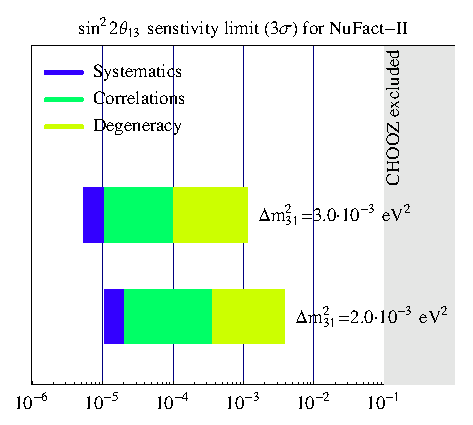
\includegraphics[width=7cm]{barsex}}

\end{center}
}

\chapter{Changing experiment parameters at running time}

\bi
\item
 Baseline, Target mass, Source power, running time
\item
 Matter density profile
\item
 Systematics
\item
 Threshold function, efficiencies etc.
\ei

%%%%%%%%%%%%%%%%%%%%%%%%%%%%%%%%%%%
% PART II: Experiment definition module
%%%%%%%%%%%%%%%%%%%%%%%%%%%%%%%%%%%

%%%%%%%%%%%%%%%%%%%%%%%%%%%%%%%%%%%
% PART II: Experiment definition module
%%%%%%%%%%%%%%%%%%%%%%%%%%%%%%%%%%%

\index{norm}{AEDL@\AEDL|(}
\part{The Abstract Experiment Definition Language -- AEDL}
\label{part:2}

\chapter{Getting started}

Here, the general concept of the AEDL is described and illustrated by an example. In addition, a short introduction to the syntax of the AEDL is given.

\section{General concept of the experiment simulation}

The goal of AEDL is to describe a large number of complex and very 
different experiments by a limited number of parameters. It allows a
representation of very different setups within one data structure, and thus implements universal rate and $\chi^2$ computation methods. For experiment simulations, usually a new piece of code is written and compiled
for each different experiment. In many cases, even parameter changes, such as
the number of bins, require the recompilation of the source code. 
However, such a technique soon reaches its limits when the simulated experiments are rather complex, or more than one type of experiment is studied simultaneously. Furthermore, it is very difficult to verify the correctness of the obtained results, since every time a new piece of code is added to 
deal with a new experiment type, new errors will be introduced.

Thus, a general and flexible experiment description language is needed.  
The description of a neutrino experiment can be split into three parts: Source, oscillation, and detection. The neutrino sources within \GLOBES\ 
are assumed to be stationary point sources, where each experiment has only 
one source. This restricts the classes of neutrino sources which can be studied with \GLOBES :
\begin{itemize}
\item
 Experiments using many point-like sources can only be approximated. One example are reactor experiments using many distant reactor blocks.
\item
 Geometrical effects of a source distribution, such as in the sun or the atmosphere, can not be described.
\item
 Sources with a physically significant time dependency  can not be studied, such as  supernov\ae. It is, however, possible
to study beams with bunch structure, since the time dependence of the
neutrino source is physically only important to suppress backgrounds. 
\end{itemize}

The description of the neutrino oscillation physics is, at least numerically, relatively simple. We use the {\em evolution operator method} (see, \eg, \Ref~\cite{Ohlsson:1999um})  to compute the neutrino oscillation probabilities and divide the matter density profile into layers of constant matter density. For each of these layers, the Hamiltonian in matter is diagonalized in order to propagate the neutrino transition amplitudes. Finally, the transition probability is obtained as the absolute square of the total neutrino transition amplitudes. Depending on the precision of the studied experiment, this approach turns out to be precise enough in Earth matter even if only a small number of matter density steps is used. Since we allow an uncertainty of the matter density profile, it is, in fact, in most cases sufficient to consider only one density step with the average matter density together with a matter density uncertainty~\cite{Ohlsson:2003ip}. Note that this approach may not be applicable to quickly varying extraterrestrial matter density profiles.

While it is comparatively simple to define a general neutrino source 
and to compute the oscillation physics, the general properties of a detector simulation are much more complicated. The basic assumption in building an abstract detector description is \emph{linearity}, \ie , that two neutrino events do not interfere with each other. Furthermore it is assumed that all information on the oscillation physics 
is given by the \emph{reconstructed} flavor and energy of a 
neutrino event. The term ``reconstructed'' implies that the well-defined energy of the incident neutrino, which can not be directly observed, translates via secondary particles and the detection properties into a distribution of possible energy values. This process is illustrated in \figu{distro} for the energy variable. 
%
\begin{figure}[ht]
\begin{center}
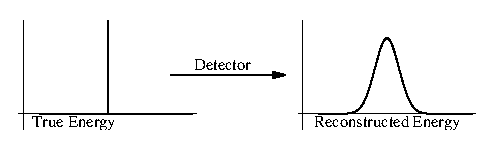
\includegraphics[width=0.6\textwidth]{mapping}
\end{center}
\mycaption{\label{fig:distro} A detector maps a true parameter value onto
a distribution of reconstructed parameter values. This is illustrated here for there energy.}
\end{figure}
% 
The same, in principle, applies to the nature of the neutrino flavor. However, in this case, only discrete values are applicable. Note that the reconstructed neutrino energy and the neutrino flavor are the only observables in \GLOBES .

This picture can also be formulated in a more mathematical way. Let us define $x$ as the true parameter value and $x'$ as the reconstructed parameter value. Similarly, $f(x)$ is the distribution of true parameters values and $p(x')$ is the distribution of reconstructed parameter values. Then the detector function  $D(x,x')$, which describes the mapping performed by the detector, is given by
\begin{eqnarray}
\label{equ:mapping}
p(x')&=&\int dx\, f(x)\cdot D(x,x')\,.
\end{eqnarray}
Obviously \equ{mapping} only describes the detector properly
if the linearity condition is fulfilled. Within this model, a detector
is completely specified by a set of $D(E,E')$ for the energy variable $E$,
and a set $D(F,F')$ for the flavor variable $F$. In general, $D(E,E',F)$ also depends on the incident neutrino flavor $F$, as well as $D(F,F',E)$ depends on the incident neutrino energy $E$. These sets of mapping functions usually are obtained from a 
full detector simulation and can be obtained by using as input 
distribution $f(x)$ a delta distribution $\delta(x-x_0)$.

\begin{figure}[t]
\begin{center}
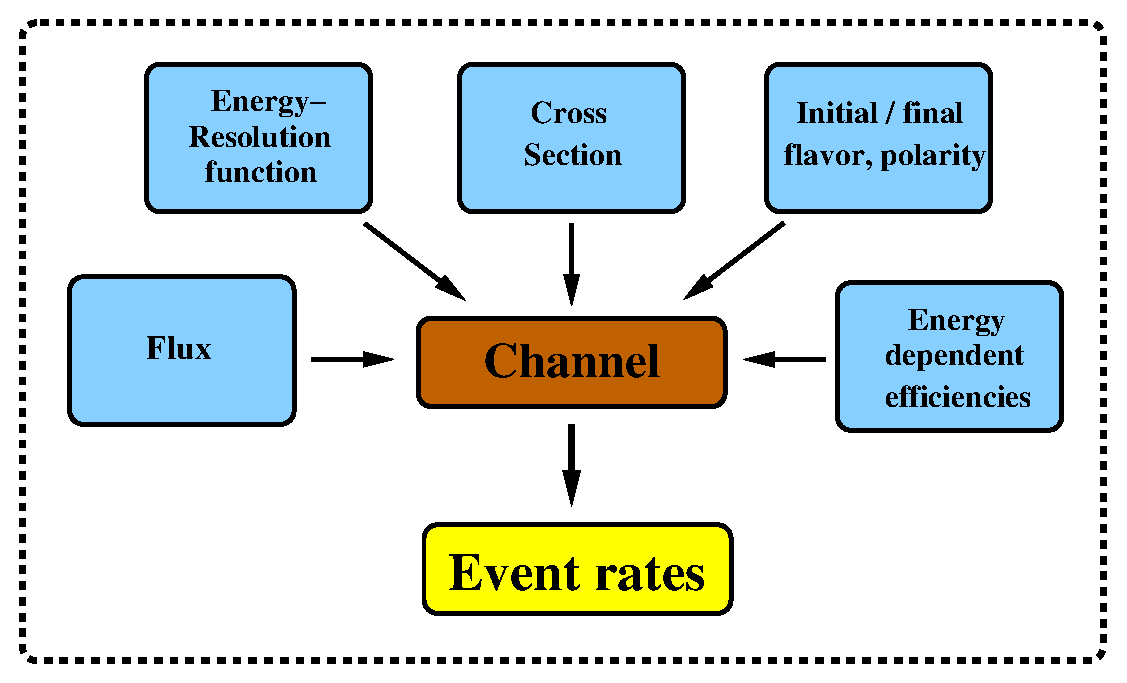
\includegraphics[width=13cm]{AEDL1}
\end{center}
\mycaption{\label{fig:channel} General concept of a ``channel''.}
\end{figure}

In order to implement an experiment definition including various
sources of systematical errors, we use several abstraction levels. 
The first level is the so-called ``channel'', \index{norm}{Channel}
 which is the link between 
the oscillation physics and the detection properties for a specfific oscillation pattern (\cf, \figu{channel}). A channel specifies the mapping of a specific neutrino flavor produced by the source onto a reconstructed neutrino flavor.
For example, a muon neutrino oscillates into an electron neutrino and subsequently interacts via quasi-elastic charged current scattering. The measured energy and direction of
the secondary electron in the detector then allows to reconstruct the neutrino energy. The connection from the source flux of the muon neutrino, via the  probability to appear as a electron neutrino, to its detection properties (such as cross sections and energy smearing) is encapsulated into the channel.

\begin{figure}[t]
\begin{center}
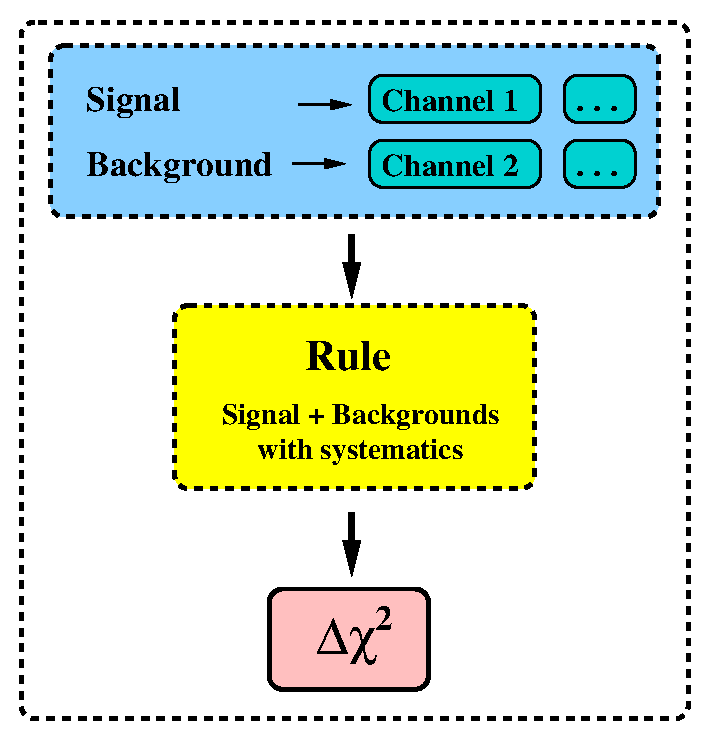
\includegraphics[width=8cm]{SignalBackground}
\end{center}
\mycaption{\label{fig:rule} General concept of a ``rule''.}
\end{figure}

\begin{figure}[t]
\begin{center}
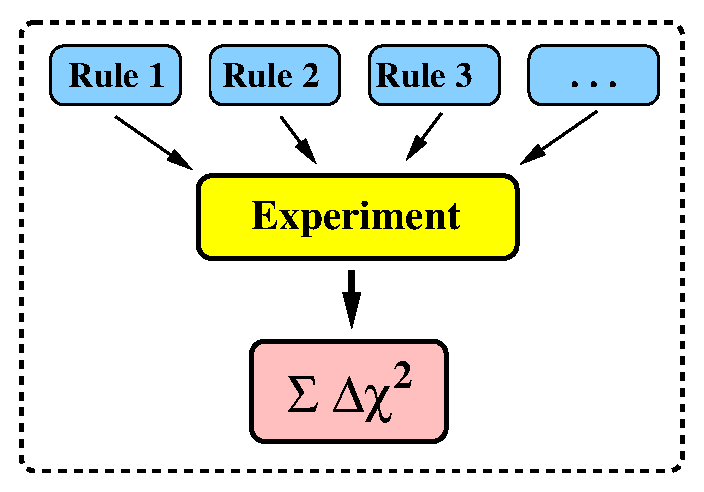
\includegraphics[width=9cm]{Rules}
\end{center}
\mycaption{\label{fig:experiment} General concept of an ``experiment''.}
\end{figure}

The channels are the building blocks for the so-called ``rules''.
\index{norm}{Rule} In general, a rule consists of one or more ``signal'' and ``background'' oscillation channels, which are normalized with efficiencies
(\cf, \figu{rule}). The event numbers from these channels are added {\em before} the $\Delta \chi^2$-value is calculated.\footnote{Note that
in this manual, the $\chi^2$ and $\Delta \chi^2$ are equal, since
for simulated data $\Delta \chi^2 = 0$ at the best-fit point. Thus, we
are using $\chi^2$ and $\Delta \chi^2$ as equal quantities.} In addition, each rule implements {\em independent} systematics, such as signal and background normalization errors. Eventually, each rule gives a $\Delta \chi^2$-value, and the total $\Delta \chi^2$ of one experiment is obtained by adding the $\Delta \chi^2$'s of all rules (\cf, \figu{experiment}). 
 An example for a rule could look like this: We want to detect electron
  neutrino appearance (``signal''), where the overall efficiency for 
  quasi-elastics electron neutrino events is $0.4$. There is a fraction of 
  $0.01$ of all neutral current events which are mis-identified as 
  quasi-elastic electron neutrino events (``background''). The neutral 
  current fraction is only known within $10\%$ (``background uncertainty'') 
  and there is
an energy scale uncertainty of $100\,\mathrm{MeV}$ (``energy calibration error'').
All this systematics is independent of the other rules.  Thus, a rule connects the event rates to the calculation of a $\Delta \chi^2$ which properly includes systematical errors. The resulting $\Delta \chi^2$ is then the starting point for the oscillation physics analysis. Note again that
\begin{itemize}
\item
 Within each rule, the event numbers are added.
\item
 Within each rule, the systematics is treated independently from the other rules.
\item
 For each rule, the $\Delta \chi^2$ is computed; the $\Delta \chi^2$'s from all rules are added.
\end{itemize}

Of course, an abstract experiment definition language can not simulate all possible types of experiments. As we have seen, there are several assumptions for source and detector. However, it turns out that \GLOBES\ can be applied to a large number of experiment types, such as conventional beams, superbeams, neutrino factories, $\beta$-Beams, and reactor experiments.

\section{A simple example for AEDL}

Experiments in \GLOBES\ are defined by the Abstract Experiment Definition Language (AEDL). The experiment definition is written into a text file using the AEDL syntax. Currently, a number of pre-defined experiment definition files are provided with \GLOBES , which have to be modified manually in order to define new experiments.  The application software then uses this text file to initialize the experiment, where other secondary files might be read for source fluxes, cross sections \etc . In this section, we show the definition of a very simple neutrino factory in AEDL, where we do not go into details. In the next chapter, we will discuss each of the individual steps in detail.

The first line of every experiment definition file has to be
\begin{quote}
{\tt !\%GLoBES}
\end{quote}
in order not to confuse it with some other file format.
In addition, \GLOBES\ 3.0 and higher requires the identification of the
minimum \GLOBES\ version the \AEDL\ file can be used with:
\begin{quote}
{\tt \$version="3.0.0"}
\end{quote}

%
First, we instruct \GLOBES\ to use the built-in source flux for a neutrino factory
originating from stored $\mu^+$'s. This is achieved by setting the {\tt @builtin} variable to $1$. Next, we specify the muon energy to be $50\,\mathrm{GeV}$ by the {\tt @parent\_energy} variable. We assume 
that there will be $5.33\cdot 10^{20}$ useful muon decays per year
and that this luminosity is available for $8$ years, \ie , a total number
of $ 4.264\cdot10^{21}$ muons is stored:
\begin{quote}
{\tt /* beam */}\\
{\tt nuflux(\#mu\_plus)<\\
\tb  @builtin = 1\\
\tb  @parent\_energy = 50.0\\
\tb  @stored\_muons = 5.33e+20\\
\tb  @time = 8.0\\
>}\\
\end{quote}
Note that we tell \GLOBES\ that we want to refer to this neutrino source later as as {\tt \#mu\_plus}. 
%
Let us now define a very simple detector with a target mass 
of $50\,\mathrm{kt}$ and $20$ energy bins between
$4\,\mathrm{GeV}$ and $50\,\mathrm{GeV}$: 
\begin{quote}
{\tt \$target\_mass = 50}\\
{\tt \$bins = 20}\\
{\tt \$emin = 4.0}\\
{\tt \$emax = 50.0}
\end{quote}
Then, we specify the file which contains the cross sections we want to 
use:
\begin{quote}
{\tt /* cross section */}\\
{\tt cross(\#CC)<}\\
{\tt \tb @cross\_file = "XCC.dat"}\\
{\tt >}
\end{quote}
The command {\tt cross} tells the parser that a cross section environment
begins. It has the name {\tt \#CC}, which can later be used to refer 
to this specific environment, and thus to the file {\tt XCC.dat}. Note that each name begins with a leading {\tt \#}.
%
Of course, the baseline and matter profile have to be specified, too, where
we use an arbitrary matter density profile here:
\begin{quote}
{\tt /* baseline */}\\
{\tt \$profiletype = 3}\\
{\tt \$densitytab = \{3.5\}}\\
{\tt \$lengthtab = \{3000.0\}}\\
\end{quote}
The curly brackets used for the definition of {\tt \$densitytab} and
{\tt \$lengthtab} refer to a list of numbers. Here, the lists contain only
one element each, because we only use one density layer: We specify a
baseline length of $3000 \, \mathrm{km}$ with a constant matter density of
$3.5 \, \mathrm{g/cm^3}$. 
%
As another ingredient, we have to define the energy resolution function:
\begin{quote}
{\tt /* energy resolution */}\\
{\tt energy(\#MINOS)<}\\
{\tt \tb @type = 1}\\
{\tt \tb @sigma\_e = \{0.15,0.0,0.0\}}\\
{\tt >}
\end{quote}
The {\tt energy} command starts the energy environment, which has the name 
{\tt \#MINOS} here. Out of several possibilities, it uses algorithm one,
the simplest and fastest one. The actual energy resolution is specified
by the energy resolution variable, which is a list of three elements. Each 
element is one parameter of the general resolution function as defined in 
\eq~\ref{eq:sigma_e}.
%
Now we have all pieces to be able to define the appearance and the corresponding disappearance channel of a neutrino factory: 
$\nu_e\rightarrow\nu_\mu$  and $\bar\nu_\mu\rightarrow\bar\nu_\mu$ 
($\mu^+$ stored).
\begin{quote}
{\tt /* channels */}\\
{\tt channel(\#appearance)<}\\
{\tt \tb @channel = \#mu\_plus: +: electron: muon: \#CC: \#MINOS}\\
{\tt >}\\
{\tt channel(\#disappearance)<}\\
{\tt \tb @channel = \#mu\_plus: -: muon: muon: \#CC: \#MINOS}\\
{\tt >}
\end{quote}
The first element is the name of the flux, which we have defined above. 
The second element ``$\pm$'' determines whether 
neutrinos or anti-neutrinos are taken from the flux table (two different polarities allowed). The third position defines the initial flavor,
and the forth position the final flavor, followed by the name of the cross
section and energy resolution function as defined before.
%
The last step is to encapsulate the channels into a rule:
\begin{quote}
{\tt /* rules */}\\
{\tt rule(\#rule1)<}\\
{\tt \tb @signal = 0.45 @ \#appearance}\\
{\tt \tb @signalerror = 0.025 : 0.0001}\\
{\tt \tb @background = 1.0e-05 @ \#disappearance}\\
%{\tt \tb @backgroundcenter = 1 : 0.0}\\
{\tt \tb @backgrounderror = 0.2 : 0.0001}\\
{\tt \tb @sys\_on\_function = "chiSpectrumTilt"}\\
{\tt \tb @sys\_off\_function = "chiNoSysSpectrum"}\\
{\tt \tb @energy\_window = 4.0 : 50.0}\\
{\tt >}
\end{quote}
The {\tt @signal} refers to the ``signal'' in our experiment. We use the
above defined channel named {\tt \#appearance} with a constant overall
efficiency of $0.45$ (in a more realistic simulation, one would introduce an
energy threshold function). The signal error variable has two components: 
The first one is the normalization error of the signal, here $2.5\%$. The second 
one refers to the energy calibration error of the signal, which is defined 
in \Sec~\ref{sec:energy}. The background variable
specifies the composition of the beam background. In this (simplified) case, we
use the fraction $1\cdot 10^{-5}$ of the channel named {\tt \#disappearance}, \ie , the muon neutrinos with a mis-identified charge. 
%The background center variable allows to rescale the total background contribution from all background components
%simultaneously. It is only useful if there is more than one background component, otherwise it is usually $1$. 
The background error variable is defined in the same way as the signal error variable, \ie , we have a $20\%$ background uncertainty and a very small energy calibration error. In addition, the systematics treatment is specified
in {\tt @sys\_on\_function} (for systematics switched on) and {\tt @sys\_off\_function} (for systematics switched off) -- see \Tab~\ref{tab:error_dim}. 

The experiment defined here represents a first simplified version of a neutrino factory experiment. It still lacks the correct energy dependence of the efficiencies, the antineutrino disappearance channel, and the channels and rules for the symmetric operation with $\mu^-$ stored. However, it may serve as a simple, introductory example. In the next chapter, we will demonstrate that AEDL is much more powerful than illustrated here.


%%%%%%%%%%%%%%%%%%%%%%%%%%%%%%%%%%%%%%%%%%%%%%%%%%%%%%%%%%%%%%%%%%%%%%%%
\section{Introduction to the syntax of AEDL}
\label{sec:syntax}

We now give a short introduction to the syntax of AEDL.
 The first eight characters have to be {\tt \%!GLoBES}
in order to avoid parsing megabytes of chunk
 and producing thousands of error messages.  In addition, the minimum
\GLOBES\ version that the \AEDL\ file is supposed to run with has to be
defined by a {\tt \$version} statement, such as
{\tt \$version="3.0.0"}.
\index{aedl}{version@{\tt \$version}}
%
Comments can be used in the same way as in C:
\begin{quote}
{\tt /* This starts a comment\\
 and here the comment ends */ \\
// Another comment
}
\end{quote}
There are pre-defined variables which all start with {\tt \$}. Their range
is also checked. For example,  {\tt 
\$bins} can be only between $0$ and $500$.\footnote{The upper limit is 
only there for safety reasons, the memory is allocated dynamically.} If one uses a {\tt float} quantity where  an {\tt int} is expected, the {\tt float} will be converted to an {\tt int} in the same way as in C.  For example, we have scalar variables
\begin{quote}
{\tt
\$bins = 10\\
\$baseline = 1200.0
}
\end{quote}
and simple lists
\begin{quote}
{\tt
\$densitytab=\{1.0,2.2343,3.3432\} 
}
\end{quote}
%
Since there are often groups of data which we want to refer to later,
environments can be used. This is illustrated 
with the channel definition part:
\begin{quote}
{\tt channel(\#ch1)<\\
\tb  $\ldots$\\
>
}
\end{quote}
The first part is the type of environment, which is {\tt channel} here. 
There are the following types of environments in AEDL:
\begin{quote}
{\tt nuflux\\
cross\\
channel\\
energy\\
rule
}
\end{quote}
Besides the environment type, there is a user-defined name 
beginning with {\tt \#}
in the above example: {\tt \#ch1}. It can be used later to refer to the 
channel defined in {\tt <$\ldots$>}. Those names are so-called 
``automatic variables'' and have to start with {\tt \#}. Note that these names have to be unique and can only be refered to after their definition.
However, similar to C, one can give a declaration without definition before:
\begin{quote}
{\tt    channel(\#ch2)<>}
\end{quote}
Now one can refer to the name {\tt \#ch2}, while the actual channel definition comes later. The internal representation of this automatic
variable is a number, which obtains its value from a counter for each type of environment. For example, for {\tt channel} the counter is {\tt numofchannels}. The counter keeps track of how many different names 
there are for one type of environment, which means that it counts the number of channels, rules, energy resolution functions, \etc . Thus, the automatic
variables are numbered in the order of their definition, and the number
can later be used to refer to them in the C code (from $0$ to {\tt numof...}$-1$). In order to facilitate the the mapping from names in AEDL to indices
in C there are two functions \GLB{NameToValue} and \GLB{ValueToName} which
make this transition (see \Sec~\ref{sec:aedl_names}, 
page~\pageref{sec:aedl_names}).


Within each environment type, there are several 
variables beginning with {\tt @}, which can only be used within the 
appropriate type of environment. In many cases, 
they have a special syntax, such as {\tt @channel}.

\index{aedl}{NEXT@{\tt \#NEXT\#}}
If you want to have several experiments in one file, separate the different
 experiments by 
\begin{quote}
{\tt    \#NEXT\#}
\end{quote}
This command resets the counters for channels, rules, fluxes, cross section 
and energy resolution environments. All variables have their scope limited 
by either {\tt \%!GLoBES, \#NEXT\#} or {\tt EOF}.  This allows 
a consistent treatment of various experiments in one file.

\index{aedl}{include@{\tt include}}
As another feature of AEDL one, can use include files with the {\tt include} command. Includes can be nested up to {\tt MAX\_INCLUSION\_DEPTH}, which is currently set to $10$. Error reporting works 
 for nested includes, too. The included file is not required to begin 
 with {\tt \%!GLoBES} to facilitate cut and paste:
\begin{quote}
{\tt include "./file\_1"}
\end{quote}
With this include mechanism, one can use constructions such as 
\begin{quote}
{\tt    include  "Exp1.glb"\\
        \#NEXT\#\\
        include   "Exp2.glb"
}
\end{quote}
in order to initialize a combined analysis of the experiments defined in the files {\tt Exp1.glb} and {\tt Exp2.glb}. Note that one has 
to use quotation marks for filenames in \AEDL.\index{norm}{File names}
Even if one uses the
automatic variable {\tt \#CC} in both experiments, 
but the cross section data are different (for example, because of different target nuclei), the correct 
cross section data will be applied to each of the experiments. 
Note that, alternatively, one can 
also load both files successively by two separate calls of 
\GLB{InitExperiment}. 

Furthermore, one can define constants such as
\begin{quote}
{\tt
Pi = 3.14159
}
\end{quote}
These constants can not only be defined within one \AEDL\ file, but also
by the calling C program, which allows to use a simple but powerful variable
substitution mechanism as described in~\Sec~\ref{sec:aedlparams}.
\index{norm}{AEDL@\AEDL!external parameters}

In addition, some simple algebraic manipulations are possible, such as
\begin{quote}
{\tt
Pi+1\\
\verb+Pi^2+\\
sin(Pi/2)
}
\end{quote}
The following mathematical functions from {\tt <math.h>} are available: 
{\tt sin}, {\tt cos}, {\tt tan}, {\tt asin}, {\tt acos}, {\tt atan}, 
{\tt log}, {\tt log10}, {\tt exp}, {\tt sqrt}.
\index{aedl}{sin@{\tt sin}}%
\index{aedl}{cos@{\tt cos}}%
\index{aedl}{tan@{\tt tan}}%
\index{aedl}{asin@{\tt asin}}%
\index{aedl}{acos@{\tt acos}}%
\index{aedl}{atan@{\tt atan}}%
\index{aedl}{log@{\tt log}}%
\index{aedl}{log10@{\tt log10}}%
\index{aedl}{exp@{\tt exp}}%
\index{aedl}{sqrt@{\tt sqrt}}%
% 
These functions can be used everywhere, where
otherwise only a scalar number would appear. However, they can not be
applied to lists, \ie, expressions like {\tt sin(\{1,2,3\})} will not work. 

Finally, note that a line feed character \verb+\n+ is necessary at
 the end of the input -- alternatively you can put a comment at the end.

\section{More advanced AEDL features}
\label{sec:advaedl}

In \GLOBES\ 3.0 and higher, a number of new features can be used. The
features in this section are slighlty more advanced and can be skipped in a first reading of
the manual. The
most important one are lists as variables in \AEDL . They start with {\tt \%}, such as
\begin{quote}
{\tt
\%effs = \{ 0.2, 0.4, 0.6, 0.8, 1.0, 1.0, 1.0 \}
}
\end{quote}
Functions can be threaded over lists, \ie, they will be applied to each element
of list, and return a list. Note that the original list will be destroyed by this
process. Therefore, it is necessary to create a copy of your list if you want to
use the original and the threading result. For that purpose, the {\tt copy}
funcion is provided:
\begin{quote}
{\tt
 listb = copy(lista) \\
 listb := lista // Alternative method 
}
\end{quote}
\index{aedl}{copy@{\tt copy}}
You will also need to use {\tt copy} when you assign a list to an experiment structure (see below).

Two helper functions {\tt bincenter()} 
\index{aedl}{bincenter@{\tt bincenter}} and {\tt samplingbincenter} \index{aedl}{samplingbincenter@{\tt samplingbincenter}} return lists with the central energies of the bins or sampling points, respectively. For example,
\begin{quote}
{\tt
 \%bc=bincenter() 
}
\end{quote}
A very useful new features is an interpolation function which can directly interpolate a number of
points and evaluate them at a different set of places. For example,
\begin{quote}
{\tt
 \%energ = \{ 4.0,20.0,50.0 \} \\
 \%effs = \{ 0.0,1.0,1.0 \} \\
 \%ires = interpolation(\%energ,\%effs,1,\%bc) 
}
\end{quote}
\index{aedl}{interpolation@{\tt interpolation}}
interpolates the points with x-values {\tt \%energ} and y-values {\tt \%effs} with the interpolation order one (linear interpolation, third parameter) and evaluates the interpolation result at the bin centers obtained above, \ie, it returns a list of the y-values at the places specified by the last parameter. The only allowed interpolation orders are ``1'' (linear) and ``2'' (cubic splines). This example creates
a neutrino factory energy threshold function linearly climbing from 0 to 1 between 4~GeV and 20~GeV. It can be directly used in a channel definition, \eg, 
\begin{quote}
{\tt
 channel(\#nu\_mu\_appearance)< \\
\hspace*{0.5cm}	@channel = \#mu\_plus: +: electron: muon: \#CC: \#MINOS\ \\
\hspace*{0.5cm}	@post\_smearing\_efficiencies = copy(\%ires) \\
>
}
\end{quote}


To simplify debugging of lists and numbers, \GLOBES\ now supports output directly
from \AEDL\ files:
\begin{quote}
{\tt 
 R = 1.15 \\
 echo(R) // Print without line feed \\
 line(2) // Two line feeds \\
 echon(ires) // Print with line feed 
}
\end{quote}
\index{aedl}{echo@{\tt echo}}
\index{aedl}{echon@{\tt echon}}
\index{aedl}{line@{\tt line}}



%%%%%%%%%%%%%%%%%%%%%%%%%%%%%%%%%%%%%%%%%%%%%%%%%%%%%%%%%%%%%%%%%%%%%%%
\chapter{Experiment definition with AEDL}

In this chapter, we give a detailed description of the \AEDL\ features. We also show the underlying mathematical concepts where applicable. We do not exactly follow the separation of source, oscillation, and detection properties, since most issues more or less involve the detection. Instead,
we illustrate many of the features of the \GLOBES\ simulation successively
in the logical order of their definition, and demonstrate how they translate into \AEDL .

%%%%%%%%%%%%%%%%%%%%%%%%%%%%%%%%%%%%%%%%%%%%%%%%%%%%%%%%%%%%%%%%%%%%%%%%
\section{Source properties and integrated luminosity}
\label{sec:source}

As we have disussed before, \GLOBES\ can only deal with point sources. Thus,  it is not possible to study effects of the finite size of the neutrino production region, such as in the sun or in reactor experiments with many
neutrino sources (\eg, KamLAND). Therefore, a neutrino source in \GLOBES\ can, in general, be characterized by the flux spectrum for each neutrino flavor, the CP sign (neutrinos or antineutrinos), and the total luminosity
of the source.

Before we come to the definition of the source properties, let us discuss
the total integrated luminosity of the experiment. In \GLOBES , the total number of events is in general proportional to the product of
\begin{equation}
\mathrm{Fid.~detector~mass}\,\left[\mathrm{kt/t}\right]\times 
\mathrm{Running~time} \,\left[\mathrm{yr}\right]\times\left\{ \begin{array}{c}
\mathrm{Source~power}\,\left[\mathrm{MW/GW}\right]\\
\mathrm{Useful~parent~decays}\,\left[\mathrm{yr}^{-1}\right]
\end{array}\right.\,.
\end{equation}
Thus, the source power corresponds to either the amount of energy produced per time frame in the target (such as for nuclear reactors or sources based on pion decay), or the useful parent particle decays per time frame (neutrino factories, beta beams). In addition, the definition of the source power makes only sense together with the flux normalization, the running time, and the fiducial detector mass in order to define the total integrated luminosity. Therefore, one can, in principle, use arbitrary units for these components as long as their product gives the wanted neutrino flux. However, it is
recommended to use normalizations such that the source power units are $\mathrm{MW}$ for a proton-based beam, and $\mathrm{GW}_\mathrm{thermal}$ for a reactor experiment. Correspondingly, the detector mass units should be kilotons for a proton-based beam, and tons for a reactor experiment. In any case it is a good
idea to document the choices made by the user by corresponding comments
in \AEDL. For more details on the luminosity implementation, see appendix on page~\pageref{app:flux}.

\index{aedl}{target mass@{\tt \$target\_mass}}
The quantity which can be used to scale the overall integrated luminosity of an experiment, is the fiducial detector mass. For example,
\begin{quote}
{\tt \$target\_mass = 50.0 }
\end{quote}
defines a $50 \, \mathrm{kt}$ detector for a neutrino factory.

\index{aedl}{nuflux@{\tt nuflux}!time@{\tt "@time}}
There are two principal ways to initialize a neutrino flux: 
Either one can use 
a built-in source, or one can provide a file. In both cases,
a flux is defined by the environment {\tt nuflux}, such as
\index{aedl}{nuflux@{\tt nuflux}}
\begin{quote}
  {\tt nuflux(\#name)<\\
\tb $\ldots$\\
\tb @time = 8.0 \\
>}
\end{quote}
with a running time of $8$ years. Note that the running time is used within
the {\tt nuflux} environment. This feature can be used to load the neutrino
and antineutrino fluxes in an accelerator experiment separately, in order
to combine them with different running times in the respective operation modes.
The name of the flux {\tt \#name} will later be referred to in the channel definitions. Note that \GLOBES\ versions older than 3.0 use the still supported {\tt flux} environment, which is different from {\tt nuflux} by an undocumented normalization factor 5.2 for user-defined fluxes. This difference is explained in the appendix on page~\pageref{app:flux}.

\index{aedl}{nuflux@{\tt nuflux}}

\begin{table}[t]
\begin{center}
\begin{tabular}{|cllc|}
\hline
{\tt @builtin} & Description & Parameters & Min. version \\
\hline
1 & Neutrino factory $\mu^+$ decay & {\tt @parent\_energy} [GeV], & 2.0 \\
& & {\tt @stored\_muons} &  \\
2 & Neutrino factory $\mu^-$ decay & {\tt @parent\_energy} [GeV], & 2.0 \\
& & {\tt @stored\_muons} &  \\
3 & Beta beam, inv. beta decay & {\tt @end\_point} [GeV], & 3.0 \\
& & {\tt @stored\_ions}, &  \\
& & {\tt @gamma} & \\
4 & Beta beam, beta decay & {\tt @end\_point} [GeV], & 3.0 \\
& & {\tt @stored\_ions}, &  \\
& & {\tt @gamma} & \\
\hline
\end{tabular}
\end{center}
\mycaption{\label{tab:binfluxes} Built-in fluxes currently supported by \GLOBES . For details on
the beta beams, see \Ref~\cite{Huber:2005jk}. MR ABOUT BETA BEAMS: DOES THIS REALLY WORK FOR ALL ISOTOPES? IS THE DIFFERENCE BETWEEN 3 AND 4 CORRECTLY DESCRIBED? WHY IS THERE A NORMALIZATION FACTOR 50.9 IN THE FILES?}
\end{table}

For a built-in neutrino source, one has to specify which
built-in spectrum should be used, as well as its parameters. The software
will then automatically calculate the neutrino spectrum. Note that in this
case, there is no degree of freedom in the choice of the source units.
The currently available fluxes are described in \Tab~\ref{tab:binfluxes}.
For example, two built-in neutrino factory fluxes are available: $\mu^+$-decay ({\tt @builtin = 1}) and $\mu^-$-decay ({\tt @builtin = 2}). In these cases, the muon energy (enery of the parent particle) has to be specified together with the number of useful decays  per year. Thus, an example to set up a neutrino factory flux is 
\index{aedl}{nuflux@{\tt nuflux}!builtin@{\tt "@builtin}}
\index{aedl}{nuflux@{\tt nuflux}!parent energy@{\tt "@parent\_energy}}
\index{aedl}{nuflux@{\tt nuflux}!stored muons@{\tt "@stored\_muons}}
\index{aedl}{nuflux@{\tt nuflux}!end point@{\tt "@end\_point}}
\index{aedl}{nuflux@{\tt nuflux}!stored ions@{\tt "@stored\_ions}}
\index{aedl}{nuflux@{\tt nuflux}!gamma@{\tt "@gamma}}
\begin{quote}
{\tt nuflux(\#mu\_plus)<\\
\tb  @builtin = 1\\
\tb  @parent\_energy = 50.0\\
\tb  @stored\_muons = 5.33e+20\\
\tb  @time = 8.0\\
>}
\end{quote}
MR: SOME MORE ELABORATION AND AN EXAMPLE FOR THE BETA BEAMS MAY BE APPROPRIATE HERE [WW].
%
\index{aedl}{nuflux@{\tt nuflux}!power@{\tt "@power}}
\index{aedl}{nuflux@{\tt nuflux}!norm@{\tt "@norm}}
\index{aedl}{nuflux@{\tt nuflux}!flux file@{\tt "@flux\_file}}
For a user-defined flux, one has to specify the file name:
\begin{quote}
{\tt nuflux(\#user)<}\\
{\tt \tb @flux\_file = "user\_file\_1.dat"\\
\tb @time = 2.0\\
\tb @power = 4.0\\
\tb @norm = 1e+8}\\
{\tt >}
\end{quote}
In this case, the {\tt @norm} variable is an overall normalization which defines a conversion factor from the fluxes in the file to the units in \GLOBES . In general, there are many ways to give the source power of a 
neutrino source, such as neutrinos per proton on target per area per time frame. Right now, each flux has its own normalization factor, which is
not always straightfoward to calculate. Often, one has to take into account
many things, such as the number of target particles per unit mass. 
In addition, the fluxes will be rescaled by $1/L^2$, which means that the
normalization must contain a factor $L_0^2$. Here $L_0$ is the distance from the source for which the flux is given to the actual neutrino production region. At the end, it is left to the user to ensure that the 
numbers in the flux file give, after the multiplication with {\tt @norm}, 
the proper numbers of produced neutrinos corresponding to the chosen target power {\tt @power}. Usually this adjustment of {\tt @norm} is performed by comparison with known energy spectra for a specific experiment.
For more details on the flux definition, see page~\pageref{app:flux} in the appendix.

\index{aedl}{nuflux@{\tt nuflux}!flux file@{\tt "@flux\_file}}\index{norm}{Flux!file}
The software assumes that the given flux file has seven columns and
501 lines with equidistant energies. The format is:
\begin{quotation}
$ E\quad
\Phi_{\nu_e}\quad
\Phi_{\nu_\mu}\quad
\Phi_{\nu_\tau}\quad
\Phi_{\bar\nu_e}\quad
\Phi_{\bar\nu_\mu}\quad
\Phi_{\bar\nu_\tau}$
\end{quotation}
In order to access fluxes at arbitrary energies, linear interpolation 
is used by \GLOBES. In general, it is advisable to provide the flux
between {\tt \$sampling\_min} and {\tt \$sampling\_max} (\cf, \Sec~\ref{sec:energy}),
since this is the energy range considered in the simulation. However,
if part of this interval is omitted in the flux file, zero will be
used there. If some neutrino flavours are not used in the simulation,
the corresponding columns in the flux file have to be filled nevertheless,
\eg\ with zeros. 

The flux files accept one-line comments, which start
with {\tt \#} and end with the linefeed character `\verb+\n+', they are
not counted as a line and their content is discarded. These comments
are useful to provide meta information about the fluxes such as units
or the origin of the information. This is also the default method
to point the user to the references that should be cited when using
a particular flux file.\index{norm}{Flux!file!comments in}
\index{norm}{Referencing!flux data}

%%%%%%%%%%%%%%%%%%%%%%%%%%%%%%%%%%%%%%%%%%%%%%%%%%%%%%%%%%%%%%%%%%%%%
\section{Baseline and matter density profile}

Besides the energy and the involved flavors, the neutrino oscillation
physics depends on the baseline and the matter density profile.
All neutrino oscillation parameters are defined at running time.

\index{aedl}{baseline@{\tt \$baseline}}
The baseline\index{norm}{Baseline} is given by
\begin{quote}
{\tt \$baseline = 3000.0 }
\end{quote}
Note that baseline lengths are always assumed to be in
kilometers.

\begin{table}[t!]
\begin{tabular}{|clp{7cm}|}
\hline
{\tt \$profiletype} & Additional variables & Description \\ 
\hline
$1$ & {\tt \$baseline} & Average density (constant) \\
$2$ & {\tt \$baseline}, {\tt \$densitysteps} & PREM profile with given number of equidistant steps \\
$3$ & {\tt \$lengthtab},  {\tt \$densitytab} & Arbitrary profile (table of layer thicknesses, table of densities) \\
\hline
\end{tabular}
\mycaption{\label{tab:profiletypes} Different matter density profiles which can be used with \GLOBES .}
\end{table}

\index{aedl}{profiletype@{\tt \$profiletype}}
\index{aedl}{densitysteps@{\tt \$densitysteps}}
\index{aedl}{lengthtab@{\tt \$lengthtab}}
\index{aedl}{densitytab@{\tt \$densitytab}}

Furthermore, the matter density profile along the baseline
has to be specified. The simplest profile is a constant matter density equal to the average matter density from the PREM~\cite{Stacey} onion shell model of the earth:\index{norm}{PREM| \see{Matter density}}
\index{norm}{Matter density!of the earth}
\begin{quote}
{\tt \$profiletype=1 }
\end{quote}
%
If you are using this option please cite reference~\cite{Stacey}\index{norm}{Referencing!matter profile data}.

For a better approximation of the realistic earth matter density profile, one can use an arbitrary number of equidistant steps of the PREM profile:
\begin{quote}
{\tt \$profiletype=2 } \\
{\tt \$densitysteps=20 }
\end{quote}
Note that the value of {\tt \$densitysteps} is time-critical, since the
computation time of oscillation probabilities is directly 
proportional to the number of layers.
%
As a  third possibility, one can specify the matter density profile 
manually with a list of thicknesses and densities of the matter density layers. This example uses two density steps with two different densities:
\begin{quote}
{\tt \$profiletype=3 } \\
{\tt \$densitytab=\{2.8, 3.5\}}\\
{\tt \$lengthtab=\{1000.0, 2000.0\}}
\end{quote}
It is important that both lists have the same length and that the  thicknesses given in  {\tt \$lengthtab} add up to the length of
the baseline, which does not have to be explicitely specified anymore. In addition, matter densities are always given in $g/cm^3$.
%
This approach can also be used for a constant matter density profile with
a specific matter density:
\begin{quote}
{\tt \$profiletype=3 } \\
{\tt \$densitytab=\{3.5\}}\\
{\tt \$lengthtab=\{3000.0\}}
\end{quote}
The possible options for matter density profiles are summarized in \Tab~\ref{tab:profiletypes}.

%%%%%%%%%%%%%%%%%%%%%%%%%%%%%%%%%%%%%%%%%%%%%%%%%%%%%%%%%%%%%%%%%%%%%%%%%%%%%

\section{Cross sections}
\label{sec:cross_section}

Cross sections\index{norm}{Cross section} will later be used as part of the 
channel definition (see \Sec~\ref{sec:channel}). Similar to the source 
fluxes, they are provided by the user as a data file:
\index{aedl}{cross@{\tt cross}}
\index{aedl}{cross@{\tt cross}!cross file@{\tt  "@cross\_file}}
\begin{quote}
{\tt cross(\#name)<}\\
{\tt \tb @cross\_file ="user\_file\_1.dat"}\\
{\tt >}
\end{quote}  
This cross section can later be refered to by {\tt \#name}.

Cross sections in \GLOBES\ are given as total cross section divided by energy:
\begin{equation}
\hat\sigma(E)=\sigma(E)/E\,\left[ 10^{-38}\,
\frac{\mathrm{cm}^2}{\mathrm{GeV}} \right]
\end{equation}
The software assumes that the cross section files are text files with 
seven columns and $1001$ lines of the form
\index{norm}{Cross section!file}
\index{aedl}{cross@{\tt cross}!cross file@{\tt  "@cross\_file}}
\begin{quotation}
$\mathrm{log}_{10} E\quad
\hat\sigma_{\nu_e}\quad
\hat\sigma_{\nu_\mu}\quad
\hat\sigma_{\nu_\tau}\quad
\hat\sigma_{\bar\nu_e}\quad
\hat\sigma_{\bar\nu_\mu}\quad
\hat\sigma_{\bar\nu_\tau}$
\end{quotation}
Here the logarithms of the energy values have to be equidistant. For 
arbitrary energies, linear interpolation is used. If the energy leaves the
range of values given in the file, $0.0$ will be assumed. In general, it is advisable to provide the cross sections in the range between {\tt \$sampling\_min} and {\tt \$sampling\_max} (\cf, \Sec~\ref{sec:energy}).
Cross sections for unused neutrino flavours have to be filled with zeros, and
can not just be omitted.

Like the flux files, the cross section files 
accept one-line comments, which start
with {\tt \#} and end with the linefeed character `\verb+\n+'; they are
not counted as a line and their content is discarded. These comments
are useful to provide meta information about the cross sections like units
or the origin of the information. This is also the default method
to point the user to the references he/she should cite when using
a particular cross section file.\index{norm}{Cross section!file!comments in}
\index{norm}{Referencing!cross section data}

\section{Oscillation channels}
\label{sec:channel}

\index{aedl}{channel@{\tt channel}|(}
Channels\index{norm}{Channel} in \GLOBES\ represent an intermediate level 
between the pure oscillation physics given by the oscillation probability
$P_{\alpha\beta}$, and the final event rates composed of signal and 
background. A channel describes the path from one
initial neutrino flavor in the source to the event rates in the detector for one specific interaction type (IT) and final flavor.  
Therefore, a channel contains the description of the 
initial neutrino flavor, its CP eigenvalue 
(neutrino or antineutrino)\footnote{Currently, \GLOBES\ does not support lepton
number violating transitions, \ie\ no transitions from neutrino to 
antineutrino (or vice versa) are considered.}, 
the detected neutrino flavor, the interaction cross sections for the chosen interaction type, and the energy resolution function of the detector.

Before we come to the definition of channels in AEDL, we introduce the general concept for the calculation of event rates. The first step is to
compute the number of events for each IT in the detector for each 
initial and final neutrino flavor and energy bin. The second step is to include the detector effects coming from the insufficient knowledge in the event reconstruction.
The combination of these two steps leads to the differential event rate spectrum for each initial and final flavor and IT as seen by the detector, which we call the ``channel''. In this section, we focus on the
 first step, \ie , we discuss the definition of the energy resolution function in the next section, since this is a rather comprehensive issue.

The differential event rate for each channel is given by
%%%%%%%%%%%%%%%%%%%%%%%%%%%%%%%%%%%
\begin{eqnarray}
\label{eq:master_event}
\frac{dn_{\beta}^{\text{IT}}}{dE'}=&&N\,\int\limits_0^\infty \int\limits_0^\infty dE\,d\hat{E}\quad
\underbrace{\Phi_{\alpha} (E)}_{\mathrm{Production}} \times \nonumber\\
&&\underbrace{\frac{1}{L^2} P_{(\alpha\rightarrow\beta)}(E,L,\rho;\theta_{12},
\theta_{13},\theta_{23},
\Delta m^2_{31},\Delta m^2_{21},\deltacp)}_{\mathrm{Propagation}}
\times \nonumber \\ &&\underbrace{\sigma^{\text{IT}}_f(E)
k_f^{\text{IT}}(E-\hat{E})}_{\mathrm{Interaction}} \times \nonumber \\
&&\underbrace{ T_f(\hat{E}) V_f(\hat{E}-E')}_{\mathrm{Detection}}\,,
\end{eqnarray}
%%%%%%%%%%%%%%%%%%%%%%%%%%%%%%%%%%%
where $\alpha$ is the initial flavor of the neutrino, 
$\beta$ is the final flavor, $\Phi_{\alpha} (E)$ is the flux of the 
initial flavor at the
source, $L$ is the baseline length, $N$ is a normalization factor, and 
$\rho$ is the matter density. The energies in this formula are given as follows:
\begin{itemize}
\item
 $E$ is the incident neutrino energy, \ie, the actual energy of the 
incoming neutrino (which is not directly accessible to the experiment)
\item
 $\hat{E}$ is the energy of the secondary particle
\item
 $E'$ is the reconstructed neutrino energy, \ie, the measured
neutrino energy as obtained from the experiment
\end{itemize}
The interaction term is composed of 
two factors, which are the total cross section 
$\sigma^{\text{IT}}_\beta(E)$ for the flavor $f$ and
the interaction type IT, and the energy distribution of the 
secondary particle $k_\beta^{\text{IT}}(E-\hat{E})$.
The detector properties are 
modeled by the threshold function $T_\beta(\hat{E})$, coming from the the 
limited resolution or the cuts in the analysis, and the energy resolution 
function $V_\beta(\hat{E}-E')$ of the secondary particle. 

Since it is computationally very expensive to solve this double integral
numerically, we split up the two integrations. The integral over $\hat{E}$
depends only on the terms containing $\hat{E}$, i.e., on $k_\beta^{\text{IT}}(E-\hat{E})$,
$ T_\beta(\hat{E})$, and $V_\beta(\hat{E}-E')$. These terms do not depend
on the oscillation parameters, so they will not vary during the fit,
and the $\hat{E}$ integral can be pre-computed in the initialization phase.
We define:
\begin{eqnarray}
\label{eq:e_res} 
R_\beta^{\text{IT}}(E,E')\,\epsilon_\beta^{\text{IT}}(E')
 \equiv
\int\limits_0^\infty d\hat{E} \quad T_\beta(\hat{E})\,k_\beta^{\text{IT}}(E-\hat{E})
\,V_\beta(\hat{E}-E')\,. 
\end{eqnarray}
Thus, $R_\beta^{\text{IT}}(E,E')$ describes the energy response of 
the detector, \ie , a neutrino with a (true) energy $E$ is reconstructed
with an energy between $E'$ and $E'+dE'$ with a probability
$R_\beta^{\text{IT}}(E,E') dE'$. The function $R(E,E')$ is often called ``energy resolution function''. Actually, its internal representation
in the software is a smearing matrix\index{norm}{Energy!resolution}\index{norm}{Smear matrix}. The function $\epsilon_\beta^{\text{IT}}(E')$ will later be refered to as ``post-smearing efficiencies'', since it will allow us to define cuts and threshold functions {\em after} the smearing is performed, \ie, as function of $E'$. The detailed definition and initialization of the energy resolution function is described in \Sec~\ref{sec:energy}.

Eventually, we can write down the number of events per bin $i$ \index{norm}{Bin} and channel $c$ as
\begin{equation}
\label{eq:channel}
n_i^c=\int_{E_i-\Delta E_i/2}^{E_i+\Delta E_i/2} dE' \quad
\frac{dn_{\beta}^{\text{IT}}}{dE'} (E') \,
\end{equation}
where $\Delta E_i$ is the bin size of the $i$th energy bin.
This means that one has to solve the integral
\begin{eqnarray}
\label{eq:events_bin}
n_i^c=N/L^2\,\int_{E_i-\Delta E_i/2}^{E_i+\Delta E_i/2} dE' 
\quad \int\limits_0^\infty dE \,\, \Phi^c(E)\,
P^c(E)\,
\sigma^c(E)\,
R^c(E,E')\,
\epsilon^c(E')\,.
\end{eqnarray} 
Note that the events are binned according to their \emph{reconstructed} energy.

A simple channel definition in \GLOBES\ consists of the flux,
the CP-sign of the initial state, the initial flavor, the final flavor,
the cross sections, and the energy resolution function. In order to refer to
the fluxes, cross sections, and energy resolution functions, they have to be 
defined first with their {\tt \#name} in the respective environments. 
A simple definition of a channel\index{aedl}{channel@{\tt channel}} is
\begin{quote}
{\tt channel(\#channel\_1)<\\
\tb @channel = \#flux : $+$: muon: muon: \#cross: \#energy\\
>}
\end{quote}
%
\index{norm}{Oscillation!switching off}
It is also possible to define a channel as no-oscillation by using the
prefix {\tt NOSC\_}\index{aedl}{channel@{\tt channel}!{\tt NOSC\_}} 
in either the initial  flavour or 
the final flavour, like this
\begin{quote}
{\tt channel(\#channel\_1)<\\
\tb @channel = \#flux : $+$: NOSC\_muon: muon: \#cross: \#energy\\
>}
\end{quote}
%
In this case all diagonal probabilities $P_{\alpha\alpha}$ are unity, and all off-diagonal probablities  $P_{\alpha\beta}$ are zero. This is,
for instance, useful for
neutral current events, since these do not depend on any oscillation 
parameters\footnote{At least in the absence of sterile neutrinos}. The channels
marked as {\tt NOSC\_} are already computed by \GLB{SetRates}
and do not have to be recomputed in the subsequent fit (which calls the undocumented function \GLB{SetNewRates}).
Therefore this feature can be used to speed up the rate 
computation considerably, especially in cases where a large set
of channels exist which are only used for the computation of backgrounds.
Usually, it is an excellent approximation to treat backgrounds as if they
were not affected by oscillations\footnote{In the case that the backgrounds have
a sizeable dependence on the oscillation parameters, they carry information
on the oscillation parameters, and therefore behave more like a signal.}.

Note that the energy environment will be described in the next section. 
In addition, one can define pre- and post-smearing effects together
with the channels, which will also be introduced together with the
energy resolution function in the next section.
\index{aedl}{channel@{\tt channel}|)}

%%%%%%%%%%%%%%%%%%%%%%%%%%%%%%%%%%%%%%%%%%%%%%%%%%%%%%%
\section{Energy resolution function}
\label{sec:energy}

\index{aedl}{energy@{\tt energy}|(}
\index{norm}{Energy!resolution|(}
The definition and implementation of the energy resolution function is 
rather sophisticated in \GLOBES . In particular, the choice of the 
proper parameters depends on the experiment and the frequencies of the
 involved neutrino oscillations. This choice also greatly influences the
speed of the calculation.

In this section, we first discuss the principles of the energy smearing, where it is assumed that the reader is familiar with \Sec~\ref{sec:channel}. Then we introduce an automatic energy smearing algorithm, which is fairly simple to understand and applicable to most beam-based experiments. 
In most cases, the reader may want to proceed to the next section after reading these two subsections. In the third subsection, we describe a more elaborate (and slower) smearing algorithm, which is useful to avoid aliasing effects if the neutrino oscillations are rather fast compared to the bin size, as is the case for
(solar) reactor experiments. Eventually, we show how one can use a manual smearing matrix instead of using one of the implemented algorithms.

\subsection{Introduction and principles}

The energy resolution function $R^c(E,E')$ and the post-smearing
efficiencies $\epsilon(E')$ have already been introduced in 
\Sec~\ref{sec:channel}, where a definition
has been given in \eq~(\ref{eq:e_res}). Instead of using
 \eq~(\ref{eq:e_res}) directly, we apply a slightly different
definition of the post-smearing efficiencies $\epsilon(E')$. 
In general, they have to be
determined by means of a Monte Carlo simulation of the experiment. 
This usually involves a binning of the simulated events in the 
reconstructed energy $E'$. Therefore, one can simplify \eq~(\ref{eq:events_bin}) by
\begin{equation}
\label{eq:post_smearing}
\int_{E_i-\Delta E_i/2}^{E_i+\Delta E_i/2} dE' \, R^c(E,E') \, \epsilon^c(E')
 \simeq \hat\epsilon_i^c \cdot \int_{E_i-\Delta E_i/2}^{E_i+\Delta E_i/2} dE' 
\quad R^c(E,E')\,.
\end{equation}
Here the  $\hat\epsilon_i^c$ are the 
binned ``post-smearing'' efficiencies, which will be set within the corresponding {\tt channel} environment (see below).
From \eq~(\ref{eq:events_bin}) it is obvious that the integration with respect to the reconstructed energy $E'$ can be
performed independently of the oscillation parameters. We define
the ``bin kernel'' $K_i^c$ for the $i$th bin as
\begin{equation}
\label{eq:kernel}
K_i^c(E) \equiv \int_{E_i-\Delta E_i/2}^{E_i+\Delta E_i/2} dE' 
\quad R^c(E,E')\,.
\end{equation}
With this definition, \eq~(\ref{eq:events_bin}) can be re-written as
\begin{equation}
\label{eq:simple_int}
n_i^c=N/L^2 \,
\hat\epsilon_i^c \, \int\limits_0^\infty dE\quad  \underbrace{\Phi^c(E)\,
P^c(E)\,
\sigma^c(E) \, K_i^c(E)\,}_{f(E)}. 
\end{equation}

There is no principle reason why one should not evaluate this integral directly by the usual numerical methods. However, it turns out that this 
is very slow in many cases. Therefore, we will introduce two different approximation schemes for different applications in the next two subsections.
In either case, the integrand in \eq~(\ref{eq:simple_int}) has to be evaluated at fixed ``sampling points''. These sampling points have to directly 
or indirectly be defined by the user.

\begin{figure}[t!]
\begin{center}
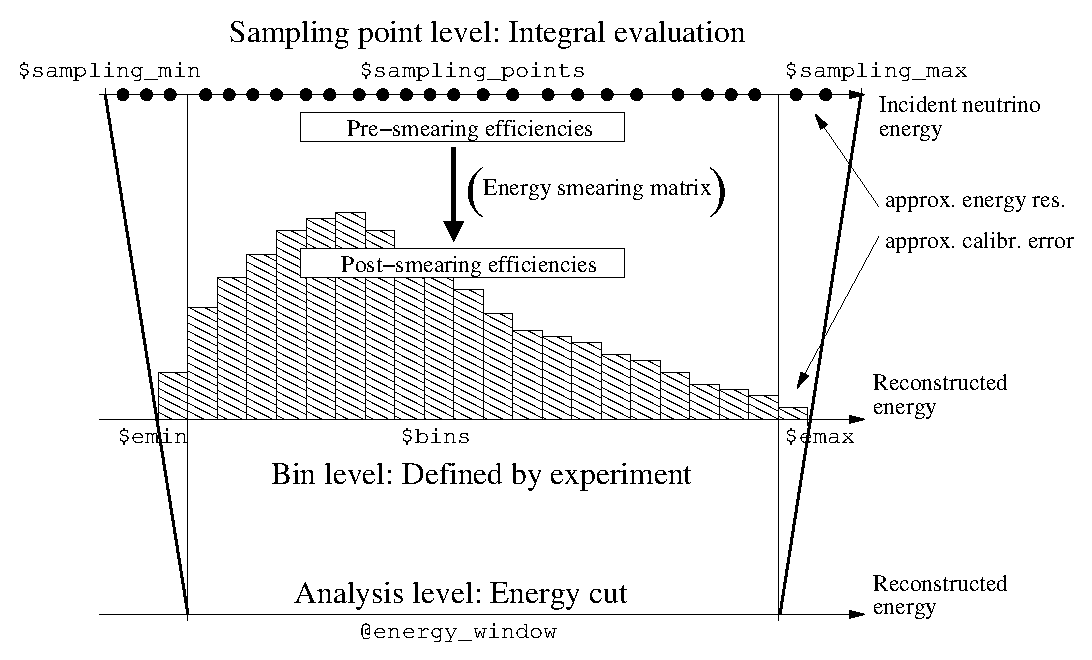
\includegraphics[width=15cm]{energies}
\end{center}
\mycaption{\label{fig:energies} The different evaluation levels for the energy smearing in \GLOBES .}
\end{figure}

Before we come to the calculation algorithms, it is useful to understand
the general evaluation algorithm. As it is illustrated in \figu{energies}, 
\GLOBES\ uses several levels with respect to the energy ranges:
\begin{description}
\item[Sampling point level]
 This level is used internally to evaluate the integrand in \eq~(\ref{eq:simple_int}) at all sampling points. The energy scale is the actual incident neutrino energy $E$. 
For a manual definition of the sampling points, use
\index{aedl}{sampling points@{\tt \$sampling\_points}}
\index{aedl}{sampling min@{\tt \$sampling\_min}}
\index{aedl}{sampling max@{\tt \$sampling\_max}}
\begin{quote}
{\tt
\$sampling\_points = 20\\
\$sampling\_min =          4.0\\
\$sampling\_max =         50.0
}
\end{quote}
for equidistant sampling points. If no values are given for these variables,
they are assumed to be equal to their corresponding counterparts at the bin level,
\ie , \verb+$sampling_points = $bins+, \verb+$sampling_min = $emin+ and
\verb+$sampling_max = $emax+.


Arbitrarily spaced sampling points can 
be specified with 
{\tt \$sampling\_stepsize}\index{aedl}{sampling stepsize@{\tt \$sampling\_stepsize}}
\begin{quote}
{\tt
\$sampling\_stepsize=\{1.0,2.0,3.0,4.0,5.0,...\}
}
\end{quote}
The choice of the sampling point configuration strongly depends on the 
experiment and required accuracy. Ideally, the integrand 
of~\eq~\ref{eq:simple_int} is zero outside the sampling range. If this cannot
be achieved, it is usually sufficient that the sampling range is by about
three times the energy resolution (evaluated at {\tt \$emin} and
{\tt \$emax}, respectively) larger than the bin range. 
The spacing of the sampling points should be somewhat smaller than the 
finest details of the integrand (a factor 
$\simeq 2$ usually is more than enough).



\item[Bin level] This level is determined by the experiment and its analysis. 
Note that energy
bin sizes much smaller than the energy resolution will not improve the results. The energy bin range and the number of energy bins always have to be specified. For the case of large values of the integrand in \eq~(\ref{eq:simple_int}) at the energy range limits, it is recommended to exceed the analysis energy window by about three times the energy calibration error in order 
to avoid cutoff effects.

In order to define a range between $E_\mathrm{min}$
and $E_\mathrm{max}$ divided by a certain number of equidistant bins,
use
\index{aedl}{emax@{\tt \$emax}}
\index{aedl}{emin@{\tt \$emin}}
\index{aedl}{bins@{\tt \$bins}}
\begin{quote}
{\tt
\$emin = 4.0\\
\$emax = 50.0\\
\$bins = 20
}
\end{quote}
For arbitrary bins, use $E_\mathrm{min}$
and $E_\mathrm{max}$ and the size of each bin  $\Delta E_i$:
\begin{quote}
{\tt
\$emin = 4.0\\
\$emax = 50.0\\
\$binsize = \{  15.0 , 5.0 , 20.0, 6.0 \} 
}
\end{quote}
\index{aedl}{binsize@{\tt \$binsize}}
The number of bins will be automatically computed by \GLOBES . Note that the
bin sizes have to add up to the energy range {\tt \$emax}-{\tt \$emin}.

The choices at bin level are mainly determined by optimizing the
performance of the experiment.

\item[Analysis level]
On the analysis level, an energy window can be defined within each rule. For
details, see next chapter.
\end{description}

In general, the energy smearing happens between the sampling point and bin levels, which means that the energy smearing matrix will have {\tt \$sampling\_points} columns and {\tt \$bins} rows. 

As illustrated in \figu{energies}, an interesting feature in combination with the
channels are pre- and post-smearing effects. Pre-smearing effects are taken into account on the sampling point level, and post-smearing effects on the bin level. Examples for these effects are energy 
dependent efficiencies and (non-beam) backgrounds. Efficiencies are multiplicative factors, whereas backgrounds are added to the event rates. These components can be introduced before or after the integration in \eq~(\ref{eq:simple_int}) is done. 
%
\index{aedl}{channel@{\tt channel}!pre smearing efficiencies@{\tt 
"@pre\_smearing\_efficiencies}}%
\index{aedl}{channel@{\tt channel}!pre smearing background@{\tt 
"@pre\_smearing\_background}}%
\index{aedl}{channel@{\tt channel}!post smearing efficiencies@{\tt 
"@post\_smearing\_efficiencies}}%
\index{aedl}{channel@{\tt channel}!post smearing background@{\tt 
"@post\_smearing\_background}}%
%
If they are introduced before, 
we call them
{\tt @pre\_smearing\_efficiencies} or {\tt @pre\_smearing\_background}. 
If they are introduced afterwards, we call them {\tt @post\_smearing\_efficiencies} or {\tt @post\_smearing\_background}.
Note that pre-smearing components are always a function of the incident neutrino energy $E$. Thus, there have to be as  many elements as there are sampling points. 
Examples for pre-smearing quantities are non-beam backgrounds, such as from geophysical neutrinos. The post-smearing components are always a function of the reconstructed neutrino energy $E'$, such as the post-smearing efficiencies $\epsilon_\beta^{\text{IT}}(E')$ in \eq~(\ref{eq:e_res}). Examples for post-smearing efficiencies are cuts and detection threshold functions. All post-smearing components have to have as 
many elements as there are energy bins. Efficiencies are multiplicative 
and their default value is $1$, whereas backgrounds are additive and their default value is $0$. Thus, a more elaborate channel can be defined as
\begin{quote}
{\tt channel(\#channel\_1)<\\
\tb @channel = \#flux : $+$: muon: muon: \#cross: \#energy\\
\tb @pre\_smearing\_background = \{1,2,3,4,5,6,7,8,9,10\}\\
\tb @post\_smearing\_efficiencies = \{0.1,0.2,0.3,0.4,0.5\}\\
>}
\end{quote}
%
\index{aedl}{channel@{\tt channel}!pre smearing efficiencies@{\tt 
"@pre\_smearing\_efficiencies}}
\index{aedl}{channel@{\tt channel}!pre smearing background@{\tt 
"@pre\_smearing\_background}}
\index{aedl}{channel@{\tt channel}!post smearing efficiencies@{\tt 
"@post\_smearing\_efficiencies}}
\index{aedl}{channel@{\tt channel}!post smearing background@{\tt 
"@post\_smearing\_background}}
%
This experiment uses $10$ sampling points and $5$ bins.

In the following subsections we will explain the energy resolution function.
All energy resolution functions are defined within an {\tt energy} environment and can be refered to by {\tt \#name}:
\begin{quote}
  {\tt energy(\#name)<\\
\tb $\ldots$\\
>}
\end{quote}
The individual parameters of the environment will be defined below and depend on the algorithm used.

\subsection{Bin-based automatic energy smearing}

This algorithm is the simplest of the built-in algorithms for the evaluation
of \eq~(\ref{eq:simple_int}). It is applicable to most of the
experiments which can be simulated with \GLOBES .

The key idea is to use a ``flat'' model, \ie\ the integrand 
of~\eq~\ref{eq:simple_int}  is well approximated by being piecewise
constant in each sampling step. This is a good approximation as long as
\begin{itemize}
\item
 No details are lost, \ie\ the spacing of sampling points 
is smaller than the energy resolution.
\item
The edges are treated correctly.
\item
 The neutrino oscillations are slow on a scale of the smapling point distance.
\end{itemize}
In this case, \eq~(\ref{eq:simple_int}) is reduced to
\begin{equation}
\label{eq:algo_one}
n_i^c=N/L^2 \, \sum_{j=1}^N \,  \Phi^c(E_j)\,
P^c(E_j)\,
\sigma^c(E_j)\,
K_i^c(E_j) \, \Delta E_j \,.
\end{equation}
The advantages of this algorithm are obvious: All factors
independent of the oscillation parameters have to be only evaluated once
at values of $E$ which are known in advance, which means that they can be put 
into a look-up table. In addition, the probability
has to be only evaluated at previously known values of the energy, which
makes it possible to compute the transition amplitudes for all channels
simultaneously. One assumption is that all involved factors are piece-wise
constant, \ie, they hardly change within each bin. This 
assumption seems to be very restrictive, which is however not quite correct.
First of all, if one analyzes simulated data (which are simulated with the same algorithm), the errors
will cancel between the simulated and fitted data. Second, and more important,
this algorithm is just a very basic integration routine\footnote{It is planned 
for the future to implement something like a Gau\ss-Kronrod scheme as an
alternative here.} and converges to the true result for decreasing step size.
Thus if the number of sampling points is large enough this algorithm is very
accurate. Bin-based energy smearing is selected by
%
\index{aedl}{energy@{\tt energy}!type@{\tt "@type}}
%
\begin{quote}
{\tt \tb @type = 1}
\end{quote}
within the {\tt \#energy} environment.
The computation of the bin kernel $K_i^c$ is performed
by \GLOBES. Thus, it requires that the number of bins
{\tt \$bins} and the minimum energy {\tt \$emin} and maximum energy {\tt \$emax} are given in case of equidistant bins.
%
\index{norm}{Energy!resolution}
\index{norm}{Energy!resolution function}
%
As far as the parameterization for the energy resolution function 
$R^c(E,E')$ in \eq~(\ref{eq:kernel}) is concerned, the algorithm uses
a Gau\ss ian
\begin{equation}
R^c(E,E')=\frac{1}{\sigma(E)\,\sqrt{2\pi}}\,e^{-\frac{(E-E')^2}{2\sigma^2(E)}} \, .
\end{equation} 
%
\index{aedl}{energy@{\tt energy}!sigma function@{\tt "@sigma\_function}}
%
There are several energy resolution functions available, where by default
{\tt \#standard} is used:
\begin{quote}
{\tt \tb @sigma\_function = \#standard} 
\end{quote}
%
\index{aedl}{energy@{\tt energy}!standard@{\tt \#standard}}
%
The energy resolution function {\tt \#standard} is defined by
\begin{equation}
\label{eq:sigma_e}
\sigma(E)=\alpha\cdot E + \beta \cdot \sqrt{E} +\gamma\, ,
\end{equation}
where the parameters $\alpha, \beta$ and $\gamma$ are provided by the user:
\begin{quote}
{\tt \tb @sigma\_e = \{0.15, 0.0, 0.0\}}
\end{quote}
Currently, another possible choice for {\tt @sigma\_function} is {\tt \#inverse\_beta},
%
\index{aedl}{energy@{\tt energy}!inverse beta@{\tt \#inverse\_beta}}
%
which only uses the parameter $\alpha$. It is defined by
\begin{equation}
\sigma(E)= \left\{\begin{array}{cl}
 \alpha \cdot \sqrt{1000}^{-1}\,\sqrt{x-8\cdot10^{-4}}\,,&\mathrm{for}\,\, 
x>1.8\cdot10^{-3}\\
\alpha\cdot10^{-3} \,,&\mathrm{for}\,\, x \leq 1.8\cdot10^{-3}
\end{array} \right.
\end{equation}
The somewhat complicated form is due to the fact that inverse $\beta$-decay
has a neutrino threshold of $1.8\,\mathrm{MeV}$ and that a neutrino
at threshold already produces $\simeq 1\,\mathrm{MeV}$ visible energy in
the detector (for more details see \eg~\cite{Huber:2003pm}). 

In the actual implementation of the algorithm,  the sum in \eq~(\ref{eq:algo_one}) is only evaluated
 for the $E_j$'s with $K(E_j)$ 
above a certain threshold, which is, by default, $10^{-7}$. 
This threshold is defined at compilation time. 

Eventually,  a complete energy resolution definition with bin-based
automatic energy smearing is, for example,
\begin{quote}
{\tt energy(\#name)<\\
\tb @type = 1\\
\tb @sigma\_function = \#standard\\
\tb @sigma\_e = \{0.15 ,0.0 ,0.0\}\\
>
}
\end{quote}

\subsection{Low-pass filter}

In order to ensure that very fast oscillations do not lead to 
aliasing,\index{norm}{Aliasing}
it is possible to impose a low-pass filter already during the calculation
of the probabilities itself. This highly
experimental feature will be called ``filter''\index{norm}{Filter} in the following. 
The calculation of oscillation
probabilities is, in principle, a computation of phase differences. Restricting the maximum admissible size of those phase differences effectively filters
the high frequency component of the oscillation probability. This idea is
implemented according to
\begin{eqnarray}
\label{eq:filter_a}
P_{\alpha\beta}(E)&=&\sum_{ij}
U_{\alpha j} U^*_{\beta j} U^*_{\alpha i} U_{\beta i} 
e^{-i\Phi_{ij}}\times 
e^{ -\Phi_{ij}^2/\sigma_f(E)^2 }\,,
\end{eqnarray}
where $\Phi_{ij}:=\Delta m_{ij}^2 L/2E$ is the usual phase difference and
the last term is a Gau\ss ian filter with width $\sigma_f(E)$. Choosing
$\sigma_f(E):=\sigma_f^0 \cdot E$ ensures that this filter behaves 
approximately as an energy resolution function with constant width 
$\sigma_e=\sqrt{2}/\sigma_f^0$, \ie\
\begin{equation}
\label{eq:filter_b}
\int d\tilde E\quad P(\tilde E) \frac{1}{\sigma_e\,\sqrt{2\pi}}\,
e^{-\frac{(E-\tilde E)^2}{2\sigma^2_e}}\,.
\end{equation}
The relationship between \eqs~\eqref{eq:filter_a} and~\eqref{eq:filter_b}
is not obvious and connected to the properties of $P_{\alpha\beta}$: 
see \Refs~\cite{Kiers:1996zj,Giunti:2003ax}. This feature works \emph{only} 
for vacuum and constant densities and is controlled
by the filer state variable. In addition, $\sigma_e$ is set by the filter value variable:
\index{aedl}{filter state@{\tt \$filter\_state}}
\index{aedl}{filter value@{\tt \$filter\_value}}
\begin{quote}
{\tt
\$filter\_state = 1\\
\$filter\_value = 2.0\\
}
\end{quote}
would switch the filter feature on and set the width to $2.0\,\mathrm{GeV}$.
The setting of {\tt \$filter\_state} is ignored whenever a density profile
with more than one layer is used. 

\index{aedl}{energy@{\tt energy}!type@{\tt  "@type}}
With a type 1 ({\tt @type = 1}) energy resolution 
function, $\sigma_e$ contributes to the energy resolution function 
of the detector $\sigma_c(E)$ according to
\begin{equation}
\sigma_{\mathrm{eff}}(E)^2\simeq \sigma_e^2 + \sigma_c(E)^2\,.
\end{equation} 
Sometimes this behavior is unwanted, and therefore one can try to 
'subtract' the filtering from the energy resolution function by splitting 
the energy resolution function $\sigma(E)_{\mathrm{eff}}$ into
two parts by
\begin{equation}
\sigma_{\mathrm{eff}}(E)^2=\underbrace{\sigma_c(E)^2-\sigma_e^2}_
{\tilde\sigma^2_c(E)}+\sigma_e^2\,,
\end{equation}
where the truncated energy resolution function $\tilde\sigma_c(E)$ 
is used instead of $\sigma_c(E)$ in computing the
smearing data. Thus one obtains as effective energy resolution
\begin{equation}
\sigma_{\mathrm{eff}}(E)^2\simeq \sigma_c(E)^2\,.
\end{equation} 
This scheme is used by choosing as type for the energy resolution
\begin{quote}
{\tt
@type = 2
}
\end{quote}

\subsection{Manual energy smearing}

In some cases, one may want to use the output of a detector Monte Carlo simulation
directly. Then one can use ''manual'' energy smearing instead  of the
automatic energy smearing algorithms. 

The energy smearing matrix $K_{ij}$ has {\tt \$bins} rows and {\tt \$sampling\_points} columns, which are numbered from $0$ to {\tt \$bins}$-1$ resp.\ {\tt \$sampling\_points}$-1$. It is equivalent to the 
bin- and sampling-point-based kernel in \eq~(\ref{eq:kernel}):
\begin{equation}
K_{ij} = K_i^c(E) |_{E=E_j},
\label{equ:ematrix}
\end{equation}
where $E_j$ is the energy of the $j$th sampling point. In general, many of the entries in this matrix are zero, which means that it is convenient to evaluate the integrand in \eq~(\ref{eq:simple_int}) only at positions where
$K_{ij}$ is non-zero. The corresponding ``sampling range'' of non-zero matrix entries  in $K_{ij}$ for the $i$th energy bin is defined to run from
column $k_l^i$ (``lower index'') to column $k_u^i$ (``upper index'').
An example for a smearing matrix is
\begin{equation}
K_{ij} =   \underbrace{ \left( \begin{array}{cccccccccc} 
a_{00} & a_{01} & a_{02} & a_{03} &  &  &  &  &  & \\
a_{10} & a_{11} & a_{12} & a_{13} & a_{14} &  &  &  &  &  \\
 & a_{21} & a_{22} & a_{23} & a_{24} & a_{25} &  &  &  &  \\
 &  & a_{32} & a_{33} & a_{34} & a_{35} & a_{36} &  &  &  \\
 &  &  & a_{43} & a_{44} & a_{45} & a_{46} & a_{47} &  &  \\
& & & \uparrow  & & \ddots & & \uparrow & & \\
& & & k_l^i & & & & k_u^i & & \\ 
\end{array}\right) }_{\mathtt{\$sampling\_points}  \, \, \mathrm{columns}} \quad \leftarrow \quad \footnotesize{\mathtt{\$bins} \, \, \mathrm{rows}} \, ,
\end{equation}
where the unshown entries are zero. Thus, the values of $K_{ij}$ have to be specified between $k_l^i$ and $k_u^i$ in the form $\{ k_l^i,k_u^i, K_{i \, k_l^i}, K_{i k_l^i+1} , \hdots , K_{i k_u^i} \}$:
\index{aedl}{energy@{\tt energy}!energy@{\tt "@energy}}
\begin{quote}
{\tt 
energy(\#name)<\\
\tb @energy =   \{0,2, 0.8634265, 0.0682827,     4e-06\}:\\
\tb\tb \{0,4, 0.1507103, 0.6965592, 0.1507103,   0.00101,     1e-07\}:\\
\tb\tb $\ldots$\\
\tb\tb \{40,42, 0.1507103, 0.6965592, 0.1507103\};\\
>
}
\end{quote}
The last line has to be terminated by a semicolon `;'.
Note that the sum of all entries in each {\em column} should be equal 
to unity,
since all of the incoming neutrinos should be assigned to energy bins. In many practical cases, however, the definition of the energy smearing can
lead to sums smaller than unity, such as in the case of truncated Gau\ss ian
distributions. The sum of entries in each {\em row} is not defined, since the events might be unevently distributed into the energy bins
according to the energy resolution function.

\index{aedl}{energy@{\tt energy}|)}
\index{norm}{Energy!resolution|)}
%%%%%%%%%%%%%%%%%%%%%%%%%%%%%%%%%%%%%%%%%%%%%%%%%%%%%%%%%%%%%%%%%%%%%%%%%%%%
\section{Rules and the treatment of systematics}
\label{sec:rules}

\index{aedl}{rule@{\tt rule}|(}
The set of rules\index{norm}{Rule} for an experiment is the final 
link between the event rate computation and the statistical analysis. 
The information in the rules
specifies how the $\chi^2$ is computed based upon the raw event rates 
given by the channels and possible systematical errors. 
Therefore a rule has two parts: The first part describes how signal and 
background events are composed out of the channels, and the second part
specifies which systematical errors are considered, as well as their values.
%
For a rule, the splitting
into signal and background is useful for the treatment of systematics, as we will se later. Each rule will lead to a $\Delta \chi^2$-value,
which means that all $\Delta \chi^2$'s of the different rules will be added
for the whole experiment. Within each rule, the event rates are added, and
the systematics is considered to be independent of the other rules (unless user-defined
systematics specifies a dependence).
Thus, it is convenient to combine the previously defined channels for different
oscillation patterns and interaction types into one logical construction,
which is the rule. For example, a superbeam usually has two rules: One for
the $\nu_e$-appearance rates, and one for the $\nu_\mu$-disappearance rates.
 In each case, contributions of several interaction types, as well as from
 the $\nu_e$-contamination of the beam will lead to a number of contributing signal and background event channels.

For each rule, the signal event rate $s_i$ in the $i$th bin can be composed 
out of one or more channels according to 
\begin{equation}
s_i=\alpha_{c_{s1}}\cdot n_i^{c_{s1}}\,+\,\alpha_{c_{s2}}\cdot n_i^{c_{s2}}\,+\,\ldots
\end{equation}
where the $\alpha$'s are overall normalization factors/efficiencies
 determined by the properties of the detector. Note that bin-based (energy-dependent) efficiencies can be defined with the post-smearing efficiencies in the last section. 
In addition, note that in most cases, it makes sense to have only one 
signal channel and to assign all sorts of perturbations to the background. 
%
Similarly, the background event rate $b_i$ in the $i$th bin can be composed
out of one or more channels:
\begin{equation}
b_i=\beta_{c_{b1}}\cdot n_i^{c_{b1}}\,+\,\beta_{c_{b2}}\cdot n_i^{c_{b2}}\,+\,\ldots \, ,
\end{equation}
where the channels can be any combination of the ones in the signal rate and 
additional ones. The background normalization factors very often have
a specific meaning. For example, they may correspond to a fraction
of mis-identified events (charge or flavor mis-identification).
%
\index{aedl}{rule@{\tt rule}!signal@{\tt "@signal}}
\index{aedl}{rule@{\tt rule}!background@{\tt "@background}}
%
These basic building blocks of each rule are, within the rule environment,
for example defined by
\begin{quote}
{\tt \tb @signal = 0.5 @ \#channel\_1\\
\tb @background = 0.001 @ \#channel\_2 :  0.005 @ \#channel\_3
}
\end{quote}

For the analysis of the systematical errors, the so called 
 ``pull method'' is used~\cite{Fogli:2002pt}\footnote{In fact the pull 
method was employed already in \Ref~\cite{Huber:2002mx} before 
\Ref~\cite{Fogli:2002pt} appeared.}. 
For the pull method, $k$ systematical errors are included by introducing 
$k$ additional variables $\zeta_k$, which are the 
so-called ``nuisance parameters''. 
The nuisance parameters describe the dependence 
of the event rates on the various sources of systematical errors. 
For example, an error on the total 
normalization is included by multiplying the expected number of events in 
each bin by a factor $(1+\zeta_1)$. The variation of $\zeta_1$ in the fit is
constrained by adding a penalty $p_1$ to the $\chi^2$-function. In case 
of a  Gau\ss ian distributed systematical error, this penalty is 
given by
\begin{equation}
\label{eq:penalty}
p_i=\frac{\zeta_i^2}{\sigma_{\zeta_i}^2}\,,
\end{equation}
where $\sigma_{\zeta_i}$ is the standard 
deviation of the corresponding nuisance parameter. In the following,
we will refer to the  standard deviation as
the ``error'', since it corresponds to the actual systematical uncertainty.
Note that the central values of all penalties are zero in \GLOBES\ 3.0 and higher. 
The resulting $\chi^2$ is then minimized with respect to all nuisance 
parameters $\zeta_i$, which leads to $\chi^2_\mathrm{pull}$
\begin{equation}
\chi^2_\mathrm{pull}(\boldsymbol{\lambda}):=\min_{\{\zeta_i\} } \,\, \left( 
\chi^2(\boldsymbol{\lambda},
\zeta_1, \ldots, \zeta_k)+ \sum_{j=1}^{k} p_j(\zeta_j)\right)\,.
\end{equation}
Here $\boldsymbol{\lambda}$ refers to the oscillation parameters 
including the matter density
$\rho$. One advantage of the pull method is that whenever the number $N$ of 
data points is much larger than $k$, it is numerically easier to compute 
$\chi^2_\mathrm{pull}$ than to invert the $N\times N$ covariance matrix. For
the experiments considered here, $N$ is typically $20$ and $k\sim 4$, 
which means that the pull method is numerically much faster. Moreover,
 it is more flexible and  allows the inclusion of systematical errors 
also for a Poissonian $\chi^2$-function.
In \Ref~\cite{Fogli:2002pt}, it has been demonstrated that the pull method 
and the covariance based approach are equivalent for a Gau\ss ian and 
linear model. In general,
there is a separate $(\chi^2_\mathrm{pull})^r$ for each rule $r$, 
\ie , pair of signal and background spectra, with a separate set of 
nuisance parameters $\zeta_i^r$. Thus, $\chi^2_\mathrm{pull}$
is the sum of all individual  $(\chi^2_\mathrm{pull})^r$'s.
By the minimization, the dependence on the $k$ nuisance parameters is eliminated  from $\chi^2_\mathrm{pull}$. 

Now, we can introduce the different systematical errors. 
The two most important and
most easily parameterized systematical errors are the normalization 
and energy calibration errors. These errors are assumed to be independent between the signal events and the background events, which means that
this systematics treatment defines the grouping into signal or background.
The implementation of the normalization error
is straightforward:
\begin{equation}
s_i(a):=(1+a)\cdot s_i
\end{equation} 
with an analogous definition for the background events. Here, $a$ is the ``nuisance'' parameter, which will be minimized over later.

For the parameterization of an energy calibration error, two possibilities
are implemented. The first one (method ``T'') is somewhat simpler, 
whereas the second one (method ``C'')
is more accurate, but it requires a careful choice of parameters. 
The first option (method ``T'') is\footnote{Note that this behaviour
has slightly changed compared to previous \GLOBES\ releases.}
\begin{equation}
  s_i(a,b) \equiv s_i(a)+b\cdot s_i \, (E'_i - \bar{E'}) / (E'_\mathrm{max}-E'_\mathrm{min}),
\end{equation}
where $E'_\mathrm{min}$ and $E'_\mathrm{max}$ correspond to {\tt \$emin} and
{\tt \$emax}, $\bar{E'} = \tfrac{1}{2} (E'_\mathrm{max}+E'_\mathrm{min})$ is
the median of this energy interval, and $E'_i$ is the mean (reconstructed)
energy of the $i$th bin.
This method is often refered to as a ``tilt'' of the
spectrum, since it describes a linear distortion 
of the event rate spectrum.
%Note that this definition of a tilt makes
%only sense in combination with a large enough normalization error, since
%the tilt may also affect the normalization. 
%
The second option (method ``C'') is closer to an actual energy
calibration error, which means that one should test this option whenever
one suspects a large impact of this systematical error.
It is based upon replacing the events in the $i$th bin
by the ones at the energy $(1+b)\cdot E'_i$. If the target energy does not exactly hit
a (discrete) bin energy $E_k$, linear interpolation is used. We use the following approximation:
\begin{eqnarray}
s_i(a,b)&=& (1+b)\cdot \left[ \left( s_{k+1}(a)-s_k(a) \right)\cdot (\delta-k) +s_k(a) \right] \,,
  \label{eq:Ecalib} \\
\delta&=&b\cdot(i+t_0+ 1/2)+i\,,\nonumber\\
k&=& \mathrm{div}(\delta,1)\,,\nonumber\\
t_0&=&E'_\mathrm{min}/\Delta E_0\,.\nonumber
\end{eqnarray}
Here, $\Delta E_0$ is the bin width ({\tt \$emax}-{\tt \$emin})/{\tt \$bins},
and ``div'' refers to the integer part of the division. It is important
to keep in mind that this definition of the energy calibration error 
makes sense only for constant bin widths, so the corresponding $\chi^2$
functions should not be used in conjunction with the {\tt \$binwidth} directive.
The factor $(1+b)$ in \eq~\eqref{eq:Ecalib} comes from a renormalization of
the bin width, since also the bin width is altered by the replacement of
the energies. Furthermore, special attention has to be given to the limits
 $k<1$ or $k+1>N_\mathrm{bins}$, since there $s_k$ or $s_{k+1}$ may not have been calculated. By default, it is assumed that $s_k$ is
zero in those cases. However, if the event rates are still large at
the limits, this will introduce errors, leading to a wrong
estimate of the impact of the calibration error. In this case,
one should truncate the analysis range by a few bins at the boundaries
and thus ensure that only those $s_i$, whose index
$k$ is within the range $0,\ldots, N_\mathrm{bins}-1$ (\cf, \figu{energies}), are used.
Therefore, it is possible to constrain the analysis energy range 
with each rule to an energy window\index{norm}{Energy!window}:
\index{aedl}{rule@{\tt rule}!energy window@{\tt "@energy\_window}}
\begin{quote}
{\tt 
\tb @energy\_window = 4.0 : 50.0 
}
\end{quote}
The default energy window is given by the minimal and maximal reconstructed
energies {\tt \$emin} and {\tt \$emax}. To be on the safe side, one should
reduce the analysis window compared to the bin range on each side by about
three times the energy calibration error.

%%%%%%%%%%%%%%%%%%%%%%%%%%%%%%%%%%%%%%%%%%%%%%%%%%%%%%%%%%%
\begin{table}[t!]
\begin{center}
\begin{tabular}[h]{|lccccccl|}
\hline
Systematics function &$a$&$b$&$c$&$d$&Tilt/Calibr.& Dim. & Remarks\\
\hline
\hline
\multicolumn{8}{|l|}{{\bf Standard systematics:}} \\
{\tt chiSpectrumTilt} &+&+&+&+&T&0&Systematics with tilt\\
{\tt chiNoSysSpectrum} &-&-&-&-&-&2&No systematics, but\\
 & & & & & & & spectral information \\
{\tt chiTotalRatesTilt} &+&+&+&+&T&4&Total rates\\
{\tt chiSpectrumOnly} & $\infty$ &-& $\infty$ &-&-&7&Spectrum only\\
{\tt chiNoSysTotalRates} &-&-&-&-&-&8&Total rates, no syst.\\
{\tt chiSpectrumCalib} &+&+&+&+&C&9&Systematics with calibr.\\
\hline\multicolumn{8}{|l|}{{\bf User-defined systematics:}} \\
{\tt chiZero} & - & - & - & - & - & n/a & Passive rule\\
 & & & & & & & ($\chi^2$ returns zero) \\
Any other name & \multicolumn{5}{c}{User-defined behavior} & n/a & User-defined syst. \\
\hline
\end{tabular}
\mycaption[Table of error dimensions]{\label{tab:error_dim}
Possible systematics $\chi^2$ functions  in \GLOBES\ and their meaning. 
If a parameter is designated with $+$, it will
be marginalized over, and therefore the corresponding error needs to 
have a non-zero value. In the cases with ``total rates'' in the remarks, 
the summation over the bins is performed \emph{before} computing 
the $\chi^2$, \ie, no spectral information is used. 
The function {\tt chiSpectrumOnly} leaves the 
normalization free ($\sigma_a=\sigma_c=\infty$), and therefore 
only the spectral information is used. As a consequence,
the settings for the normalization error will be ignored (designated 
with the symbol $\infty$). In addition, the corresponding error
dimension from earlier versions of \GLOBES\ is shown in the column ``Dim.''.
 }
\end{center}
%\index{aedl}{{\tt rule}!errordim@{\tt "@errordim}} 
\index{norm}{Systematics function} 
\end{table} 
%%%%%%%%%%%%%%%%%%%%%%%%%%%%%%%%%%%%%%%%%%%%%%%%%%%%%%%%%%%%%%

Eventually, the total event rate $x_i$ in a bin $i$ is given by
\begin{equation}
x_i(a,b,c,d)=s_i(a,b)+b_i(c,d) \, ,
\end{equation}
and is thus a function of four parameters. 
The four parameters $a,b,c,d$ have been introduced in order to describe
systematical uncertainties and are the nuisance parameters.
Each of the four parameters has a corresponding systematical error.
% The central values for all of
% the four parameters have to be always defined for built-in systematics. 
They are called  signal normalization ($a$), signal tilt/calibration ($b$), 
background  normalization ($c$) and
background tilt/calibration ($d$). Their default (central) values are
zero.\footnote{The old parameter {\tt @backgroundcenter} should not be used anymore.
A background normalization center of 1.0 will be interpreted as zero central value.}
% \begin{equation}
% a=1\,,\quad b=0\,,\quad c={\tt not \, \, assigned}\,,\quad d=0\,.
% \end{equation}
% Thus, for the background normalization $c$, the value has to be specified 
% in \emph{either} case. 
The errors for the normalization and the 
values of tilt/calibration are always regarded
as pairs, \ie, they are given in the form {\tt normalization :\ tilt}.
For example, we have
\index{aedl}{rule@{\tt rule}!signal error@{\tt "@signalerror}}
\index{aedl}{rule@{\tt rule}!background error@{\tt "@backgrounderror}}
%\index{aedl}{{\tt rule}!background center@{\tt "@backgroundcenter}}
\begin{quote}
{\tt
\tb @signalerror =       0.001  :       0.01\\
%\tb @backgroundcenter =  0.1 :       0.0\\
\tb @backgrounderror =   0.001 :       0.01
}
\end{quote}
% There is no {\tt @signalcenter} in this definition, 
% since by default the central value for the
% signal normalization is $1$ and the central value for the tilt/calibration 
% is $0$.  
%
The user has the possibility to choose the set $\{\zeta_i\}$ of nuisance 
parameters which are minimized over. This choice is specified with the 
systematics functions {\tt sys\_on\_function} and {\tt sys\_off\_function}
corresponding two systematics modes ``systematics on'' and ``systematics off''.\footnote{In earlier
versions before \GLOBES\ 3.0 the ``error dimension'' was used. The corresponding
parameters {\tt errordim\_sys\_on} and {\tt errordim\_sys\_off} are still supported
but should not be used anymore.}
\index{aedl}{rule@{\tt rule}!sys on function@{\tt "@sys\_on\_function}}
\index{aedl}{rule@{\tt rule}!sys off function@{\tt "@sys\_off\_function}}
\index{norm}{Systematics function}
The different  possibilities are shown in
\Tab~\ref{tab:error_dim}. Since the dual systematics modes define the behavior
of the experiment for systematics on and off, it is useful to have a matching pair of 
systematics functions for each rule 
(see also~\Sec~\ref{sec:systematics}). The signal and background errors specified
by {\tt @signalerror} and  {\tt @backgrounderror} will then be used, if applicable.
For example, one may define 
\begin{quote}
{\tt
\tb @signalerror =       0.001  :       0.01\\
\tb @backgrounderror =   0.001 :       0.01 \\
\tb @sys\_on\_function = "chiSpectrumTilt"  \\
\tb @sys\_off\_function = "chiNoSysSpectrum"  
}
\end{quote}

For user-defined systematics \index{norm}{User-defined systematics}
(see, \Sec~\ref{sec:userchi}), one can use arbitrary names
for the systematics functions which are not pre-defined. In this case,
one would specify the systematical errors in lists, such as
\index{aedl}{rule@{\tt rule}!sys on errors@{\tt "@sys\_on\_errors}}
\index{aedl}{rule@{\tt rule}!sys off errors@{\tt "@sys\_off\_errors}}
\begin{quote}
{\tt
\tb @sys\_on\_function = "chiMySystematics"  \\
\tb @sys\_on\_errors = \{ 0.2, 0.3, 0.5 \}~// Uses three syst. errors \\
\tb @sys\_off\_function = "chiNoSysSpectrum"  \\
\tb @sys\_off\_errors = \{ \}
}
\end{quote}
Note that here, the systematics on and systematics off models can be used 
as two different, fully functional systematics modes with different systematical
errors. The interpretation of the systematical errors in {\tt @sys\_on\_errors} and
{\tt @sys\_off\_errors} is left to the application software code and the user.
In addition, the application software has to register the user-defined systematics $\chi^2$
function with \GLB{DefineChiFunction} and uniquely identify the name
given by {\tt @sys\_on\_function} or {\tt @sys\_off\_function} to avoid
confusing different systematics routines. In addition, it is possible to define
a rule with passive systematics using {\tt glbChiZero}. In this case, the
contribution to $\chi^2$ from this rule will always be set to zero, but
the corresponding rate vectors will be calculated and provided for indirect access
by other systematics functions. For example, a reactor experiment with correlated
systematics between near and far detectors may define the user-defined systematics
{\tt chiReactor} for the far detector and use {\tt chiZero} for the near detector.
The routine assigned to the far detector will then perform the $\chi^2$ calculation,
which, of course, also involves the rates of the near detector. However, defining
{\tt chiReactor} in both the near and far detectors would result in a double call
of the $\chi^2$ function, \ie, the resulting $\chi^2$ would be too large by a factor two
and the program would be slower by a factor of two.
Note that mixed declarations of {\tt @sys\_on\_errors}, {\tt @sys\_off\_errors}, {\tt @signalerror}, and
{\tt @backgrounderror} are possible. In this case, {\tt @sys\_on\_errors} and {\tt @sys\_off\_errors}
have priority. If one or both of these are not present, {\tt @signalerror} or
{\tt @backgrounderror} will be used.

Eventually, a complete rule may look like this:
\begin{quote}
{\tt rule(\#rule\_1)<\\
\tb @signal = 0.5 @ \#channel\_1\\
\tb @background = 0.001 @ \#channel\_2 :\ 0.005 @ \#channel\_3\\
\tb @signalerror =       0.001  :\ 0.01\\
\tb @backgrounderror =   0.001 :\ 0.01\\
\tb @sys\_on\_function = "chiSpectrumTilt"  \\
\tb @sys\_off\_function = "chiNoSysSpectrum"  \\
\tb @energy\_window = 4.0 :\ 50.0 \\
>}
\end{quote}
\index{aedl}{rule@{\tt rule}|)}

% THIS PART HAS GAINED IMPORTANCE AND THEREFORE BEEN EXPLAINED ALREADY IN THE LAST CHAPTER!
%
%%%%%%%%%%%%%%%%%%%%%%%%%%%%%%%%%%%%%%%%%%%%%%%%%%%%%%%%%%%%
% \section{Version control in \AEDL\ files}
% \label{sec:aedl_versioning}
% \index{norm}{Version control}
% 
% In order to avoid problems which come from different
% versions of \GLOBES\ and \AEDL\ files, it is possible to use in each 
% \AEDL\ file a version number. For example, it may correspond to the  minimum version number of the \GLOBES\ package with which it works. Set the
% {\tt \$version}\index{aedl}{version@{\tt \$version}} by
% \begin{quote}
% {\tt \$version="1.8.1"}
% \end{quote}
% This information can be accessed by the versioning functions as described in~\Sec~\ref{sec:versioning}.
% \index{norm}{AEDL@\AEDL|)}

%%%%%%%%%%%%%%%%%%%%%%%%%%%%%%%%%%%%%%%%%%%%%%%%%%%%%%%%%%%%%%%%%%%%%%%
%%%%%%%%%%%%%%%%%%%%%%%%%%%%%%%%%%%%%%%%%%%%%%%%%%%%%%%%%%%%%%%%%%%%%%%
\chapter{Testing \& debugging of \AEDL\ files}
\label{chap:exp_def}

\AEDL\ is a powerful language to describe a variety 
of different experiments.
This chapter demonstrates how to test an \AEDL\ file in order to check
if it really describes a given experiment. 
For this application, the \GLOBES\ package contains the program
{\tt globes}\index{norm}{globes@{\tt globes}}. It can either be 
regarded as an \AEDL\ debugger, or as a simple command-line oriented tool to convert the rather  abstract \AEDL\ experiment description into more accessible event rates.

\section{Basic usage of the {\tt globes} binary}
\label{sec:globes_basics}

The {\tt globes}\index{norm}{globes@{\tt globes}} binary is installed 
together with the library\index{norm}{libglobes@{\tt libglobes}}, but
into the directory {\tt \$prefix/bin/}. In order to use the {\tt globes} 
utility, this directory has to be in the path of the shell used to call the program.\footnote{This is automatically the case if
no options are given to {\tt configure}, and {\tt make install} was 
executed with root-privilege, \ie, a standard installation was done.}

As an argument, {\tt globes} takes a {\tt .glb}-file. While parsing it,
it prints any warnings and errors which have occured during reading the file. Then it uses the experiment description in the file to compute the event rates at a certain point in parameter space. Finally, it displays the result based on the options used to call {\tt globes}. 
The options of {\tt globes} follow the GNU standard. Thus, there
is a {\tt \verb+--+help} option to display all other options 
together with short descriptions.

\index{norm}{globes@{\tt globes}!oscillation parameters}
Calling {\tt globes} without any options and with a {\tt .glb}-file as argument produces an event summary at rule level. In this case,  
the full experiment description in the file is taken into account, \ie, all efficiencies, backgrounds, and energy resolution effects. 
Thus, the returned event rates are the ones which will be actually 
used to compute the $\chi^2$ later. By default, the oscillation parameters used to calculate the transition probability are
\begin{eqnarray}
\label{eq:globes_params}
\sin^22\theta_{12}=0.8&\quad&\Delta m^2_{21}=7\cdot10^{-5}
\,\mathrm{eV}^2\,,\nonumber\\
\sin^22\theta_{23}=1.0&\quad&\Delta m^2_{31}=3\cdot10^{-3}
\,\mathrm{eV}^2\,,\nonumber\\
\delta=0&\quad&\sin^22\theta_{13}=0.1\,.\
\end{eqnarray}
Of course, it is possible to change these default values either by using the
option {\tt -p} on a call by call basis, or by setting the environment variable
{\tt GLB\_CENTRAL\_VALUES}:
%
\index{norm}{GLB CENTRAL VALUES@{\tt GLB\_CENTRAL\_VALUES}} 
\index{norm}{Environment variables!GLB CENTRAL VALUES@{\tt GLB\_CENTRAL\_VALUES}}
%
\begin{quote}
{\tt
globes -p'0.55,0,0.785,0,0.0008,0.0025'\\
globes \verb+--+parameters='0.55,0,0.785,0,0.0008,0.0025'
}
\end{quote}
For example, {\tt GLB\_CENTRAL\_VALUES} can be defined
within the shell session or in the shell profile:
\begin{quote}
{\tt
export GLB\_CENTRAL\_VALUES='0.55,0,0.785,0,0.0008,0.0025'
}
\end{quote}
Note that in the case of additional non-standard parameters, these will just to 
be included at the end of these lists.
Furthermore it is possible to switch off oscillations with the {\tt -N} option and to switch them on again with {\tt -O} (the default). The effect of {\tt -N} is the same as to use {\tt NOSC\_} in all oscillation channels.
Thi feature is useful if one wants to normalize an expriment flux if
the number of un-oscillated events is given.

\index{norm}{globes@{\tt globes}!warnings}
\index{norm}{globes@{\tt globes}!errors}
\index{norm}{globes@{\tt globes}!verbosity}
The \AEDL\ parser and interpreter have basically three levels of messages to
the user: Warnings, errors and fatal errors. 
Fatal errors are always reported and lead to a 
program exit with status '1'. Usually only errors and no warnings
are reported. The verbosity level can be chosen by the {\tt -v} option, where {\tt -v1} is default, \ie, only errors and fatal errors are reported. The level {-v0} corresponds to reporting fatal errors only, and {\tt -v2} will print warnings in addition to fatal errors. It is recommended
to test any new {\tt .glb}-file with {\tt -v2} to check the warnings at least once, and to decide whether there is a problem to be fixed. With {\tt -v3} all files read by {\tt globes} are displayed together with their path, and with  {\tt -v4} all files which have been attempted to be read are shown.
These two setting are useful to clarify path resolution issues and shadowing
of file names.

\section{Testing \AEDL\ files}
\label{sec:globes_test}

In the process of defining a new experiment, the default output of {\tt globes} at rule level is the final step. However, in order to arrive 
at this level it is often necessary to review the intermediate steps in the event rate calculation. The {\tt globes} utility offers many possibilities to do this based on the rate access functions as described in \Sec~\ref{sec:event_rates}.

\index{norm}{globes@{\tt globes}!total rates}
\index{norm}{globes@{\tt globes}!spectral rates}
By default, {\tt globes} returns total rates corresponding to the 
{\tt -t} option. This can be changed to
to a full spectrum by using {\tt -s}. The spectral rates are shown in a
table where the first column always gives the central energy of the
corresponding bin or the sampling point.

If there is more than one experiment in a file, \ie, there is at least one 
{\tt \#NEXT\#} command, only the event rates for one experiment will be shown.  This experiment can be chosen with the {\tt -e} option, which takes 
as a mandatory argument the number of the experiment (starting with zero).
The default is {\tt -e0}.

\subsection*{Channel level}
\index{norm}{globes@{\tt globes}!channel rates}

As a first step, one may want to check if each channel produces the 
anticipated output. Channel rates are returned if the {\tt -c} option 
is used.
This option takes as an optional argument the channel number 
(starting at zero). If no argument is given all channels are displayed.
By default, the sum of the event rates in each channel is shown. Each 
column has as first line the same channel name as in the file. 

It is also possible to switch off one detector effect after the other. 
First, one can switch off the post-smearing efficiencies ({\tt -f}) and the 
post-smearing backgrounds ({\tt -g}). Next, one can switch off the 
energy resolution function with ({\tt -b}) and view the rates before
smearing. If the {\tt -s} option is also used, the number of
lines in the output will be given by {\tt \$sampling\_points}.
Another effect of the {\tt -b} option is that the post-smearing efficiencies
and backgrounds are no longer taken into account. Therefore, the {\tt -g} 
and {\tt -f} options now apply to the \emph{pre}-smearing efficiencies 
and the \emph{pre}-smearing backgrounds. Thus, 
\begin{quote}
{\tt
globes -c -b -g -f FILE
}
\end{quote}
produces the raw event rate corresponding to the convolution of flux, 
probability, and cross section, which is neglecting all detector effects.

\subsection*{Rule level}
\index{norm}{globes@{\tt globes}!rule rates}

The next logical step after checking the channel rates is to investigate
 the rule rates. The rule rates are returned with the option {\tt -r}.
This option takes as an optional argument the rule number 
(starting at zero). If no argument is given, all rules will be displayed.
By default, the sum of the event rates in each rule is shown, as well
as for each component within the rule. Each 
rule is preceeded by a line with the same rule name as in the file. 

It is also possible for rules to switch off one detector effect after 
the other -- with the limitation that rules only make sense
after the energy resolution function has been applied to each channel.
Therefore, it is \emph{not} possible to use {\tt -b} together with {\tt -r}, or to switch off any pre-smearing efficiencies or backgrounds. 
One can, however, switch off the post-smearing efficiencies ({\tt -f}) 
and the post-smearing backgrounds ({\tt -g}) for each channel. Since
the definition of a rule also contains so-called ``coefficients'', it is
possible to switch them off with {\tt -i}. 
% This options also deactivates
% any setting of {\tt @backgroundcenter}. 


\subsection*{Output}
\index{norm}{globes@{\tt globes}!output}

The default output stream is {\tt stdout}. The output can be re-directed to 
a file using the {\tt -o} option, which takes as mandatory argument 
the file name. The default output format aims at maximal readability for
a human eye. In many cases however, the output of {\tt globes} is produced
as input for other programs. There are some features to adjust the
output format. Usually one would like to omit the channel and rule 
names by using simple printing {\tt -S} instead of pretty printing {\tt -P}.

There are special options for certain special formats: {\tt -m} produces
Mathematica\footnote{Mathematica is a trademark of Wolfram Inc.} list
output, which can be directly visualized by {\tt MultipleListPlot}.
The option {\tt -u} uses the same principal formatting as {\tt -m}, but
it allows to specify the left, middle, and right delimiters in constructing
the list, such as
\begin{quote}
{\tt
left\\
left 1 middle 2 middle 3 right\\
middle\\
left\\
left 1 middle 2 middle 3 right\\
right\\
}
\end{quote}
This is, with {\tt left} = '\{', {\tt middle} = ',' and {\tt right} = '\}',
equivalent to the list $\{\{1,2,3\},\{1,2,3\}\}$. 
The delimiters can be set by {\tt -L}, {\tt -M} and {\tt -R} as in the 
following example:
\begin{quote}
{\tt
globes -Su -R\$'\verb+\n+' \verb+--+Middle=" " -L" " ...
}
\end{quote}
Here {\tt \$'\verb+\n+'} is the escape sequence in the shell for ANSI C-like characters, such as linefeed '\verb+\n+'. The above example
produces a a two column file such as
\begin{quote}
1.0 0.12\\
1.2 0.14\\
1.3 0.18\\
...
\end{quote}
where the first column is the central energy of the bin or the sampling point,
 and
the second column gives the event rate. Usually, the output is a concatenation of many such two columns tables, where 
each rule part or channel part has its own table. Thus one can, by using
{\tt -u} and user-defined delimiters, construct many different  
output formats.

\subsection*{\AEDL\ external variable substitution}
\index{norm}{globes@{\tt globes}!variable substitution}

Some {\tt .glb}-files use external \AEDL\ variables in order to allow
special purpose studies (such as the energy resolution-dependence). If 
the external variables are not explicitely specified, they are
interpreted by the parser as zeros. Thus, it is impossible to properly
parse any files with {\tt globes} which contain such undefined variables. 
Hence, there is the possibility to define \AEDL\ variables by using the define option {\tt -D}. The example
\begin{quote}
{\tt
globes -DBASELINE=3000 -D\%BLUE=$\backslash$\{8, 15$\backslash$\} ...
}
\end{quote}
defines the \AEDL\ variable {\tt BASELINE} to be $3000$ and the \AEDL\ variable list
{\tt \%BLUE} to be \{8,15\} (please note the syntax for the brackets!).

%%% Local Variables: 
%%% mode: latex
%%% TeX-master: Manual.tex
%%% End: 


%%%%%%%%%%%%%%%%%%%%%%%%%%%%%%%%%%%
% PART III: Reference manual
%%%%%%%%%%%%%%%%%%%%%%%%%%%%%%%%%%%

% %%%%%%%%%%%%%%%%%%%%%%%%%%%%%%%%%%%
% PART III: Reference manual
%%%%%%%%%%%%%%%%%%%%%%%%%%%%%%%%%%%

\part{Reference manual}
\label{part:3}

Here comes a list of all functions and their function in alphabetical order.



%%%%%%%%%%%%%%%%%%%%%%%%%%%%%%%%%%%
% Appendix
%%%%%%%%%%%%%%%%%%%%%%%%%%%%%%%%%%%

%%%%%%%%%%%%%%%%%%%%%%%%%%%%%%%%%%%
% Appendix
%%%%%%%%%%%%%%%%%%%%%%%%%%%%%%%%%%%

\begin{appendix}

\chapter{\GLOBES\ installation}
\label{app:installation}
\index{norm}{Installation|(}

\section*{Prerequisites for installation of \GLOBES}

Besides the usual things like a working libc you need to have
 \begin{itemize}
        \item[gcc]      The GNU compiler collection\\
                        \verb+gcc.gnu.org+
        \item[GSL]      The GNU Scientific Library\\
                        \verb+www.gnu.org/software/gsl/+
\end{itemize}
The library \verb+libglobes+ should in principle compile with any C/C++
compiler but the \verb+globes+ binary uses the \verb+argp+ facility of \verb+glibc+
to parse its command line options. However, on platforms where \verb+argp+
is lacking \GLOBES\ has replacement code, thus it should also work
there. \GLOBES\ is, however, using the C99 standard in order to handle
complex numbers, but that is the only feature of C99 used.

GSL is also available as rpm+s from the various distributors of
GNU/Linux, see their web sites for downloads. Chances are that gcc and
GSL are already part of your installation.  For building \GLOBES\ from
source, however, not only working libraries for above packages are
needed but also the headers, especially for GSL. Depending on your
installation, eg. on RedHat/Fedora, of GSL this may require to
additionally install a rpm-package named \verb+gsl-devel+. If GSL has been
installed from the tar-ball as provided by gnu.org no problems should
occur. Furthermore you need a working \verb+make+ to build and install
\GLOBES.


\section*{Installation Instructions}


\GLOBES\ follows the standard GNU installation procedure.  To compile
\GLOBES\ you will need an ANSI C-compiler.  After unpacking the
distribution the Makefiles can be prepared using the configure
command,\\
\verb+  ./configure+\\
You can then build the library by typing,\\
\verb+  make+\\
A shared  version of the library will be compiled by
default. 
 
The libraries and modules can be installed using the command,\\
\verb+  make install+\\
The install target also will install a program with name \verb+globes+
 to \verb+/usr/local/bin+

The default install directory prefix is \verb+/usr/local+.  Consult the
"Further Information" section below for instructions on installing the
library in another location or changing other default compilation
options.

Moreover a config-script called \verb+globes-config+ will be
installed. This script displays all information necessary to link any
program with \GLOBES.  For building static libraries and linking against
them see the corresponding section of this file.
 
                    

\section*{Basic Installation}



   The \verb+configure+ shell script attempts to guess correct values for
various system-dependent variables used during compilation.  It
uses those values to create a \verb+Makefile+ in each directory of the
package.  It may also create one or more \verb+.h+ files containing
system-dependent definitions.  Finally, it creates a shell script
\verb+config.status+ that you can run in the future to recreate the
current configuration, a file \verb+config.cache+ that saves the results
of its tests to speed up reconfiguring, and a file \verb+config.log+
containing compiler output (useful mainly for debugging
\verb+configure+).

   If you need to do unusual things to compile the package, please try
to figure out how \verb+configure+ could check whether to do them, and mail
diffs or instructions to the address given in the \verb+README+ so they can
be considered for the next release.  If at some point \verb+config.cache+
contains results you don't want to keep, you may remove or edit it.

   The file \verb+configure.in+ is used to create \verb+configure+ by a program
called \verb+autoconf+.  You only need \verb+configure.in+ if you want to change
it or regenerate \verb+configure+ using a newer version of \verb+autoconf+.

The simplest way to compile this package is:
\begin{enumerate}
 \item \verb+cd+ to the directory containing the package's source code and type
     \verb+./configure+ to configure the package for your system.  If you're
     using \verb+csh+ on an old version of System V, you might need to type
     \verb+sh ./configure+ instead to prevent \verb+csh+ from trying to execute
     \verb+configure+ itself.

     Running \verb+configure+ takes awhile.  While running, it prints some
     messages telling which features it is checking for.
\item Type \verb+make+ to compile the package.

 \item Type \verb+make install+ to install the programs and any data files and
     documentation.

\item You can remove the program binaries and object files from the
     source code directory by typing \verb+make clean+.  To also remove the
     files that \verb+configure+ created (so you can compile the package for
     a different kind of computer), type \verb+make distclean+.  There is
     also a \verb+make maintainer-clean+ target, but that is intended mainly
     for the package's developers.  If you use it, you may have to get
     all sorts of other programs in order to regenerate files that came
     with the distribution.

\item Since you have installed a library don't forget to run \verb+ldconfig+!
\end{enumerate}
\section*{Installation without root privilege}


Install \GLOBES\ to a directory of your choice \verb+GLB_DIR+. This is done by\\
\verb+  configure --prefix=GLB_DIR+\\ 
and then follow the usual
installation guide. The only remaining problem is that you
have to tell the compiler where to find the header files, and
the linker where to find the library. Furthermore you have to
make sure that the shared object files are found during
execution. Running \verb+configure+ also produces a \verb+Makefile+ in
the examples subdirectory which can serve as a template for
the compilation and linking process, since all necessary flags
are correctly filled in. Another solution is to set the
environment variable \verb+LD_RUN_PATH+ during linking to
\verb+GLB_DIR/lib/+. Best thing is to add this to your shell dot-file
(e.g. \verb+.bashrc+). Then you can use: A typical compiler command
like\\
\verb+  gcc -c my_program.c -IGLB_DIR/include/+\\
and a typical linker command like\\
\verb+  gcc my_program.o -lglobes -LGLB_DIR/lib/ -o my_executable+\\
More information on this issue can be obtained by having a look into
the output of make install.

{\bf CAVEAT}: It is in principle possible to have many installations on one
machine, especially the situation of having an installation by root
and by a user at the same time might occur. However it is strictly
warned against this possibility since it is \emph{extremely} likely to
create some versioning problem at some time!

\section*{Building and Using static versions of \GLOBES}


Under certain circumstances it may be useful to use a static version of
libglobes or any of the binaries, e.g. when running on a cluster.

The \verb+configure+ script accepts the option \verb+--disable-shared+, in
which case only static objects are built, i.e. only a static
version of libglobes. In case your system does not support shared
libraries the \verb+configure+ script recognizes this. If you give no
options to \verb+configure+, both shared and static versions are built
and will be installed. All binaries, however, will use dynamic
linking. If you want to build static binaries, use
LDFLAGS=+-all-static+ for building them.

Sometimes it is convenient, eg. for debugging purposes, to have a
statically linked version of a program using \GLOBES\, which is easiest
achieved by just linking with \verb+libglobes.a+. If you need a completely
statically linked version, please, have a look at the Makefile in the
\verb+examples+ directory.\\
\verb+  make example-static+\\ 
produces a statically linked program that should in principle run on
most Linuxes.  It should be straightforward to adapt this example to
your needs.

All these options rely on a working \verb+gcc+ installation. It seems that
\verb+gcc 3.x+ is broken in subtle way which makes it necessary to add a
symbolic link in the gcc library directory. The diagnostic for this
requirement is that building static programs fails with the error
message \verb+cannot find -lgcc_s+. In those cases, find \verb+libgcc.a+ and add
a symbolic link in the same directory where you found it (this
requires probably root privileges)\\
\verb+  ln -s libgcc.a libgcc_s.a+

If you can not write to this directory just use the following work
around. Add the same link as above to the directory where you
installed \GLOBES\ into\\
\verb+  cd prefix/lib+\\       
\verb+  ln -s path_to_libgcc.a/libgcc.a libgcc_s.a+\\
and then change back into the \verb+examples+ directory and type\\
\verb+  make LDFLAGS=-Lprefix/lib example-static+\\
and you are done.

\section*{\GLOBES\ and Condor}
\index{norm}{Condor|(}
\begin{quote}
  Condor is a specialized workload management system for
  compute-intensive jobs. Like other full-featured batch systems,
  Condor provides a job queuing mechanism, scheduling policy,
  priority scheme, resource monitoring, and resource management.
\end{quote} 

A Condor (\verb+www.cs.wisc.edu/condor/+) cluster is very well suited
to run large \GLOBES-based computation. The nature of the problems
addressed with \GLOBES\ is such that one typically ends up with a so
called 'embarrassingly parallel' program. That means, that one repeats
the same task $N$ times, where each execution is independent of the
other $N-1$. Therefore, this execution should become $M$ times faster
if one uses $M$ processors. For this class of problems running on a
dedicated cluster will not improve performance (but may reduce latency
and such).

In order to fully exploit the functionality offered by Condor one
should submit the jobs into the so called 'standard universe'. To do
this, it is necessary to re-link the application with the
Condor-library (this assumes that Condor is installed)\\ 
\verb+  condor_compile gcc your_object_files -static `globes-config --libs`+\\
It may be necessary to prefix the call of \verb+globes-config+ with
the path to it, in case that location is not in \verb+$PATH+.
\index{norm}{Condor|)}

\section*{GSL requirements}

Sometimes the GNU scientific library is not available or is installed
in a non-standard location. This situation can arise in an
installation without root privileges. In this case one can specify
\verb+--with-gsl-prefix=path_to_gsl+ as option to the \verb+configure+ script.
If one wants to use a shared version of \verb+libgsl+ then one has to make
sure that the linker find the library at run-time. This can be
achieved by setting the environment variable \verb+LD_LIBRARY_PATH+
correctly, i.e. (in bash)\\
\verb+  export LD_LIBRARY_PATH='path_to_gsl'+\\
You also can use a static version of GSL by either building \GLOBES\
with \verb+LDFLAG='-all-static'+ or by configuring GSL with
\verb+--disable-shared+. In both cases no further actions like setting any
environment variables is necessary.

\section*{Distributions}


\subsection*{RedHat (all versions)}

The standard rpm-based installation of GSL does not provide any header
files for GSL, which are however needed to compile \GLOBES\. You have to
install an additional rpm-package called \verb+gsl-devel+. Alternatively
you can install GSL from a tar-ball and use the \verb+--with-gsl-prefix+
option to the configure script of \GLOBES.

\section*{Platforms}


\GLOBES\ builds and installs on 64bit Linux systems.
\GLOBES\ should work on Mac OS.

\subsection*{Windows}


Currently \GLOBES\ is only able to work under Cygwin \verb+www.cygwin.com+.
Inside Cygwin \GLOBES\ needs to be built with these commands\\
\verb+  configure+\\
\verb+  make LDFLAGS=-no-undefined'+

\section*{Compilers and Options}

   Some systems require unusual options for compilation or linking that
the \verb+configure+ script does not know about.  You can give \verb+configure+
initial values for variables by setting them in the environment.  Using
a Bourne-compatible shell, you can do that on the command line like
this\\
\verb+  CC=c89 CFLAGS=-O2 LIBS=-lposix ./configure+\\

Or on systems that have the \verb+env+ program, you can do it like this\\
\verb+  env CPPFLAGS=-I/usr/local/include LDFLAGS=-s ./configure+

\section*{Compiling For Multiple Architectures}


   You can compile the package for more than one kind of computer at the
same time, by placing the object files for each architecture in their
own directory.  To do this, you must use a version of \verb+make+ that
supports the \verb+VPATH+ variable, such as GNU \verb+make+.  \verb+cd+ to the
directory where you want the object files and executables to go and run
the \verb+configure+ script.  \verb+configure+ automatically checks for the
source code in the directory that \verb+configure+ is in and in \verb+..+.

   If you have to use a \verb+make+ that does not supports the \verb+VPATH+
variable, you have to compile the package for one architecture at a time
in the source code directory.  After you have installed the package for
one architecture, use \verb+make distclean+ before reconfiguring for another
architecture.

\section*{Installation Names}


   By default, \verb+make install+ will install the package+s files in
\verb+/usr/local/bin+, \verb+/usr/local/man+, etc.  You can specify an
installation prefix other than \verb+/usr/local+ by giving \verb+configure+ the
option \verb+--prefix=PATH+.

   You can specify separate installation prefixes for
architecture-specific files and architecture-independent files.  If you
give \verb+configure+ the option \verb+--exec-prefix=PATH+, the package will use
PATH as the prefix for installing programs and libraries.
Documentation and other data files will still use the regular prefix.

   In addition, if you use an unusual directory layout you can give
options like \verb+--bindir=PATH+ to specify different values for particular
kinds of files.  Run \verb+configure --help+ for a list of the directories
you can set and what kinds of files go in them.

   If the package supports it, you can cause programs to be installed
with an extra prefix or suffix on their names by giving \verb+configure+ the
option \verb+--program-prefix=PREFIX+ or \verb+--program-suffix=SUFFIX+.

\section*{Optional Features}


   Some packages pay attention to \verb+--enable-FEATURE+ options to
\verb+configure+, where FEATURE indicates an optional part of the package.
They may also pay attention to \verb+--with-PACKAGE+ options, where PACKAGE
is something like \verb+gnu-as+ or \verb+x+ (for the X Window System).  The
\verb+README+ should mention any \verb+--enable-+ and \verb+--with-+ options that the
package recognizes.

   For packages that use the X Window System, \verb+configure+ can usually
find the X include and library files automatically, but if it doesn't,
you can use the \verb+configure+ options \verb+--x-includes=DIR+ and
\verb+--x-libraries=DIR+ to specify their locations.


\subsection*{Building a perl extension}


This feature is experimental and your mileage my vary!

This feature allows to build a perl binding of \GLOBES\, i.e. you will
in the end have a perl module from which you can use \GLOBES\ from within
any perl program.

If(!) everything works as intended, all you have to do is to provide
\verb+--enable-perl+ to \verb+configure+ and type \verb+make install+. Now have a
look at \verb+globes/example.pl+ and you should see how that works in
principle. 

The trick here, is that we use SWIG (\verb+www.swig.org+) to generate
a wrapper file for \GLOBES. The wrapper file is part of the \GLOBES\
tar-ball (\verb+globes/globes_perl.c+) and hence you should not need SWIG to
be installed on your system.

All the tricks employed to get perl extension working should in some
form be applicable to building other extensions, like python. If
you want to try that you will need SWIG.

\subsection*{Building RPMs}


This feature is experimental and your mileage my vary!

Many people find binary RPMs useful, therefore we provide an optional
feature \verb+--enable-rpm-rules+ which should produce all the necessary
makefile rules for RPM building. To actually build RPMs requires that
your system is properly setup for that. How you can do that you can
learn at \verb+http://www.rpm.org+. You then can use \verb+make rpm+, most likely
you will need to be root to do that (\verb+sudo+ won't work!).

{\bf NOTE} to people packaging \GLOBES\ RPMs: Please, use the provided spec
file and do include the headers!

\section*{Specifying the System Type}


   There may be some features \verb+configure+ can not figure out
automatically, but needs to determine by the type of host the package
will run on.  Usually \verb+configure+ can figure that out, but if it prints
a message saying it can not guess the host type, give it the
\verb+--host=TYPE+ option.  TYPE can either be a short name for the system
type, such as \verb+sun4+, or a canonical name with three fields\\
\verb+  CPU-COMPANY-SYSTEM+

See the file \verb+config.sub+ for the possible values of each field.  If
\verb+config.sub+ isn't included in this package, then this package doesn't
need to know the host type.

   If you are building compiler tools for cross-compiling, you can also
use the \verb+--target=TYPE+ option to select the type of system they will
produce code for and the \verb+--build=TYPE+ option to select the type of
system on which you are compiling the package.

\section*{Sharing Defaults}

   If you want to set default values for \verb+configure+ scripts to share,
you can create a site shell script called \verb+config.site+ that gives
default values for variables like \verb+CC+, \verb+cache_file+, and \verb+prefix+.
\verb+configure+ looks for \verb+PREFIX/share/config.site+ if it exists, then
\verb+PREFIX/etc/config.site+ if it exists.  Or, you can set the
\verb+CONFIG_SITE+ environment variable to the location of the site script.
A warning: not all \verb+configure+ scripts look for a site script.


\index{norm}{Installation|)}




%%%%%%%%%%%%%%%%%%%%%%%%%%%%%%%%%%%%%%%%%%%%%
\chapter{Flux normalization in \GLOBES }
\index{norm}{Normalization of fluxes}
\label{app:flux}

A common issue with \GLOBES\ is confusion about the proper units for
the input flux files for use in \AEDL\ experiment descriptions. Source of
the confusion is an undocumented factor 5.2 in \GLOBES\ versions older
than 3.0 the fluxes are multiplied with (see below). In Version 3.0 and 
higher, the alternative flux environment {\tt nuflux} is provided, 
which does not contain this factor. The following material is
based on the old environment {\tt flux}. For the use of {\tt nuflux},
replace the factor 5.20034 by unity.

\section*{Historical problem}

One problem for the design of \AEDL\ was initially that meaningful
units for flux data strongly depend on the given type of experiment,
but also on relatively arbitrary decisions. For accelerator beams
based on pion decay, one frequently defines the beam luminosity in
{\it protons on target (pot)} since this number has a one-to-one
correspondence with the number of neutrinos produced. Another sensible
unit could be {\it megawatt on target (MW)}, again this number is directly
correlated with the number of neutrinos and moreover there is a unique
relation to {\it pot} for a given accelerator. Of course,
what matters is the integrated luminosity. In some  cases the
neutrino flux is given per $10^7\,\mathrm{s}$. However,
most experiments will run for several years, hence also this number
has to enter somewhere. For neutrino factories the proper number is
useful muon decays per unit time, and for reactor experiments it is
the thermal power of the reactor {\it asf}. This demonstrates that it is
reasonable to keep the flux definition flexible.

\section*{Implementation in \GLOBES }

In understanding how one still can figure out what the correct units
are for each case, it is a good starting point to look at what
\GLOBES\ does with the input files. The cross section in the file is given as
differential cross section divided by energy $x=\sigma/E$, and the flux file
gives $f$. The differential number of events per GeV $n$ as computed in
\GLOBES\ without oscillation and efficiencies is given by
\begin{eqnarray}
n &=& 5.20034\times x\times E\times f\times \nonumber \\
&&\mathtt{@norm}\times\mathtt{@power}\times\mathtt{@stored\_muons}\times\mathtt{@time}\times\mathtt{\$target\_mass}\times(\mathtt{\$baseline})^{-2} \nonumber
\end{eqnarray}
Note that $5.20034$ is a undocumented fudge factor!

It is the sole responsibility of the author of the \AEDL\ file and its
supporting files, to ensure that the result makes sense. In
principle, it is possible to divide, for example, {\tt @time}  by
$\pi$ and fix that by redefining the flux file by multiplying
it with $\pi$. Modifications like that have happened in the past
and still happen, and many of them are not properly commented.
 
\section*{Writing \AEDL\ files}

The task is to choose the value of  {\tt @norm} such that all the
variables in the \AEDL\ file have the proper units, \eg , {\tt
  @time} has proper unit years.

\GLOBES\ assumes that the cross
section $x$ is given in $10^{-38}\,\mathrm{cm}^2$ and that all fluxes are
given at a distance of $1\,\mathrm{km}$. In addition, it assumes that
the number of target nuclei $\tau$ (or protons or whatever applies to the
given cross section) per unit target mass $m_u$ (which usually is $kt$)
 are properly accounted for.\footnote{Note that the cross sections which are delivered with
  \GLOBES\ always are per nucleon.}  Assuming that in the flux file
the data is given as number of neutrinos per unit area $A$ and
energy bin of width $\Delta E$ at a distance $L$ from the source, one
obtains
\begin{eqnarray}
\mathtt{@norm}=\frac{1}{5.20034}\left(\frac{\mathrm{GeV}}{\Delta
      E}\right)
\left(\frac{\mathrm{cm}^2}{A}\right)\left(\frac{L}{\mathrm{km}}\right)^2\left(\frac{\tau}{m_u}\right)\times10^{-38}\times\left(\frac{\mathcal{L}_u}{\mathcal{L}}\right)
\end{eqnarray}
where $\mathcal{L}$ absorbs all factors in the flux file related to
the integrated luminosity, and $\mathcal{L}_u$ is the unit chosen for
it.  The concept of integrated luminosity is
nicely described in the \GLOBES\ manual in \Sec~\ref{sec:source}.
A little example illustrates this concept:
The flux is given for $10^{21}\, \mathrm{pot}\,\mathrm{y}^{-1}$ of
$10\,\mathrm{GeV}$ protons, thus a good choice for the units $\mathcal{L}_u$
is $\mathrm{MW}\,\mathrm{y}^{-1}$, which means that
$\mathcal{L}/\mathcal{L}_u$ is given by (assuming a $10^7\,\mathrm{s}$
year)
\begin{equation}
\frac{\mathcal{L}}{\mathcal{L}_u}=\frac{10\,\mathrm{GeV}\,10^{21}\,\mathrm{pot}\,\mathrm{y}}{10^7\,\mathrm{s}}\times(\mathrm{MW}\,\mathrm{y}^{-1})^{-1}=0.160218\ldots
\end{equation}


{\footnotesize
\chapter{The GNU General Public License}

\begin{center}
{\parindent 0in

Version 2, June 1991

Copyright \copyright\ 1989, 1991 Free Software Foundation, Inc.

\bigskip

59 Temple Place - Suite 330, Boston, MA  02111-1307, USA

\bigskip

Everyone is permitted to copy and distribute verbatim copies
of this license document, but changing it is not allowed.
}
\end{center}

\begin{center}
{\bf\large Preamble}
\end{center}


The licenses for most software are designed to take away your freedom to
share and change it.  By contrast, the GNU General Public License is
intended to guarantee your freedom to share and change free software---to
make sure the software is free for all its users.  This General Public
License applies to most of the Free Software Foundation's software and to
any other program whose authors commit to using it.  (Some other Free
Software Foundation software is covered by the GNU Library General Public
License instead.)  You can apply it to your programs, too.

When we speak of free software, we are referring to freedom, not price.
Our General Public Licenses are designed to make sure that you have the
freedom to distribute copies of free software (and charge for this service
if you wish), that you receive source code or can get it if you want it,
that you can change the software or use pieces of it in new free programs;
and that you know you can do these things.

To protect your rights, we need to make restrictions that forbid anyone to
deny you these rights or to ask you to surrender the rights.  These
restrictions translate to certain responsibilities for you if you
distribute copies of the software, or if you modify it.

For example, if you distribute copies of such a program, whether gratis or
for a fee, you must give the recipients all the rights that you have.  You
must make sure that they, too, receive or can get the source code.  And
you must show them these terms so they know their rights.

We protect your rights with two steps: (1) copyright the software, and (2)
offer you this license which gives you legal permission to copy,
distribute and/or modify the software.

Also, for each author's protection and ours, we want to make certain that
everyone understands that there is no warranty for this free software.  If
the software is modified by someone else and passed on, we want its
recipients to know that what they have is not the original, so that any
problems introduced by others will not reflect on the original authors'
reputations.

Finally, any free program is threatened constantly by software patents.
We wish to avoid the danger that redistributors of a free program will
individually obtain patent licenses, in effect making the program
proprietary.  To prevent this, we have made it clear that any patent must
be licensed for everyone's free use or not licensed at all.

The precise terms and conditions for copying, distribution and
modification follow.

\begin{center}
{\Large \sc Terms and Conditions For Copying, Distribution and
  Modification}
\end{center}


%\renewcommand{\theenumi}{\alpha{enumi}}
\begin{enumerate}

\addtocounter{enumi}{-1}

\item 

This License applies to any program or other work which contains a notice
placed by the copyright holder saying it may be distributed under the
terms of this General Public License.  The ``Program'', below, refers to
any such program or work, and a ``work based on the Program'' means either
the Program or any derivative work under copyright law: that is to say, a
work containing the Program or a portion of it, either verbatim or with
modifications and/or translated into another language.  (Hereinafter,
translation is included without limitation in the term ``modification''.)
Each licensee is addressed as ``you''.

Activities other than copying, distribution and modification are not
covered by this License; they are outside its scope.  The act of
running the Program is not restricted, and the output from the Program
is covered only if its contents constitute a work based on the
Program (independent of having been made by running the Program).
Whether that is true depends on what the Program does.

\item You may copy and distribute verbatim copies of the Program's source
  code as you receive it, in any medium, provided that you conspicuously
  and appropriately publish on each copy an appropriate copyright notice
  and disclaimer of warranty; keep intact all the notices that refer to
  this License and to the absence of any warranty; and give any other
  recipients of the Program a copy of this License along with the Program.

You may charge a fee for the physical act of transferring a copy, and you
may at your option offer warranty protection in exchange for a fee.

\item

You may modify your copy or copies of the Program or any portion
of it, thus forming a work based on the Program, and copy and
distribute such modifications or work under the terms of Section 1
above, provided that you also meet all of these conditions:

\begin{enumerate}

\item 

You must cause the modified files to carry prominent notices stating that
you changed the files and the date of any change.

\item

You must cause any work that you distribute or publish, that in
whole or in part contains or is derived from the Program or any
part thereof, to be licensed as a whole at no charge to all third
parties under the terms of this License.

\item
If the modified program normally reads commands interactively
when run, you must cause it, when started running for such
interactive use in the most ordinary way, to print or display an
announcement including an appropriate copyright notice and a
notice that there is no warranty (or else, saying that you provide
a warranty) and that users may redistribute the program under
these conditions, and telling the user how to view a copy of this
License.  (Exception: if the Program itself is interactive but
does not normally print such an announcement, your work based on
the Program is not required to print an announcement.)

\end{enumerate}


These requirements apply to the modified work as a whole.  If
identifiable sections of that work are not derived from the Program,
and can be reasonably considered independent and separate works in
themselves, then this License, and its terms, do not apply to those
sections when you distribute them as separate works.  But when you
distribute the same sections as part of a whole which is a work based
on the Program, the distribution of the whole must be on the terms of
this License, whose permissions for other licensees extend to the
entire whole, and thus to each and every part regardless of who wrote it.

Thus, it is not the intent of this section to claim rights or contest
your rights to work written entirely by you; rather, the intent is to
exercise the right to control the distribution of derivative or
collective works based on the Program.

In addition, mere aggregation of another work not based on the Program
with the Program (or with a work based on the Program) on a volume of
a storage or distribution medium does not bring the other work under
the scope of this License.

\item
You may copy and distribute the Program (or a work based on it,
under Section 2) in object code or executable form under the terms of
Sections 1 and 2 above provided that you also do one of the following:

\begin{enumerate}

\item

Accompany it with the complete corresponding machine-readable
source code, which must be distributed under the terms of Sections
1 and 2 above on a medium customarily used for software interchange; or,

\item

Accompany it with a written offer, valid for at least three
years, to give any third party, for a charge no more than your
cost of physically performing source distribution, a complete
machine-readable copy of the corresponding source code, to be
distributed under the terms of Sections 1 and 2 above on a medium
customarily used for software interchange; or,

\item

Accompany it with the information you received as to the offer
to distribute corresponding source code.  (This alternative is
allowed only for noncommercial distribution and only if you
received the program in object code or executable form with such
an offer, in accord with Subsection b above.)

\end{enumerate}


The source code for a work means the preferred form of the work for
making modifications to it.  For an executable work, complete source
code means all the source code for all modules it contains, plus any
associated interface definition files, plus the scripts used to
control compilation and installation of the executable.  However, as a
special exception, the source code distributed need not include
anything that is normally distributed (in either source or binary
form) with the major components (compiler, kernel, and so on) of the
operating system on which the executable runs, unless that component
itself accompanies the executable.

If distribution of executable or object code is made by offering
access to copy from a designated place, then offering equivalent
access to copy the source code from the same place counts as
distribution of the source code, even though third parties are not
compelled to copy the source along with the object code.

\item
You may not copy, modify, sublicense, or distribute the Program
except as expressly provided under this License.  Any attempt
otherwise to copy, modify, sublicense or distribute the Program is
void, and will automatically terminate your rights under this License.
However, parties who have received copies, or rights, from you under
this License will not have their licenses terminated so long as such
parties remain in full compliance.

\item
You are not required to accept this License, since you have not
signed it.  However, nothing else grants you permission to modify or
distribute the Program or its derivative works.  These actions are
prohibited by law if you do not accept this License.  Therefore, by
modifying or distributing the Program (or any work based on the
Program), you indicate your acceptance of this License to do so, and
all its terms and conditions for copying, distributing or modifying
the Program or works based on it.

\item
Each time you redistribute the Program (or any work based on the
Program), the recipient automatically receives a license from the
original licensor to copy, distribute or modify the Program subject to
these terms and conditions.  You may not impose any further
restrictions on the recipients' exercise of the rights granted herein.
You are not responsible for enforcing compliance by third parties to
this License.

\item
If, as a consequence of a court judgment or allegation of patent
infringement or for any other reason (not limited to patent issues),
conditions are imposed on you (whether by court order, agreement or
otherwise) that contradict the conditions of this License, they do not
excuse you from the conditions of this License.  If you cannot
distribute so as to satisfy simultaneously your obligations under this
License and any other pertinent obligations, then as a consequence you
may not distribute the Program at all.  For example, if a patent
license would not permit royalty-free redistribution of the Program by
all those who receive copies directly or indirectly through you, then
the only way you could satisfy both it and this License would be to
refrain entirely from distribution of the Program.

If any portion of this section is held invalid or unenforceable under
any particular circumstance, the balance of the section is intended to
apply and the section as a whole is intended to apply in other
circumstances.

It is not the purpose of this section to induce you to infringe any
patents or other property right claims or to contest validity of any
such claims; this section has the sole purpose of protecting the
integrity of the free software distribution system, which is
implemented by public license practices.  Many people have made
generous contributions to the wide range of software distributed
through that system in reliance on consistent application of that
system; it is up to the author/donor to decide if he or she is willing
to distribute software through any other system and a licensee cannot
impose that choice.

This section is intended to make thoroughly clear what is believed to
be a consequence of the rest of this License.

\item
If the distribution and/or use of the Program is restricted in
certain countries either by patents or by copyrighted interfaces, the
original copyright holder who places the Program under this License
may add an explicit geographical distribution limitation excluding
those countries, so that distribution is permitted only in or among
countries not thus excluded.  In such case, this License incorporates
the limitation as if written in the body of this License.

\item
The Free Software Foundation may publish revised and/or new versions
of the General Public License from time to time.  Such new versions will
be similar in spirit to the present version, but may differ in detail to
address new problems or concerns.

Each version is given a distinguishing version number.  If the Program
specifies a version number of this License which applies to it and ``any
later version'', you have the option of following the terms and conditions
either of that version or of any later version published by the Free
Software Foundation.  If the Program does not specify a version number of
this License, you may choose any version ever published by the Free Software
Foundation.

\item
If you wish to incorporate parts of the Program into other free
programs whose distribution conditions are different, write to the author
to ask for permission.  For software which is copyrighted by the Free
Software Foundation, write to the Free Software Foundation; we sometimes
make exceptions for this.  Our decision will be guided by the two goals
of preserving the free status of all derivatives of our free software and
of promoting the sharing and reuse of software generally.

\begin{center}
{\Large\sc
No Warranty
}
\end{center}

\item
{\sc Because the program is licensed free of charge, there is no warranty
for the program, to the extent permitted by applicable law.  Except when
otherwise stated in writing the copyright holders and/or other parties
provide the program ``as is'' without warranty of any kind, either expressed
or implied, including, but not limited to, the implied warranties of
merchantability and fitness for a particular purpose.  The entire risk as
to the quality and performance of the program is with you.  Should the
program prove defective, you assume the cost of all necessary servicing,
repair or correction.}

\item
{\sc In no event unless required by applicable law or agreed to in writing
will any copyright holder, or any other party who may modify and/or
redistribute the program as permitted above, be liable to you for damages,
including any general, special, incidental or consequential damages arising
out of the use or inability to use the program (including but not limited
to loss of data or data being rendered inaccurate or losses sustained by
you or third parties or a failure of the program to operate with any other
programs), even if such holder or other party has been advised of the
possibility of such damages.}

\end{enumerate}


\begin{center}
{\Large\sc End of Terms and Conditions}
\end{center}


\pagebreak[2]

\section*{Appendix: How to Apply These Terms to Your New Programs}

If you develop a new program, and you want it to be of the greatest
possible use to the public, the best way to achieve this is to make it
free software which everyone can redistribute and change under these
terms.

  To do so, attach the following notices to the program.  It is safest to
  attach them to the start of each source file to most effectively convey
  the exclusion of warranty; and each file should have at least the
  ``copyright'' line and a pointer to where the full notice is found.

\begin{quote}
one line to give the program's name and a brief idea of what it does. \\
Copyright (C) yyyy  name of author \\

This program is free software; you can redistribute it and/or modify
it under the terms of the GNU General Public License as published by
the Free Software Foundation; either version 2 of the License, or
(at your option) any later version.

This program is distributed in the hope that it will be useful,
but WITHOUT ANY WARRANTY; without even the implied warranty of
MERCHANTABILITY or FITNESS FOR A PARTICULAR PURPOSE.  See the
GNU General Public License for more details.

You should have received a copy of the GNU General Public License
along with this program; if not, write to the Free Software
Foundation, Inc., 59 Temple Place - Suite 330, Boston, MA  02111-1307, USA.
\end{quote}

Also add information on how to contact you by electronic and paper mail.

If the program is interactive, make it output a short notice like this
when it starts in an interactive mode:

\begin{quote}
Gnomovision version 69, Copyright (C) yyyy  name of author \\
Gnomovision comes with ABSOLUTELY NO WARRANTY; for details type `show w'. \\
This is free software, and you are welcome to redistribute it
under certain conditions; type `show c' for details.
\end{quote}


The hypothetical commands {\tt show w} and {\tt show c} should show the
appropriate parts of the General Public License.  Of course, the commands
you use may be called something other than {\tt show w} and {\tt show c};
they could even be mouse-clicks or menu items---whatever suits your
program.

You should also get your employer (if you work as a programmer) or your
school, if any, to sign a ``copyright disclaimer'' for the program, if
necessary.  Here is a sample; alter the names:

\begin{quote}
Yoyodyne, Inc., hereby disclaims all copyright interest in the program \\
`Gnomovision' (which makes passes at compilers) written by James Hacker. \\

signature of Ty Coon, 1 April 1989 \\
Ty Coon, President of Vice
\end{quote}


This General Public License does not permit incorporating your program
into proprietary programs.  If your program is a subroutine library, you
may consider it more useful to permit linking proprietary applications
with the library.  If this is what you want to do, use the GNU Library
General Public License instead of this License.



\chapter{GNU Free Documentation License}
%\label{label_fdl}

 \begin{center}

       Version 1.2, November 2002


 Copyright \copyright 2000,2001,2002  Free Software Foundation, Inc.
 
 \bigskip
 
     59 Temple Place, Suite 330, Boston, MA  02111-1307  USA
  
 \bigskip
 
 Everyone is permitted to copy and distribute verbatim copies
 of this license document, but changing it is not allowed.
\end{center}


\begin{center}
{\bf\large Preamble}
\end{center}

The purpose of this License is to make a manual, textbook, or other
functional and useful document "free" in the sense of freedom: to
assure everyone the effective freedom to copy and redistribute it,
with or without modifying it, either commercially or noncommercially.
Secondarily, this License preserves for the author and publisher a way
to get credit for their work, while not being considered responsible
for modifications made by others.

This License is a kind of "copyleft", which means that derivative
works of the document must themselves be free in the same sense.  It
complements the GNU General Public License, which is a copyleft
license designed for free software.

We have designed this License in order to use it for manuals for free
software, because free software needs free documentation: a free
program should come with manuals providing the same freedoms that the
software does.  But this License is not limited to software manuals;
it can be used for any textual work, regardless of subject matter or
whether it is published as a printed book.  We recommend this License
principally for works whose purpose is instruction or reference.


\begin{center}
{\Large\bf 1. APPLICABILITY AND DEFINITIONS}
%\addcontentsline{toc}{section}{1. APPLICABILITY AND DEFINITIONS}
\end{center}

This License applies to any manual or other work, in any medium, that
contains a notice placed by the copyright holder saying it can be
distributed under the terms of this License.  Such a notice grants a
world-wide, royalty-free license, unlimited in duration, to use that
work under the conditions stated herein.  The \textbf{"Document"}, below,
refers to any such manual or work.  Any member of the public is a
licensee, and is addressed as \textbf{"you"}.  You accept the license if you
copy, modify or distribute the work in a way requiring permission
under copyright law.

A \textbf{"Modified Version"} of the Document means any work containing the
Document or a portion of it, either copied verbatim, or with
modifications and/or translated into another language.

A \textbf{"Secondary Section"} is a named appendix or a front-matter section of
the Document that deals exclusively with the relationship of the
publishers or authors of the Document to the Document's overall subject
(or to related matters) and contains nothing that could fall directly
within that overall subject.  (Thus, if the Document is in part a
textbook of mathematics, a Secondary Section may not explain any
mathematics.)  The relationship could be a matter of historical
connection with the subject or with related matters, or of legal,
commercial, philosophical, ethical or political position regarding
them.

The \textbf{"Invariant Sections"} are certain Secondary Sections whose titles
are designated, as being those of Invariant Sections, in the notice
that says that the Document is released under this License.  If a
section does not fit the above definition of Secondary then it is not
allowed to be designated as Invariant.  The Document may contain zero
Invariant Sections.  If the Document does not identify any Invariant
Sections then there are none.

The \textbf{"Cover Texts"} are certain short passages of text that are listed,
as Front-Cover Texts or Back-Cover Texts, in the notice that says that
the Document is released under this License.  A Front-Cover Text may
be at most 5 words, and a Back-Cover Text may be at most 25 words.

A \textbf{"Transparent"} copy of the Document means a machine-readable copy,
represented in a format whose specification is available to the
general public, that is suitable for revising the document
straightforwardly with generic text editors or (for images composed of
pixels) generic paint programs or (for drawings) some widely available
drawing editor, and that is suitable for input to text formatters or
for automatic translation to a variety of formats suitable for input
to text formatters.  A copy made in an otherwise Transparent file
format whose markup, or absence of markup, has been arranged to thwart
or discourage subsequent modification by readers is not Transparent.
An image format is not Transparent if used for any substantial amount
of text.  A copy that is not "Transparent" is called \textbf{"Opaque"}.

Examples of suitable formats for Transparent copies include plain
ASCII without markup, Texinfo input format, LaTeX input format, SGML
or XML using a publicly available DTD, and standard-conforming simple
HTML, PostScript or PDF designed for human modification.  Examples of
transparent image formats include PNG, XCF and JPG.  Opaque formats
include proprietary formats that can be read and edited only by
proprietary word processors, SGML or XML for which the DTD and/or
processing tools are not generally available, and the
machine-generated HTML, PostScript or PDF produced by some word
processors for output purposes only.

The \textbf{"Title Page"} means, for a printed book, the title page itself,
plus such following pages as are needed to hold, legibly, the material
this License requires to appear in the title page.  For works in
formats which do not have any title page as such, "Title Page" means
the text near the most prominent appearance of the work's title,
preceding the beginning of the body of the text.

A section \textbf{"Entitled XYZ"} means a named subunit of the Document whose
title either is precisely XYZ or contains XYZ in parentheses following
text that translates XYZ in another language.  (Here XYZ stands for a
specific section name mentioned below, such as \textbf{"Acknowledgements"},
\textbf{"Dedications"}, \textbf{"Endorsements"}, or \textbf{"History"}.)  
To \textbf{"Preserve the Title"}
of such a section when you modify the Document means that it remains a
section "Entitled XYZ" according to this definition.

The Document may include Warranty Disclaimers next to the notice which
states that this License applies to the Document.  These Warranty
Disclaimers are considered to be included by reference in this
License, but only as regards disclaiming warranties: any other
implication that these Warranty Disclaimers may have is void and has
no effect on the meaning of this License.


\begin{center}
{\Large\bf 2. VERBATIM COPYING}
%\addcontentsline{toc}{section}{2. VERBATIM COPYING}
\end{center}

You may copy and distribute the Document in any medium, either
commercially or noncommercially, provided that this License, the
copyright notices, and the license notice saying this License applies
to the Document are reproduced in all copies, and that you add no other
conditions whatsoever to those of this License.  You may not use
technical measures to obstruct or control the reading or further
copying of the copies you make or distribute.  However, you may accept
compensation in exchange for copies.  If you distribute a large enough
number of copies you must also follow the conditions in section 3.

You may also lend copies, under the same conditions stated above, and
you may publicly display copies.


\begin{center}
{\Large\bf 3. COPYING IN QUANTITY}
%\addcontentsline{toc}{section}{3. COPYING IN QUANTITY}
\end{center}


If you publish printed copies (or copies in media that commonly have
printed covers) of the Document, numbering more than 100, and the
Document's license notice requires Cover Texts, you must enclose the
copies in covers that carry, clearly and legibly, all these Cover
Texts: Front-Cover Texts on the front cover, and Back-Cover Texts on
the back cover.  Both covers must also clearly and legibly identify
you as the publisher of these copies.  The front cover must present
the full title with all words of the title equally prominent and
visible.  You may add other material on the covers in addition.
Copying with changes limited to the covers, as long as they preserve
the title of the Document and satisfy these conditions, can be treated
as verbatim copying in other respects.

If the required texts for either cover are too voluminous to fit
legibly, you should put the first ones listed (as many as fit
reasonably) on the actual cover, and continue the rest onto adjacent
pages.

If you publish or distribute Opaque copies of the Document numbering
more than 100, you must either include a machine-readable Transparent
copy along with each Opaque copy, or state in or with each Opaque copy
a computer-network location from which the general network-using
public has access to download using public-standard network protocols
a complete Transparent copy of the Document, free of added material.
If you use the latter option, you must take reasonably prudent steps,
when you begin distribution of Opaque copies in quantity, to ensure
that this Transparent copy will remain thus accessible at the stated
location until at least one year after the last time you distribute an
Opaque copy (directly or through your agents or retailers) of that
edition to the public.

It is requested, but not required, that you contact the authors of the
Document well before redistributing any large number of copies, to give
them a chance to provide you with an updated version of the Document.


\begin{center}
{\Large\bf 4. MODIFICATIONS}
%\addcontentsline{toc}{section}{4. MODIFICATIONS}
\end{center}

You may copy and distribute a Modified Version of the Document under
the conditions of sections 2 and 3 above, provided that you release
the Modified Version under precisely this License, with the Modified
Version filling the role of the Document, thus licensing distribution
and modification of the Modified Version to whoever possesses a copy
of it.  In addition, you must do these things in the Modified Version:

\begin{itemize}
\item[A.] 
   Use in the Title Page (and on the covers, if any) a title distinct
   from that of the Document, and from those of previous versions
   (which should, if there were any, be listed in the History section
   of the Document).  You may use the same title as a previous version
   if the original publisher of that version gives permission.
   
\item[B.]
   List on the Title Page, as authors, one or more persons or entities
   responsible for authorship of the modifications in the Modified
   Version, together with at least five of the principal authors of the
   Document (all of its principal authors, if it has fewer than five),
   unless they release you from this requirement.
   
\item[C.]
   State on the Title page the name of the publisher of the
   Modified Version, as the publisher.
   
\item[D.]
   Preserve all the copyright notices of the Document.
   
\item[E.]
   Add an appropriate copyright notice for your modifications
   adjacent to the other copyright notices.
   
\item[F.]
   Include, immediately after the copyright notices, a license notice
   giving the public permission to use the Modified Version under the
   terms of this License, in the form shown in the Addendum below.
   
\item[G.]
   Preserve in that license notice the full lists of Invariant Sections
   and required Cover Texts given in the Document's license notice.
   
\item[H.]
   Include an unaltered copy of this License.
   
\item[I.]
   Preserve the section Entitled "History", Preserve its Title, and add
   to it an item stating at least the title, year, new authors, and
   publisher of the Modified Version as given on the Title Page.  If
   there is no section Entitled "History" in the Document, create one
   stating the title, year, authors, and publisher of the Document as
   given on its Title Page, then add an item describing the Modified
   Version as stated in the previous sentence.
   
\item[J.]
   Preserve the network location, if any, given in the Document for
   public access to a Transparent copy of the Document, and likewise
   the network locations given in the Document for previous versions
   it was based on.  These may be placed in the "History" section.
   You may omit a network location for a work that was published at
   least four years before the Document itself, or if the original
   publisher of the version it refers to gives permission.
   
\item[K.]
   For any section Entitled "Acknowledgements" or "Dedications",
   Preserve the Title of the section, and preserve in the section all
   the substance and tone of each of the contributor acknowledgements
   and/or dedications given therein.
   
\item[L.]
   Preserve all the Invariant Sections of the Document,
   unaltered in their text and in their titles.  Section numbers
   or the equivalent are not considered part of the section titles.
   
\item[M.]
   Delete any section Entitled "Endorsements".  Such a section
   may not be included in the Modified Version.
   
\item[N.]
   Do not retitle any existing section to be Entitled "Endorsements"
   or to conflict in title with any Invariant Section.
   
\item[O.]
   Preserve any Warranty Disclaimers.
\end{itemize}

If the Modified Version includes new front-matter sections or
appendices that qualify as Secondary Sections and contain no material
copied from the Document, you may at your option designate some or all
of these sections as invariant.  To do this, add their titles to the
list of Invariant Sections in the Modified Version's license notice.
These titles must be distinct from any other section titles.

You may add a section Entitled "Endorsements", provided it contains
nothing but endorsements of your Modified Version by various
parties--for example, statements of peer review or that the text has
been approved by an organization as the authoritative definition of a
standard.

You may add a passage of up to five words as a Front-Cover Text, and a
passage of up to 25 words as a Back-Cover Text, to the end of the list
of Cover Texts in the Modified Version.  Only one passage of
Front-Cover Text and one of Back-Cover Text may be added by (or
through arrangements made by) any one entity.  If the Document already
includes a cover text for the same cover, previously added by you or
by arrangement made by the same entity you are acting on behalf of,
you may not add another; but you may replace the old one, on explicit
permission from the previous publisher that added the old one.

The author(s) and publisher(s) of the Document do not by this License
give permission to use their names for publicity for or to assert or
imply endorsement of any Modified Version.


\begin{center}
{\Large\bf 5. COMBINING DOCUMENTS}
%\addcontentsline{toc}{section}{5. COMBINING DOCUMENTS}
\end{center}


You may combine the Document with other documents released under this
License, under the terms defined in section 4 above for modified
versions, provided that you include in the combination all of the
Invariant Sections of all of the original documents, unmodified, and
list them all as Invariant Sections of your combined work in its
license notice, and that you preserve all their Warranty Disclaimers.

The combined work need only contain one copy of this License, and
multiple identical Invariant Sections may be replaced with a single
copy.  If there are multiple Invariant Sections with the same name but
different contents, make the title of each such section unique by
adding at the end of it, in parentheses, the name of the original
author or publisher of that section if known, or else a unique number.
Make the same adjustment to the section titles in the list of
Invariant Sections in the license notice of the combined work.

In the combination, you must combine any sections Entitled "History"
in the various original documents, forming one section Entitled
"History"; likewise combine any sections Entitled "Acknowledgements",
and any sections Entitled "Dedications".  You must delete all sections
Entitled "Endorsements".

\begin{center}
{\Large\bf 6. COLLECTIONS OF DOCUMENTS}
%\addcontentsline{toc}{section}{6. COLLECTIONS OF DOCUMENTS}
\end{center}

You may make a collection consisting of the Document and other documents
released under this License, and replace the individual copies of this
License in the various documents with a single copy that is included in
the collection, provided that you follow the rules of this License for
verbatim copying of each of the documents in all other respects.

You may extract a single document from such a collection, and distribute
it individually under this License, provided you insert a copy of this
License into the extracted document, and follow this License in all
other respects regarding verbatim copying of that document.


\begin{center}
{\Large\bf 7. AGGREGATION WITH INDEPENDENT WORKS}
%\addcontentsline{toc}{section}{7. AGGREGATION WITH INDEPENDENT WORKS}
\end{center}


A compilation of the Document or its derivatives with other separate
and independent documents or works, in or on a volume of a storage or
distribution medium, is called an "aggregate" if the copyright
resulting from the compilation is not used to limit the legal rights
of the compilation's users beyond what the individual works permit.
When the Document is included in an aggregate, this License does not
apply to the other works in the aggregate which are not themselves
derivative works of the Document.

If the Cover Text requirement of section 3 is applicable to these
copies of the Document, then if the Document is less than one half of
the entire aggregate, the Document's Cover Texts may be placed on
covers that bracket the Document within the aggregate, or the
electronic equivalent of covers if the Document is in electronic form.
Otherwise they must appear on printed covers that bracket the whole
aggregate.


\begin{center}
{\Large\bf 8. TRANSLATION}
%\addcontentsline{toc}{section}{8. TRANSLATION}
\end{center}


Translation is considered a kind of modification, so you may
distribute translations of the Document under the terms of section 4.
Replacing Invariant Sections with translations requires special
permission from their copyright holders, but you may include
translations of some or all Invariant Sections in addition to the
original versions of these Invariant Sections.  You may include a
translation of this License, and all the license notices in the
Document, and any Warranty Disclaimers, provided that you also include
the original English version of this License and the original versions
of those notices and disclaimers.  In case of a disagreement between
the translation and the original version of this License or a notice
or disclaimer, the original version will prevail.

If a section in the Document is Entitled "Acknowledgements",
"Dedications", or "History", the requirement (section 4) to Preserve
its Title (section 1) will typically require changing the actual
title.


\begin{center}
{\Large\bf 9. TERMINATION}
%\addcontentsline{toc}{section}{9. TERMINATION}
\end{center}


You may not copy, modify, sublicense, or distribute the Document except
as expressly provided for under this License.  Any other attempt to
copy, modify, sublicense or distribute the Document is void, and will
automatically terminate your rights under this License.  However,
parties who have received copies, or rights, from you under this
License will not have their licenses terminated so long as such
parties remain in full compliance.


\begin{center}
{\Large\bf 10. FUTURE REVISIONS OF THIS LICENSE}
%\addcontentsline{toc}{section}{10. FUTURE REVISIONS OF THIS LICENSE}
\end{center}


The Free Software Foundation may publish new, revised versions
of the GNU Free Documentation License from time to time.  Such new
versions will be similar in spirit to the present version, but may
differ in detail to address new problems or concerns.  See
http://www.gnu.org/copyleft/.

Each version of the License is given a distinguishing version number.
If the Document specifies that a particular numbered version of this
License "or any later version" applies to it, you have the option of
following the terms and conditions either of that specified version or
of any later version that has been published (not as a draft) by the
Free Software Foundation.  If the Document does not specify a version
number of this License, you may choose any version ever published (not
as a draft) by the Free Software Foundation.




%%% Local Variables: 
%%% mode: latex
%%% TeX-master: "Manual"
%%% End: 

}


\end{appendix}

%%% Local Variables: 
%%% mode: latex
%%% TeX-master: Manual.tex
%%% TeX-master: "Manual"
%%% End:

% Bibliography:

\bibliographystyle{./unsrt}
\bibliography{references}

% Index:

\printindex{api}{API functions}
\printindex{constants}{API constants \& macros}
\printindex{aedl}{AEDL reference}
\printindex{norm}{Index}

\end{document}
